\documentclass[12pt,a4paper]{article}
\usepackage[utf8]{inputenc}
\usepackage[T1]{fontenc}
\usepackage{lmodern}
\usepackage{geometry}
% \usepackage[draft]{graphicx} % draft mode for faster compile 
\usepackage{graphicx} 
\usepackage{amsmath,amssymb}
\usepackage{hyperref}
\usepackage{caption}
\usepackage{booktabs}
\usepackage{longtable}
\usepackage{float}
\usepackage{siunitx}
\geometry{margin=1in}
\usepackage{subcaption}

\title{Intern report first complete draft}
\author{Robert Ni (supervised by Prof. Matthew Bailes and Dr. Emma Carli)}
\date{\today}

\begin{document}
\maketitle
\thispagestyle{empty}

\tableofcontents
\newpage

\section*{Abstract}

This report summarises three analyses on MeerKAT PTA timing data. Project 1 applies subband-level cleaning and selective epoch cuts to unfiltered timing files and compares results to the \texttt{first\_pass} dataset; combined exclusion of early (2019) and late (2025) epochs reduces dipolar contamination while preserving the Hellings--Downs significance. Project 2 compares evidence for noise components between FD-removed templates and the original \texttt{third\_pass} using pBilby, finding FD-removed templates often lead to better-constrained parameters but can under-estimate TOA uncertainties for some pulsars. Project 3 studies how removing observations near the Sun affects HD and dipolar SNRs using real and simulated datasets; the results highlight the sensitivity of correlation statistics to solar-wind modelling and ephemeris/systematics. Conclusions and open questions are presented.

\newpage

\section{Introduction}

\subsection{Pulsars}

Pulsars are rapidly rotating neutron stars with strong magnetic fields. In the classic "lighthouse" model, they emit narrow beams of radio waves from their magnetic poles. Each pulse is observed when the beam sweeps across our line of sight from Earth. The pulse period equals the star's rotation period, which lengthens gradually as the neutron star loses rotational energy to magnetic dipole radiation. Pulsars thus act like huge flywheels (moment of inertia $\gtrsim 10^{38}\ \mathrm{kg\ m}^2$) whose spin slows over time. This spin-down has been directly measured -- for example, the Crab pulsar (PSR B0531+21) shows the expected slow increase in its period (Richards, D.W., and Comella, J.M., "The period of pulsar NP 0532", \textit{Nature}, 222, 551--552, (1969)).

\begin{figure}[H]
  \centering
  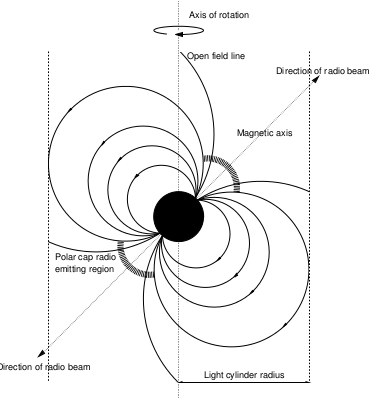
\includegraphics[width=0.9\textwidth]{figures/image2.png}
  \caption{Image 2.}
  \label{fig:gwb_search_2}
\end{figure}

Most known pulsar exhibits pulse periods \(P \sim 0.5\ \mathrm{s}\), which increase at rates \(\dot{P} \sim 10^{-15}\ \mathrm{s/s}\). The relationship is as follow, and is commonly analysed via the p pdot diagram

\begin{figure}[H]
  \centering
  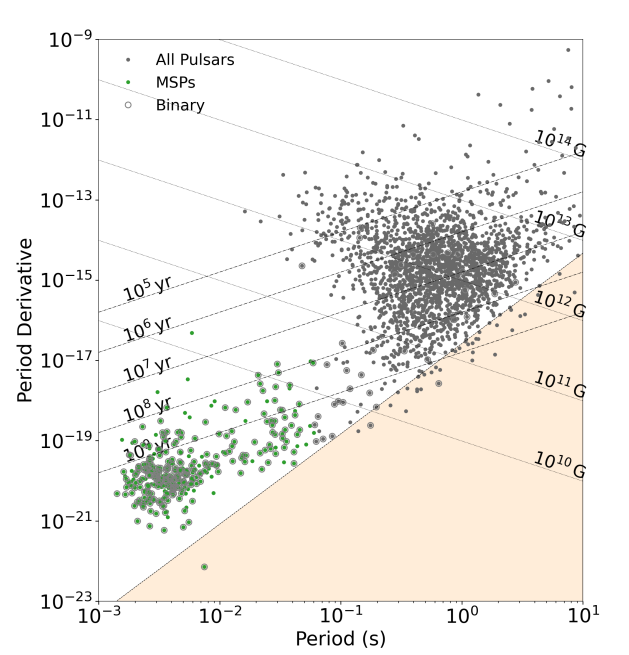
\includegraphics[width=0.8\textwidth]{figures/image29.png}
  \caption{Scatter plot of noise correlations.}
\end{figure}

(Manchester R. N., Hobbs G. B., Teoh A., Hobbs M., 2005)

Marked green in the figure are the population of millisecond pulsars, first discovered by (Alpar M. A., Cheng A. F., Ruderman M. A., Shaham J., 1982). Most of which exist in binary systems (marked by open grey circles). Typical companions are white dwarfs, main-sequence stars, or other neutron stars. A standard formation scenario of millisecond pulsars are of the following: the primary star explodes into a neutron star, often ejecting the system or imparting a "kick."  For those few binaries that remain bound, and in which the companion is sufficiently massive to evolve into a giant and overflow its Roche lobe, the old spun-down neutron star can 'spun-up' as a pulsar by accreting matter and angular momentum at the expense of the orbital angular momentum of the binary system.

\begin{figure}[H]
  \centering
  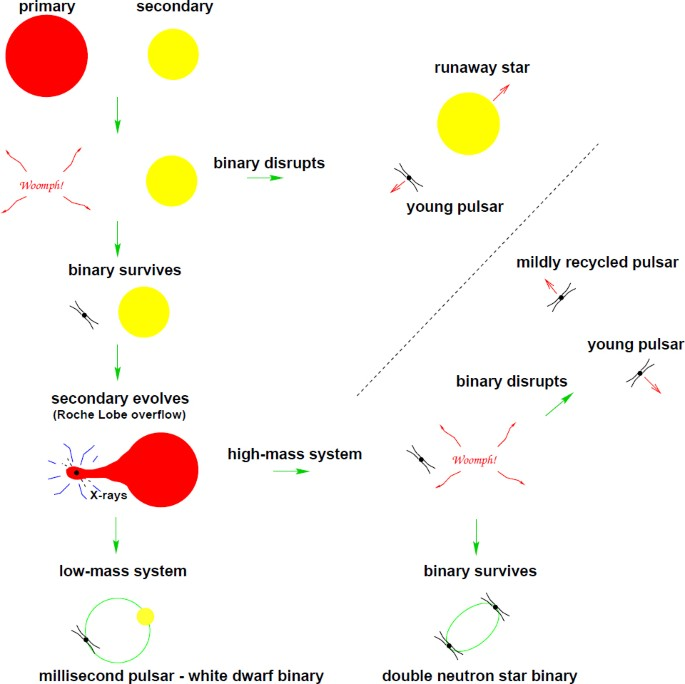
\includegraphics[width=0.7\textwidth]{figures/image1.jpg}
  \caption{Image 1.}
\end{figure}

(https://link.springer.com/article/10.12942/lrr-2008-8)

\subsection{Pulsar timing}

Pulsar timing is the precise measurement of pulse times of arrival (TOAs) in order to track every rotation of the neutron star. We obtain the observed pulse profile by averaging 8-second subintegrations over the full observation and 32 frequency channels. This profile is then cross-correlated with a high-SNR standard template to determine the pulse phase. The TOAs (initially referenced to an observatory clock) are then corrected for known delays and transformed into a common reference frame. For example, clock offsets are applied (e.g. UTC→TDB), and the TOAs are converted to barycentric dynamical time at the Solar-System barycentre. 

Propagation delays, such as dispersion in the interstellar medium, gravitational propagation effects, and tropospheric delays, alongside the pulsar's own motion (binary orbit, proper motion) are included in the timing model. In practice, one fits a deterministic timing model (including spin frequency, spin-down, position, DM, and orbital parameters if present) to the full set of TOAs. 

In practice, one  The observations are written in psrfits (Hotan, van Straten \& Manchester 2004) format, containing 256s((?)) subintegrations of the pulsar observation at a phase resolution of 1024 bins, with four polarization products, with the early data being recorded with 928 channels3 and the latter data with 1024 frequency channels.

A \emph{subintegration} is the averaging of folded pulse profiles over a short time interval (here typically 256 s) to produce a single profile per subintegration while preserving time resolution across the observation. Subintegrating reduces data volume and increases SNR for each profile used in template matching, but choices in subintegration length (for example \texttt{mode} vs \texttt{max}) trade time resolution against per-subintegration SNR and can change TOA uncertainties and error estimation. The \texttt{max} files adopt the largest allowable subintegration such that each subintegration meets an SNR threshold; inconsistent subintegration strategies hence affect downstream noise estimates and combining bands (UHF/L-band).

The timing residuals are defined as the differences between the observed TOAs and those predicted by the timing model. These residuals contain the imprints of any unmodeled effects or signals, including white and red noise processes, as well as low-frequency gravitational waves.

In the MeerKAT PTA analysis, TOAs are extracted using a 32-subband frequency resolution scheme, in which each observation is divided into 32 contiguous frequency channels before template matching and TOA estimation (Spiewak et al., 2023). This method preserves chromatic timing information, improves the modelling of dispersion measure variations, and enhances sensitivity to frequency-dependent effects such as scattering and pulse profile evolution.


\section{Noise models \& timing residuals}

Timing residuals include a variety of stochastic noise processes. These are conventionally split into white noise (high-frequency, uncorrelated) and red noise (low-frequency, correlated) components. White noise arises from random processes including instrumental uncertainties and pulse-phase jitter, and is often parametrized phenomenologically by three parameters: EFAC (a multiplication factor on TOA uncertainties), EQUAD (an added white-noise variance, added in quadrature), and ECORR (an epoch-correlated "jitter" term). Red noise consists of timing noise that can mimic the long-timescale signals of interest. It includes achromatic components (frequency-independent), such as intrinsic "spin noise" or irregularities in the pulsar's rotation, and chromatic components (frequency-dependent). In practice, one commonly models one achromatic red process (a power-law spin/noise term) plus chromatic processes for DM variations, scattering delays, solar wind fluctuations, etc.. These noise models are fitted to the timing residuals to isolate deterministic trends, mainly the GWB, from stochastic fluctuations that could smear the signal.

The methods used to determine these noise processes can all be classified as Monte Carlo Markov Chains (MCMC), two different packagews with slightly different functionalities will be later introduced and used in projects 2 and 3, namely \texttt{tempered\_nest} and \texttt{ptmcmc}.

\section{GWB \& PTA}

First proposed by Albert Einstein in his infamous general theory of relativity (Einstein, A. (1915) Die Feldgleichungen der Gravitation. Sitzungsberichte der Königlich Preu\ss ischen Akademie der Wissenschaften, 48, 844-847), gravitational waves had been indirectly detected by Hulse, Taylor, and collaborators by observing binary pulsars in 1976. A century after its proposal, the LIGO experiment provided the first direct detection of gravitational waves. 

The MPTA collaboration have detected ? sigma significance GWB in Data Release 2

\newpage

\section{Project 1: Cuts on unfiltered data and comparison to the `first pass' dataset}

\subsection{Methods}

\subsubsection{Obtaining the data}
The unfiltered data was obtained in the form of .par(parameter) and .tim(timing) files.

The .par files were obtained directly from: \texttt{/fred/oz002/users/mmiles/MPTA\_GW/partim\_frank/pp\_8}

The .tim files were obtained by concatenating all observation .tim files into a single .tim file for a pulsar: \texttt{/fred/oz005/timing\_processed/\{psrname\}/2*/?/timing/PTA/J*\_chopped.32ch\_1p\_mode*ar.tim}

As seen in the naming convention, the tim files chosen will possess the following properties:
\begin{itemize}
  \item 32 sub-channels (explained in intro)
  \item 1 total polarisation product -- only the total intensity kept, polarisation information is discarded
  \item `mode' refers to subintegrating once over one usual observation period (256s).
    \begin{itemize}
      \item Sometimes these files were empty, `max' files were used instead, which means the observation was subintegrated the maximum amount of time for the SNR of each subintegration to be higher than a certain(?) value.
    \end{itemize}
\end{itemize}

\subsubsection{Cleaning the data}
The method for cleaning the data imitated the procedure in the ASTRAL report, with slight modifications in the code used and in the specific cutoff thresholds applied.

All cuts were applied at the subband level, meaning that individual sub-channels failing the filtering criteria could be removed without discarding the entire observation. However, this creates the issue that some observations retain only a small number of subbands. In such cases, a single subband may disproportionately represent the entire observation, introducing artifacts such as systematic offsets and complications in modeling chromatic effects. To mitigate this, all observations with fewer than five surviving subbands were removed.

The signal-to-noise ratio (SNR) cutoff was set at 10. All observations with TOA uncertainties greater than 10 microseconds were discarded.

The minimum observation length was set to 128 seconds, and long observations made with the UHF band were removed because they are difficult to combine consistently with L-band observations due to differing frequency coverage and noise characteristics. (This issue was later addressed by others to make use of the UHF band data, but was not included in this analysis)

Further, all observations with reduced chi-squared values (per subband) greater than 3.6 were excluded, based on the analysis performed in the ASTRAL report.

For some pulsars, the problem arose that most of their observations failed a particular criterion (e.g., large TOA uncertainty), leaving very little usable data after cleaning. To address this, a safeguard was implemented: if a single criterion rejected more than 30\% of a pulsar's data, that criterion was relaxed, and the cutoff for that pulsar was determined manually (see appendix for specific cutoffs).

Two pulsars, J1843-1448 and J0900-3144, were removed from the dataset entirely, as consistent removal criteria could not be determined for them.


\subsection{Results and analysis}
In this project and project 3, the optimal statistic package was used to estimate the significance of gravitational waves in the data. It is a fast, frequentist estimator that computes a weighted sum of cross-correlations between pulsar timing residuals to estimate the amplitude and SNR of spatial correlation templates (e.g. the Hellings--Downs quadrupole or a dipole). It is useful for quick scans and for comparing template SNRs across many data cuts. 

As shown in Figure~\ref{fig:gwb_search_2}, it is straightforward to overplot a dipolar correlation on the same axes as the quadrupolar Hellings--Downs curve, and by eye the two can be difficult to distinguish---raising the concern that an apparent HD signal could instead be a dipolar signature arising from ephemeris errors.

Quantitatively, although the optimal-statistic returns a high signal-to-noise ratio (SNR) for the HD template, it also yields a comparably high SNR for the dipole template. This suggests that the putative HD detection may be contaminated by solar-system ephemeris errors or other systematics that mimic a dipolar pattern.

To investigate further, I applied a set of data cuts based on several criteria: Sun--pulsar separation (removing observations below various elevation angles), dispersion measure thresholds, exclusion of all data from 2019 and 2025, and manual excision of outliers. The strongest HD SNR overall (15.52) came from the DM\(\leq\)60 pc\,cm\(^{-3}\) cut. However, when simultaneously excluding both 2019 and 2025 data, the HD SNR remains healthy (8.75) while the dipole SNR falls to only 3.83---yielding the largest disparity between quadrupole and dipole significance.

This outcome is plausible: early MeerKAT observations in 2019 were affected by non-optimal hardware and software settings, and post-2024 timing may suffer from unmodeled solar-wind or ephemeris changes (since our noise model was calibrated on data through mid-2024). Removing both epochs thus minimizes dipolar systematics while preserving a robust HD correlation.

\begin{table}[H]
\centering
\begin{tabular}{lcc}
\toprule
Directory & SNR\_HD & SNR\_dipolar \\
\midrule
GWB\_search\_2 & 12.237026420376978 & 10.582305696757597 \\
GWB\_search\_2\_angle10 & 12.036049434027658 & 10.791268727744255 \\
GWB\_search\_2\_angle20 & 11.457201595506715 & 10.82832353432228 \\
GWB\_search\_2\_angle30 & 11.554110414653067 & 10.879401568394524 \\
GWB\_search\_2\_angle50 & 7.631584657002278 & 8.27166492385602 \\
GWB\_search\_2\_dm100 & 14.276981264457598 & 13.43022838088923 \\
GWB\_search\_2\_dm20 & 0.6281049361049306 & 2.0616303541216223 \\
GWB\_search\_2\_dm40 & 11.46340934603799 & 6.658734626707023 \\
GWB\_search\_2\_dm60 & 15.523151321473124 & 13.6080501815082 \\
GWB\_search\_2\_dm80 & 15.388922036086159 & 13.891987552255918 \\
GWB\_search\_2\_no2019 & 15.144103974568402 & 11.902882940519328 \\
GWB\_search\_2\_no2025 & 6.952835904140578 & 4.935448839925726 \\
GWB\_search\_2\_no2025\_2019 & 8.74795707430896 & 3.8307057216285947 \\
GWB\_search\_2\_psrcut & 14.111231021468354 & 10.587572649245462 \\
GWB\_search\_2\_psrcut2 & 13.636544993177322 & 10.288101047436156 \\
GWB\_search\_2\_psrcut2\_no\_pattern & 11.066674346944119 & 9.502086467225705 \\
GWB\_search\_2\_psrcut2\_pattern & 14.703701066347413 & 11.360942952496437 \\
\bottomrule
\end{tabular}
\caption{Summary of optimal-statistic SNRs across different data cuts.}
\end{table}

\begin{figure}[H]
  \centering
  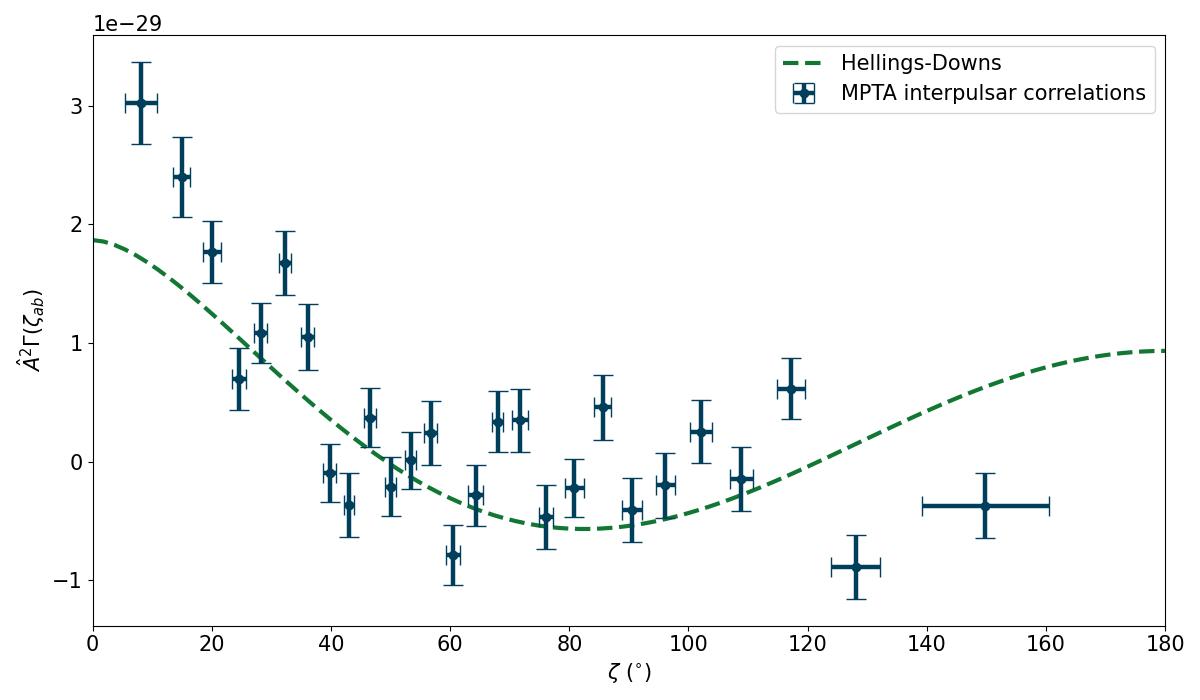
\includegraphics[width=0.75\textwidth]{figures/image9.png}
  \caption{Residuals after cleaning (Project 1).}
\end{figure}


\newpage

\section{Project 2: Noise analysis with Hendrik's FD removed files}


\subsection{Method}
\emph{pBilby} (parallel Bilby) is the parallelised interface to the Bilby Bayesian-inference framework. It is well-suited to evidence-based model comparison on individual pulsars because it can compute marginal likelihoods (evidences) efficiently in high-dimensional spaces and supports samplers that handle multimodal posteriors. In this work pBilby was used to compare evidence for white and red noise components between FD-removed and \texttt{third\_pass} templates, which helps identify where template changes systematically alter parameter constraints or evidence ratios.

In this analysis, I used pbilby to compare the evidence levels of various noise parameters for the same pulsar but created from different template, namely the FD-removed dataset created by Hendrik and the original third\_pass dataset.

The pulsars are generally classified as "well behaved", taken from a list given by Hendrik, or "poorly behaving". The criteria used to determine this is the plots of DM\_observed vs DM\_predicted (using the Taylor series in the .par file). By removing the FD parameters, the new template should recover a DM\_predicted aligning closer with DM\_observed by removing Freuquency dependent parameter which absorb some of the DM noise. Poorly behaving pulsars generally have a large offset DM\_observed and DM\_predicted, and/or having a DM\_predictred taylor polynomial which doesn't mimic the pattern of DM\_observed well.

Here, J1125-5825 is provided as an example as a poorly behaving pulsar, though the pattern  resembles decently, there is a large offset of $\sim 0.3$ DM units remaining even after the FD removal.

\begin{table}[H]
  \centering
  \begin{tabular}{|c|c|}
    \hline
    \begin{minipage}{0.48\textwidth}
      \centering
      \begin{subfigure}[b]{\linewidth}
        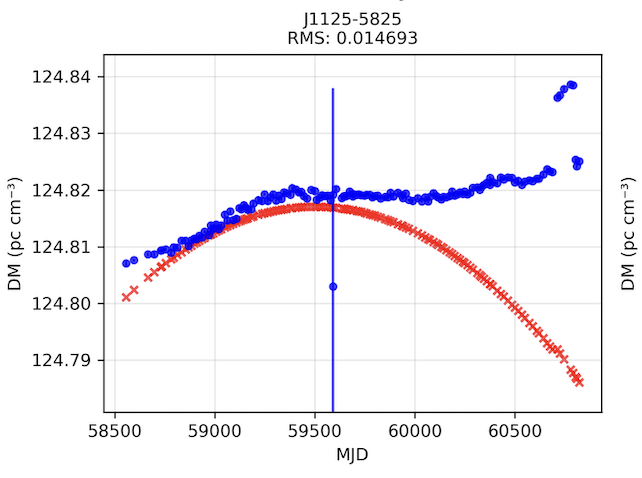
\includegraphics[width=\linewidth,height=0.35\textheight,keepaspectratio]{figures/image19.png}
        \caption{FD\_removed --- J1125-5825 (DM)}
        \label{fig:img19}
      \end{subfigure}
    \end{minipage}
    &
    \begin{minipage}{0.48\textwidth}
      \centering
      \begin{subfigure}[b]{\linewidth}
        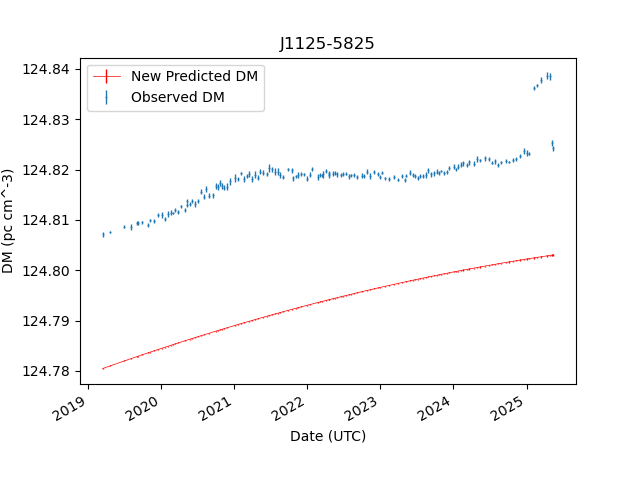
\includegraphics[width=\linewidth,height=0.35\textheight,keepaspectratio]{figures/image13.png}
        \caption{third\_pass --- residuals comparison}
        \label{fig:img10}
      \end{subfigure}
    \end{minipage}
    \\
    \hline
  \end{tabular}
  \caption{Comparison of FD\_removed and third\_pass results.}
  \label{tab:twopanel}
\end{table}


The first test case is a "well-behaving" pulsar J1911-1114

Evident in the plot below, notice the offset is around 0.002 DM units

\begin{figure}[H]
  \centering
  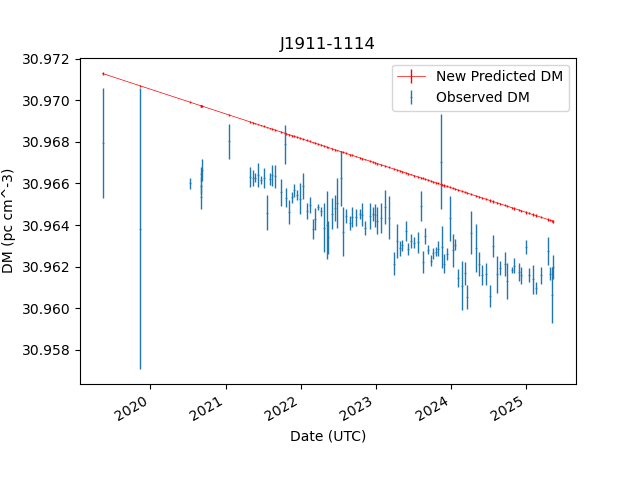
\includegraphics[width=0.8\textwidth]{figures/image10.png}
  \caption{Evidence plot: FD-removed vs third\_pass.}
\end{figure}

% 1*3 table
\setlength{\tabcolsep}{10pt}    
\renewcommand{\arraystretch}{1.10}


\captionsetup[subfigure]{labelformat=simple}
\renewcommand\thesubfigure{(\alph{subfigure})}


When modelling the FD-removed data, significantly more parameters are well-constrained compared to the third\_pass data. This is reasonable, as only the DM terms are active in the .par file for the FD-removed data, leading to residual trends being absorbed into the noise model.

To enable a fairer comparison, we re-fit all timing model parameters in the .par file for the test pulsars. In the case of J1911-1114, most of the peaks in the corner plots appear similar between the two datasets. However, the FD-removed data shows a prominent peak for the TNEQuad parameter, suggesting systematic effects introduced by the new template. This was later determined to be likely caused by an underestimation of TOA uncertainties in the new template.

(For a better full picture, I decided to use the everything model (red + DM + CHROM + SW) instead of the predetermined choice for analysing the pulsars)

\subsubsection{Well beavhing pulsars}


\setlength{\tabcolsep}{10pt}  
\renewcommand{\arraystretch}{1.15}

\begin{figure}[H]
  \centering
  % Row 1
  \begin{subfigure}[b]{0.48\textwidth}
    \centering
    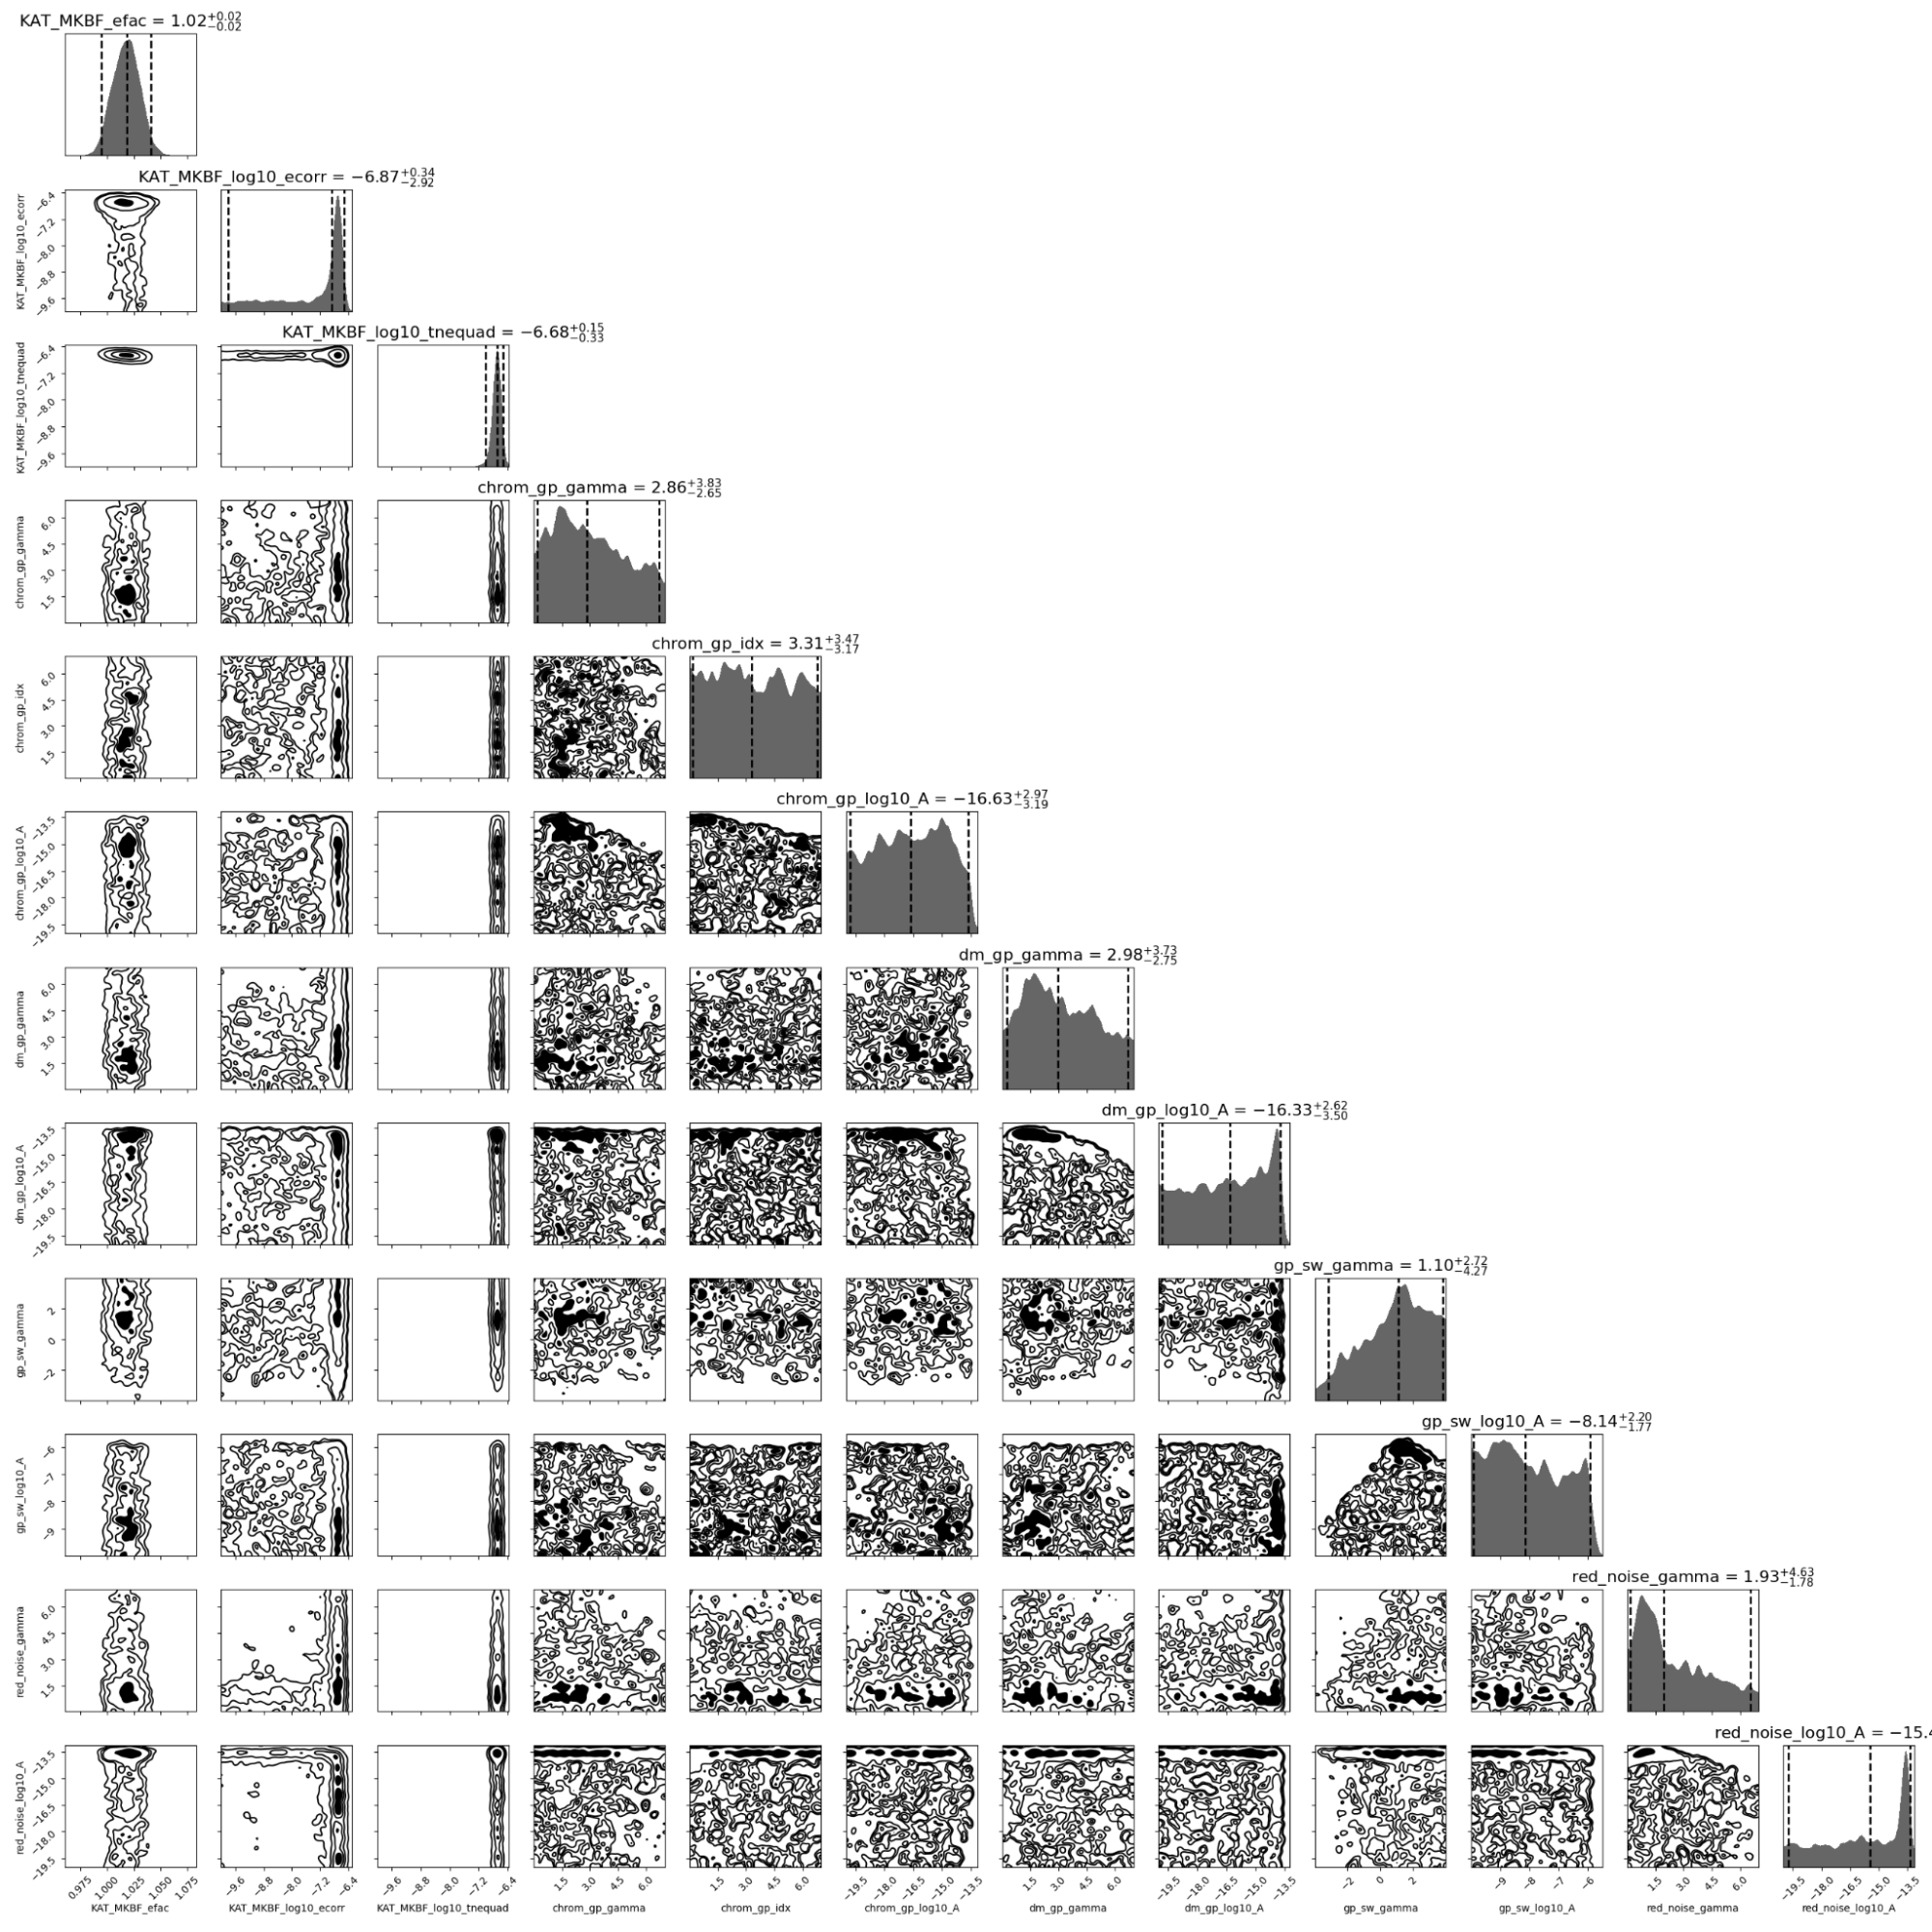
\includegraphics[width=\linewidth,height=0.33\textheight,keepaspectratio]{figures/image32.png}
    \caption{J0711-6830 (FD\_removed)}
    \label{fig:img1}
  \end{subfigure}
  \hfill
  \begin{subfigure}[b]{0.48\textwidth}
    \centering
    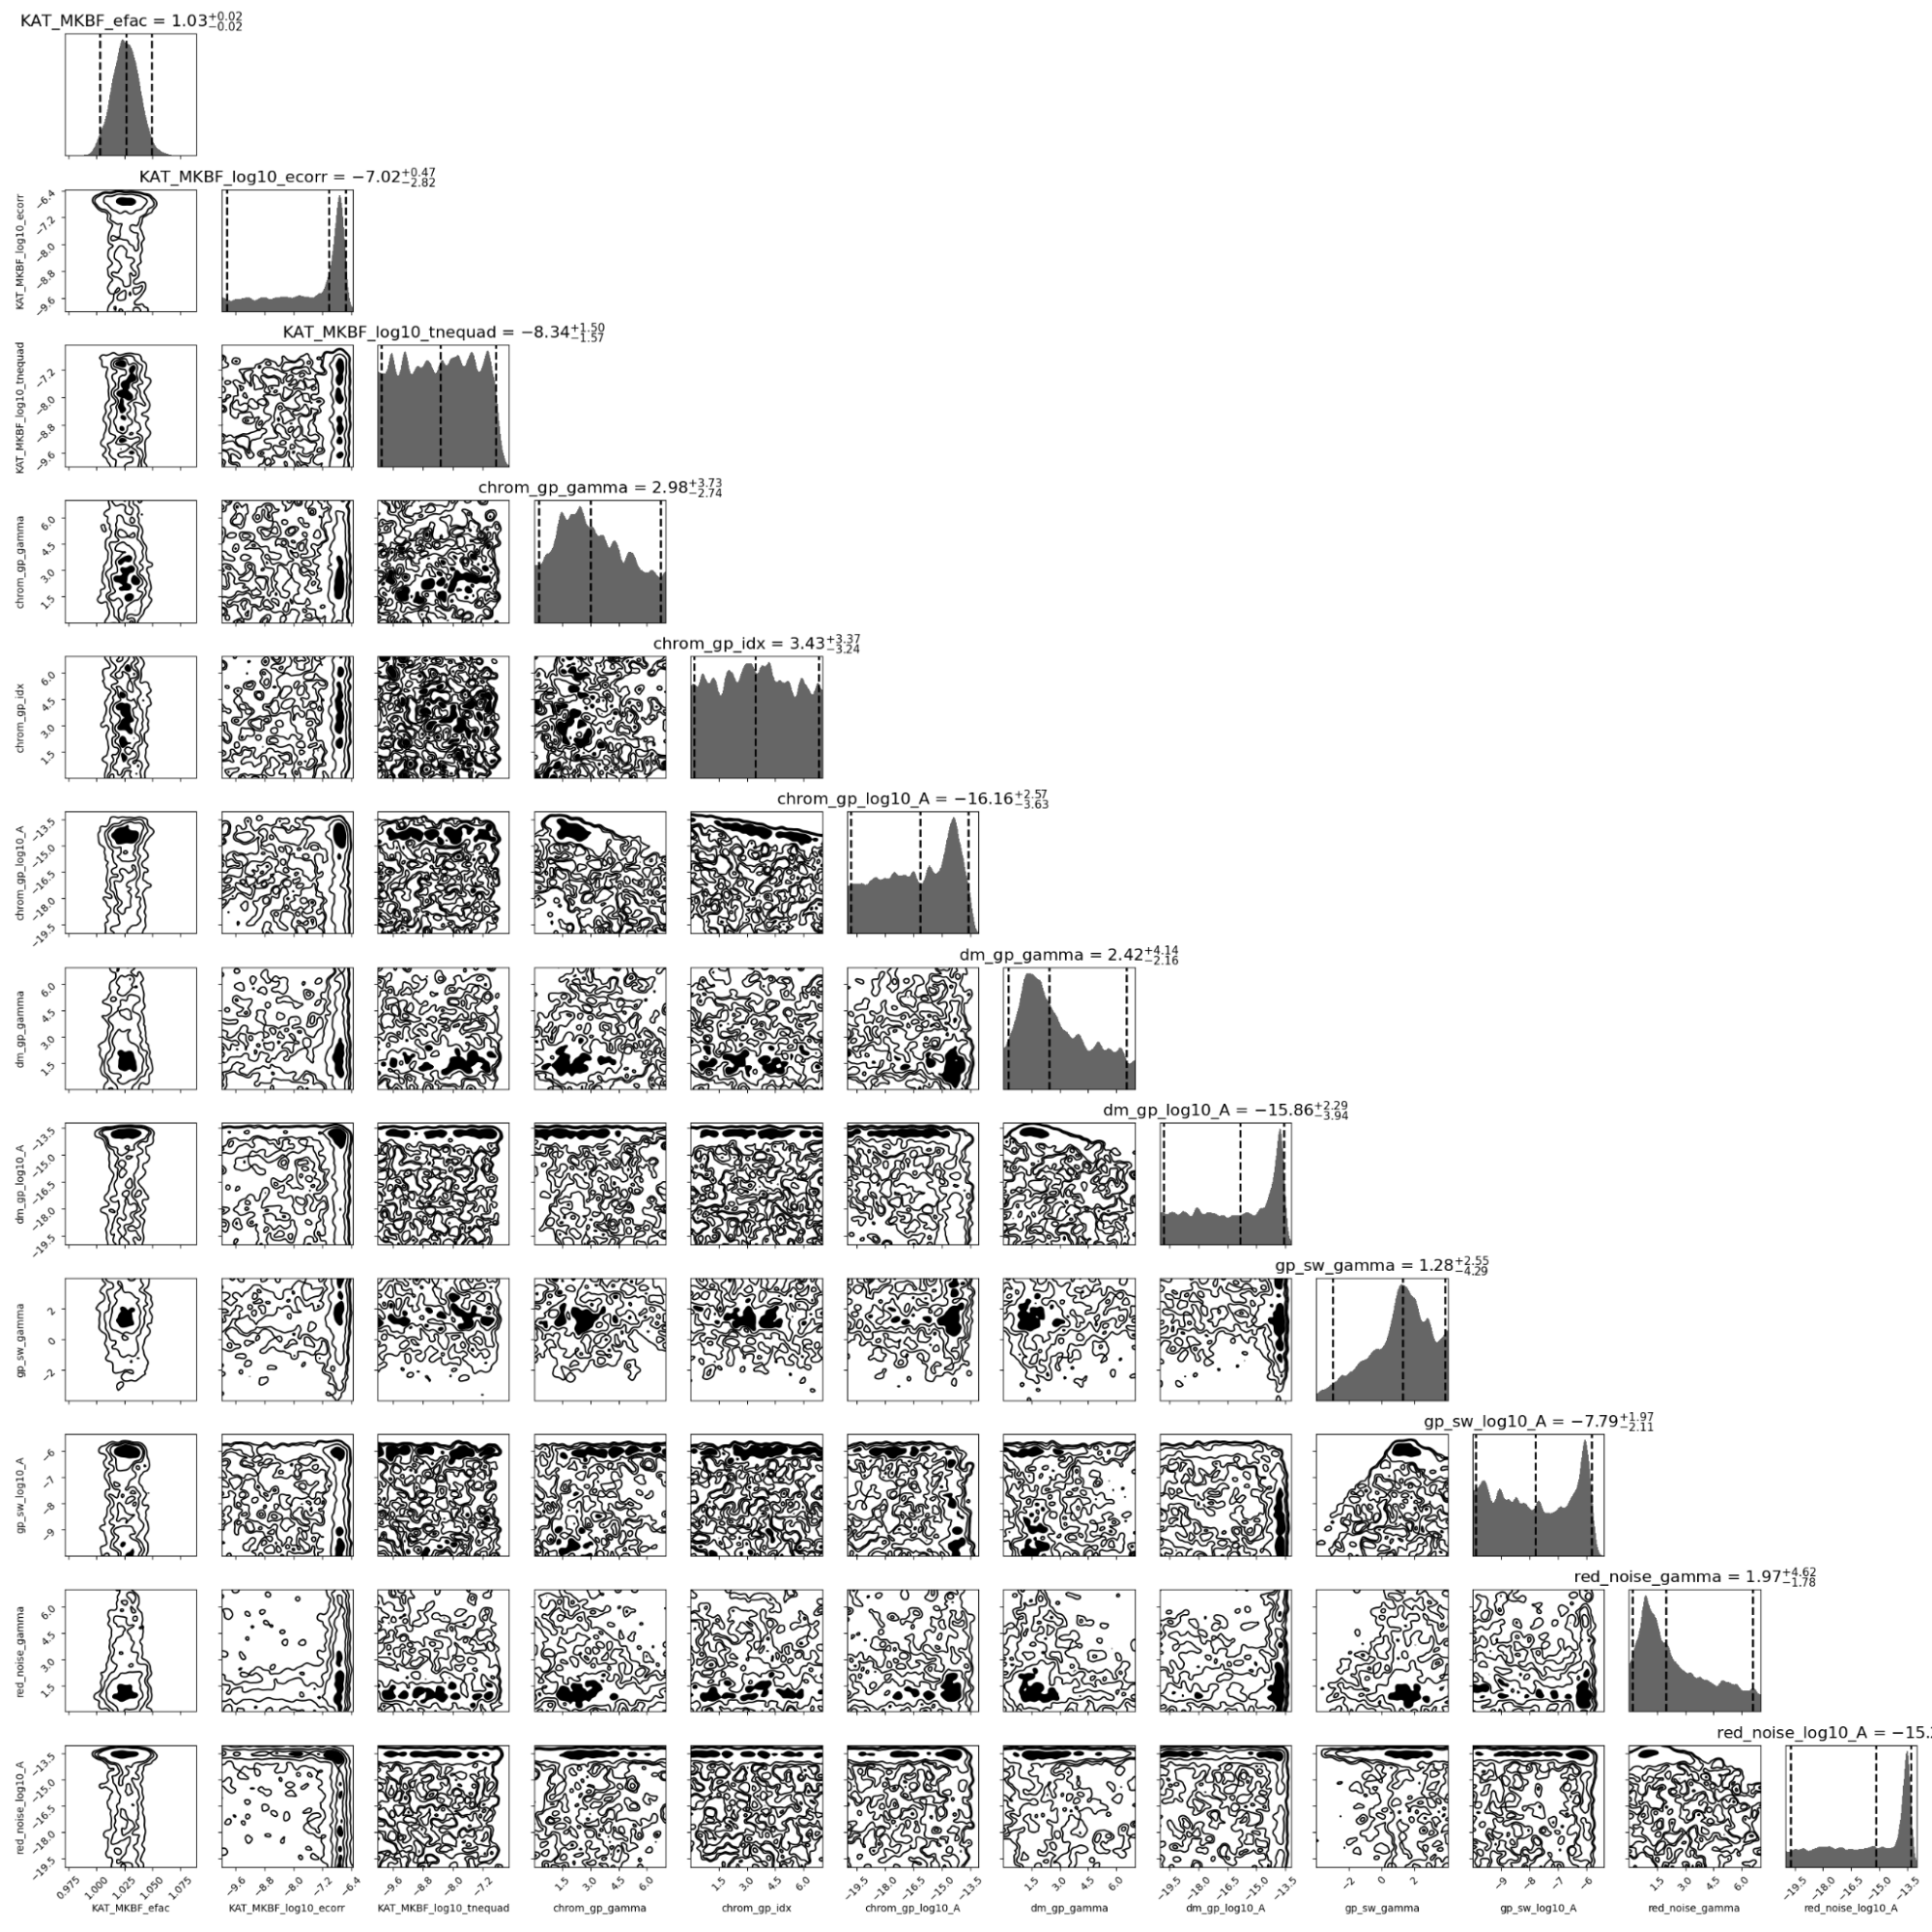
\includegraphics[width=\linewidth,height=0.33\textheight,keepaspectratio]{figures/image11.png}
    \caption{J0711-6830 (third\_pass)}
    \label{fig:img2}
  \end{subfigure}

  \vspace{10pt}

  % Row 2
  \begin{subfigure}[b]{0.48\textwidth}
    \centering
    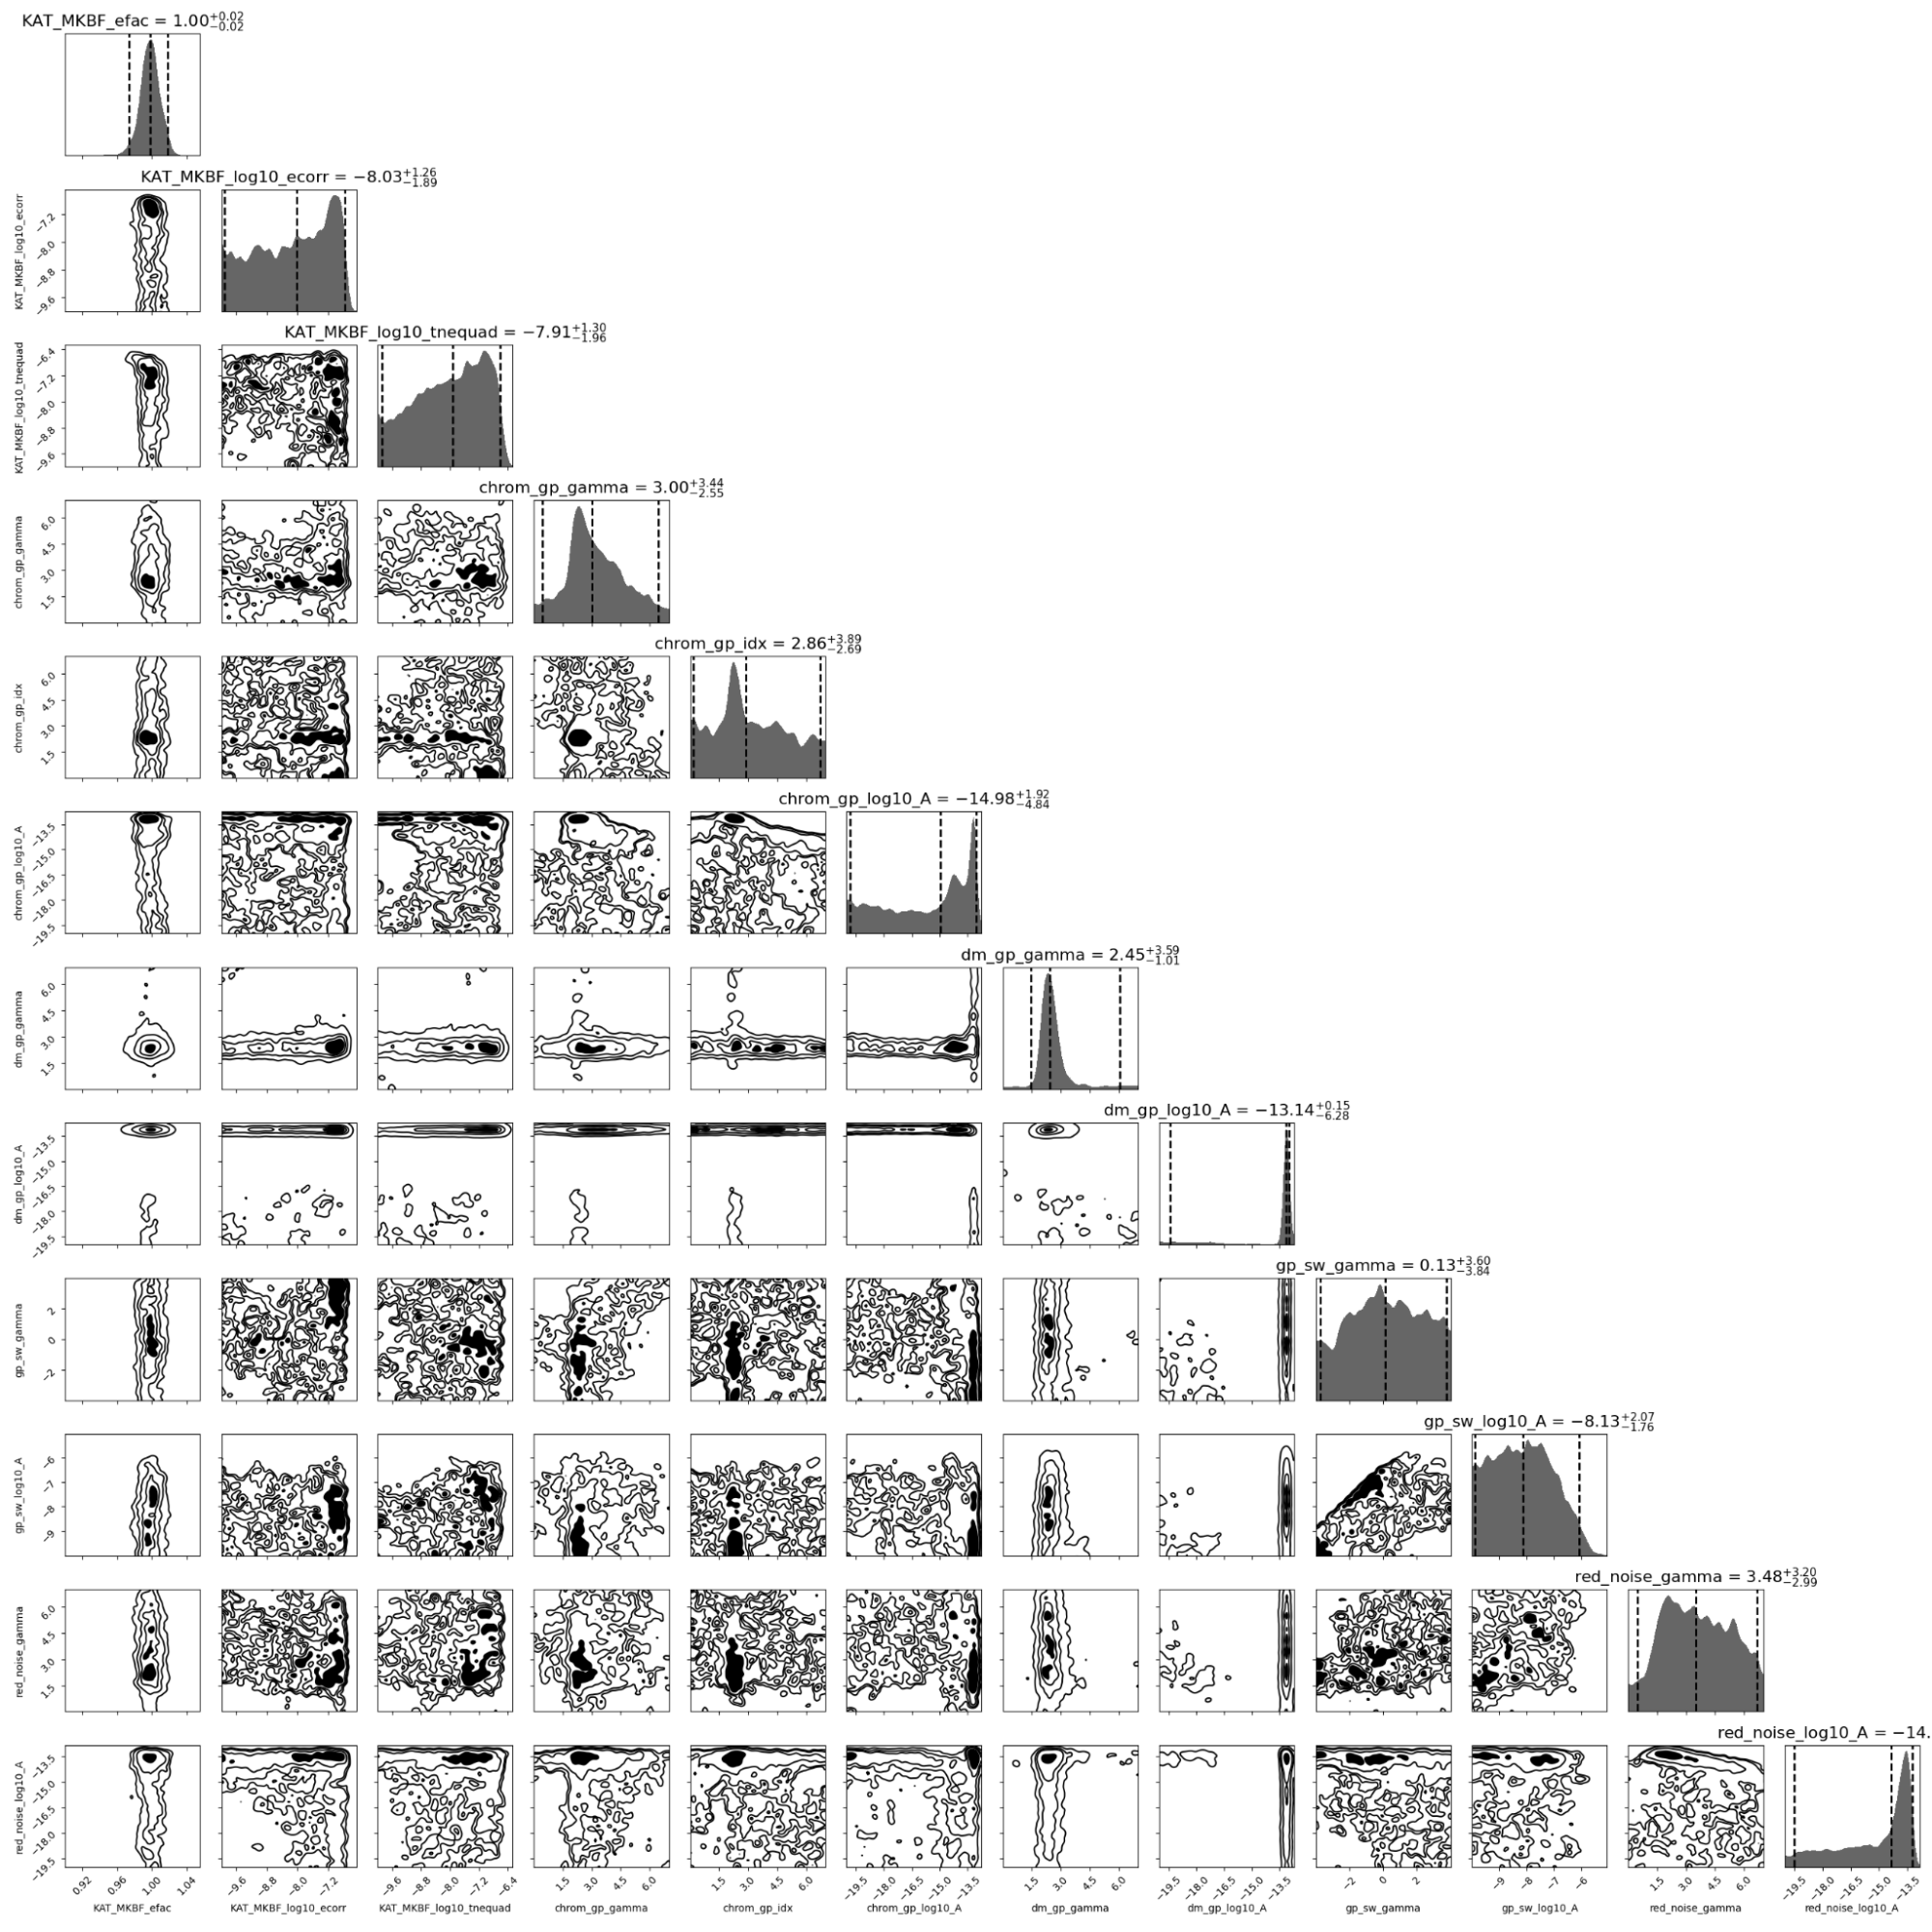
\includegraphics[width=\linewidth,height=0.33\textheight,keepaspectratio]{figures/image33.png}
    \caption{J1216-6410 (FD\_removed)}
    \label{fig:img3}
  \end{subfigure}
  \hfill
  \begin{subfigure}[b]{0.48\textwidth}
    \centering
    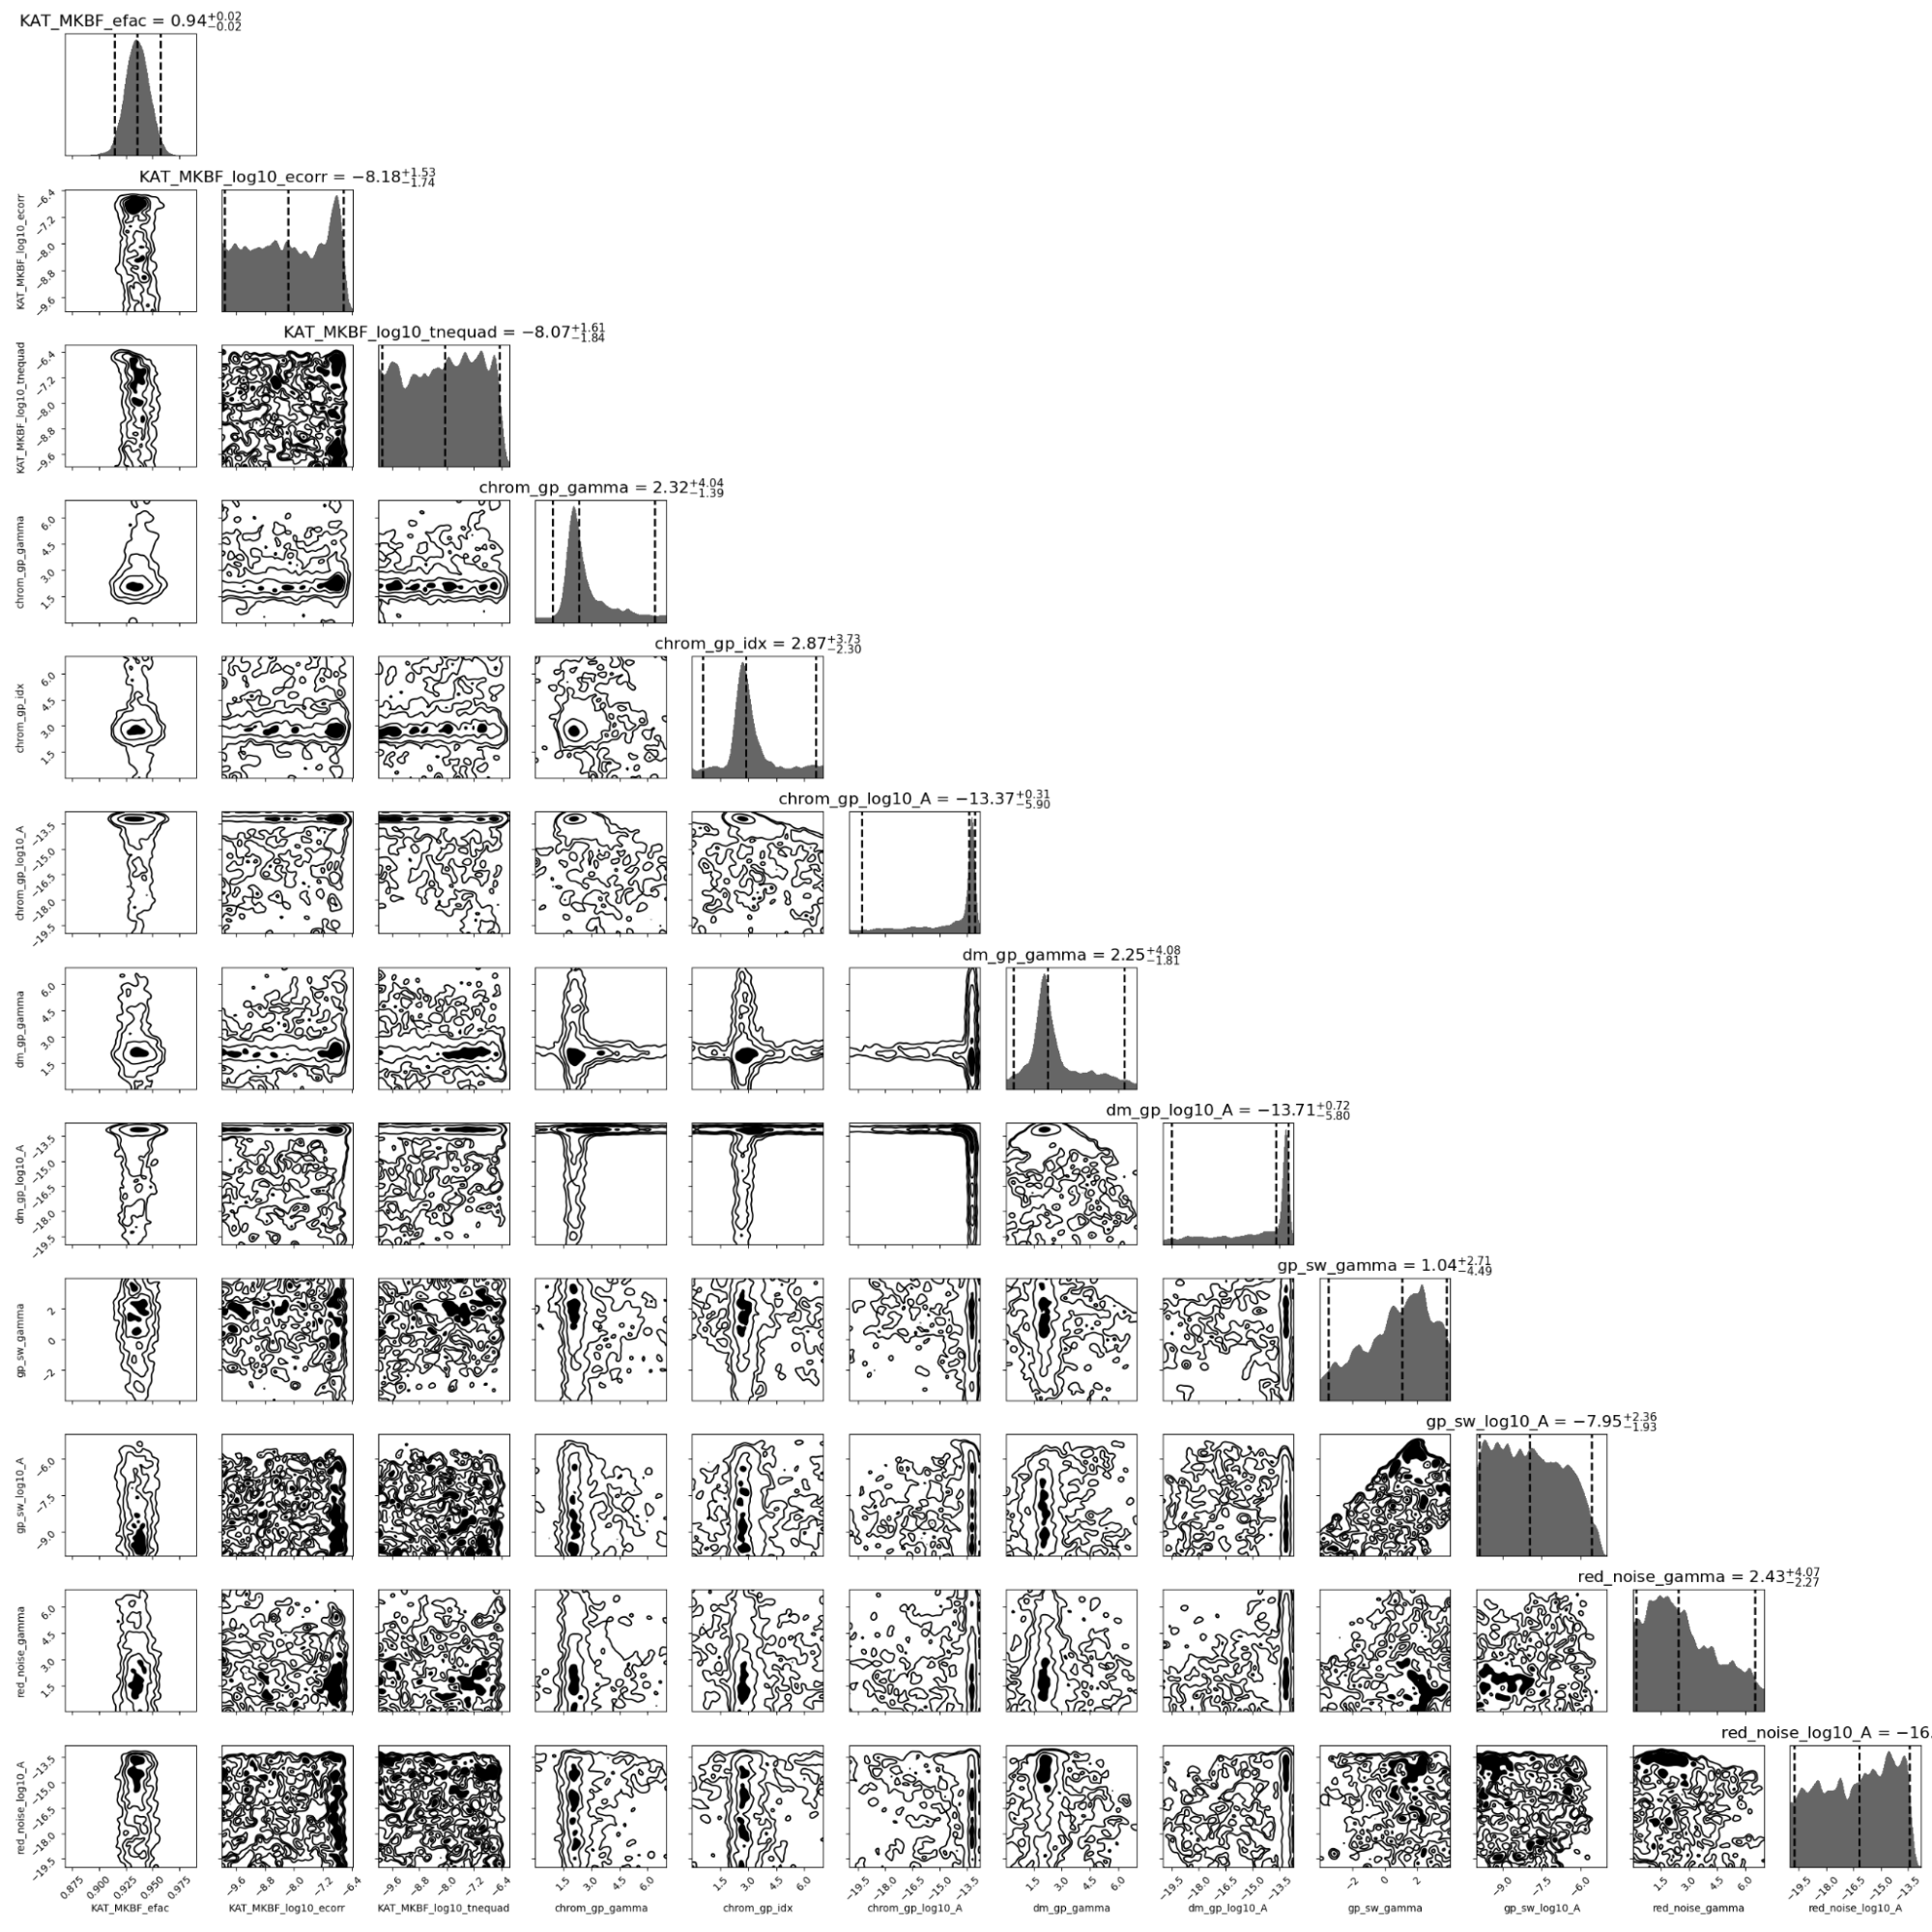
\includegraphics[width=\linewidth,height=0.33\textheight,keepaspectratio]{figures/image14.png}
    \caption{J1216-6410 (third\_pass)}
    \label{fig:img4}
  \end{subfigure}

  \vspace{10pt} 

  % Row 3
  \begin{subfigure}[b]{0.48\textwidth}
    \centering
    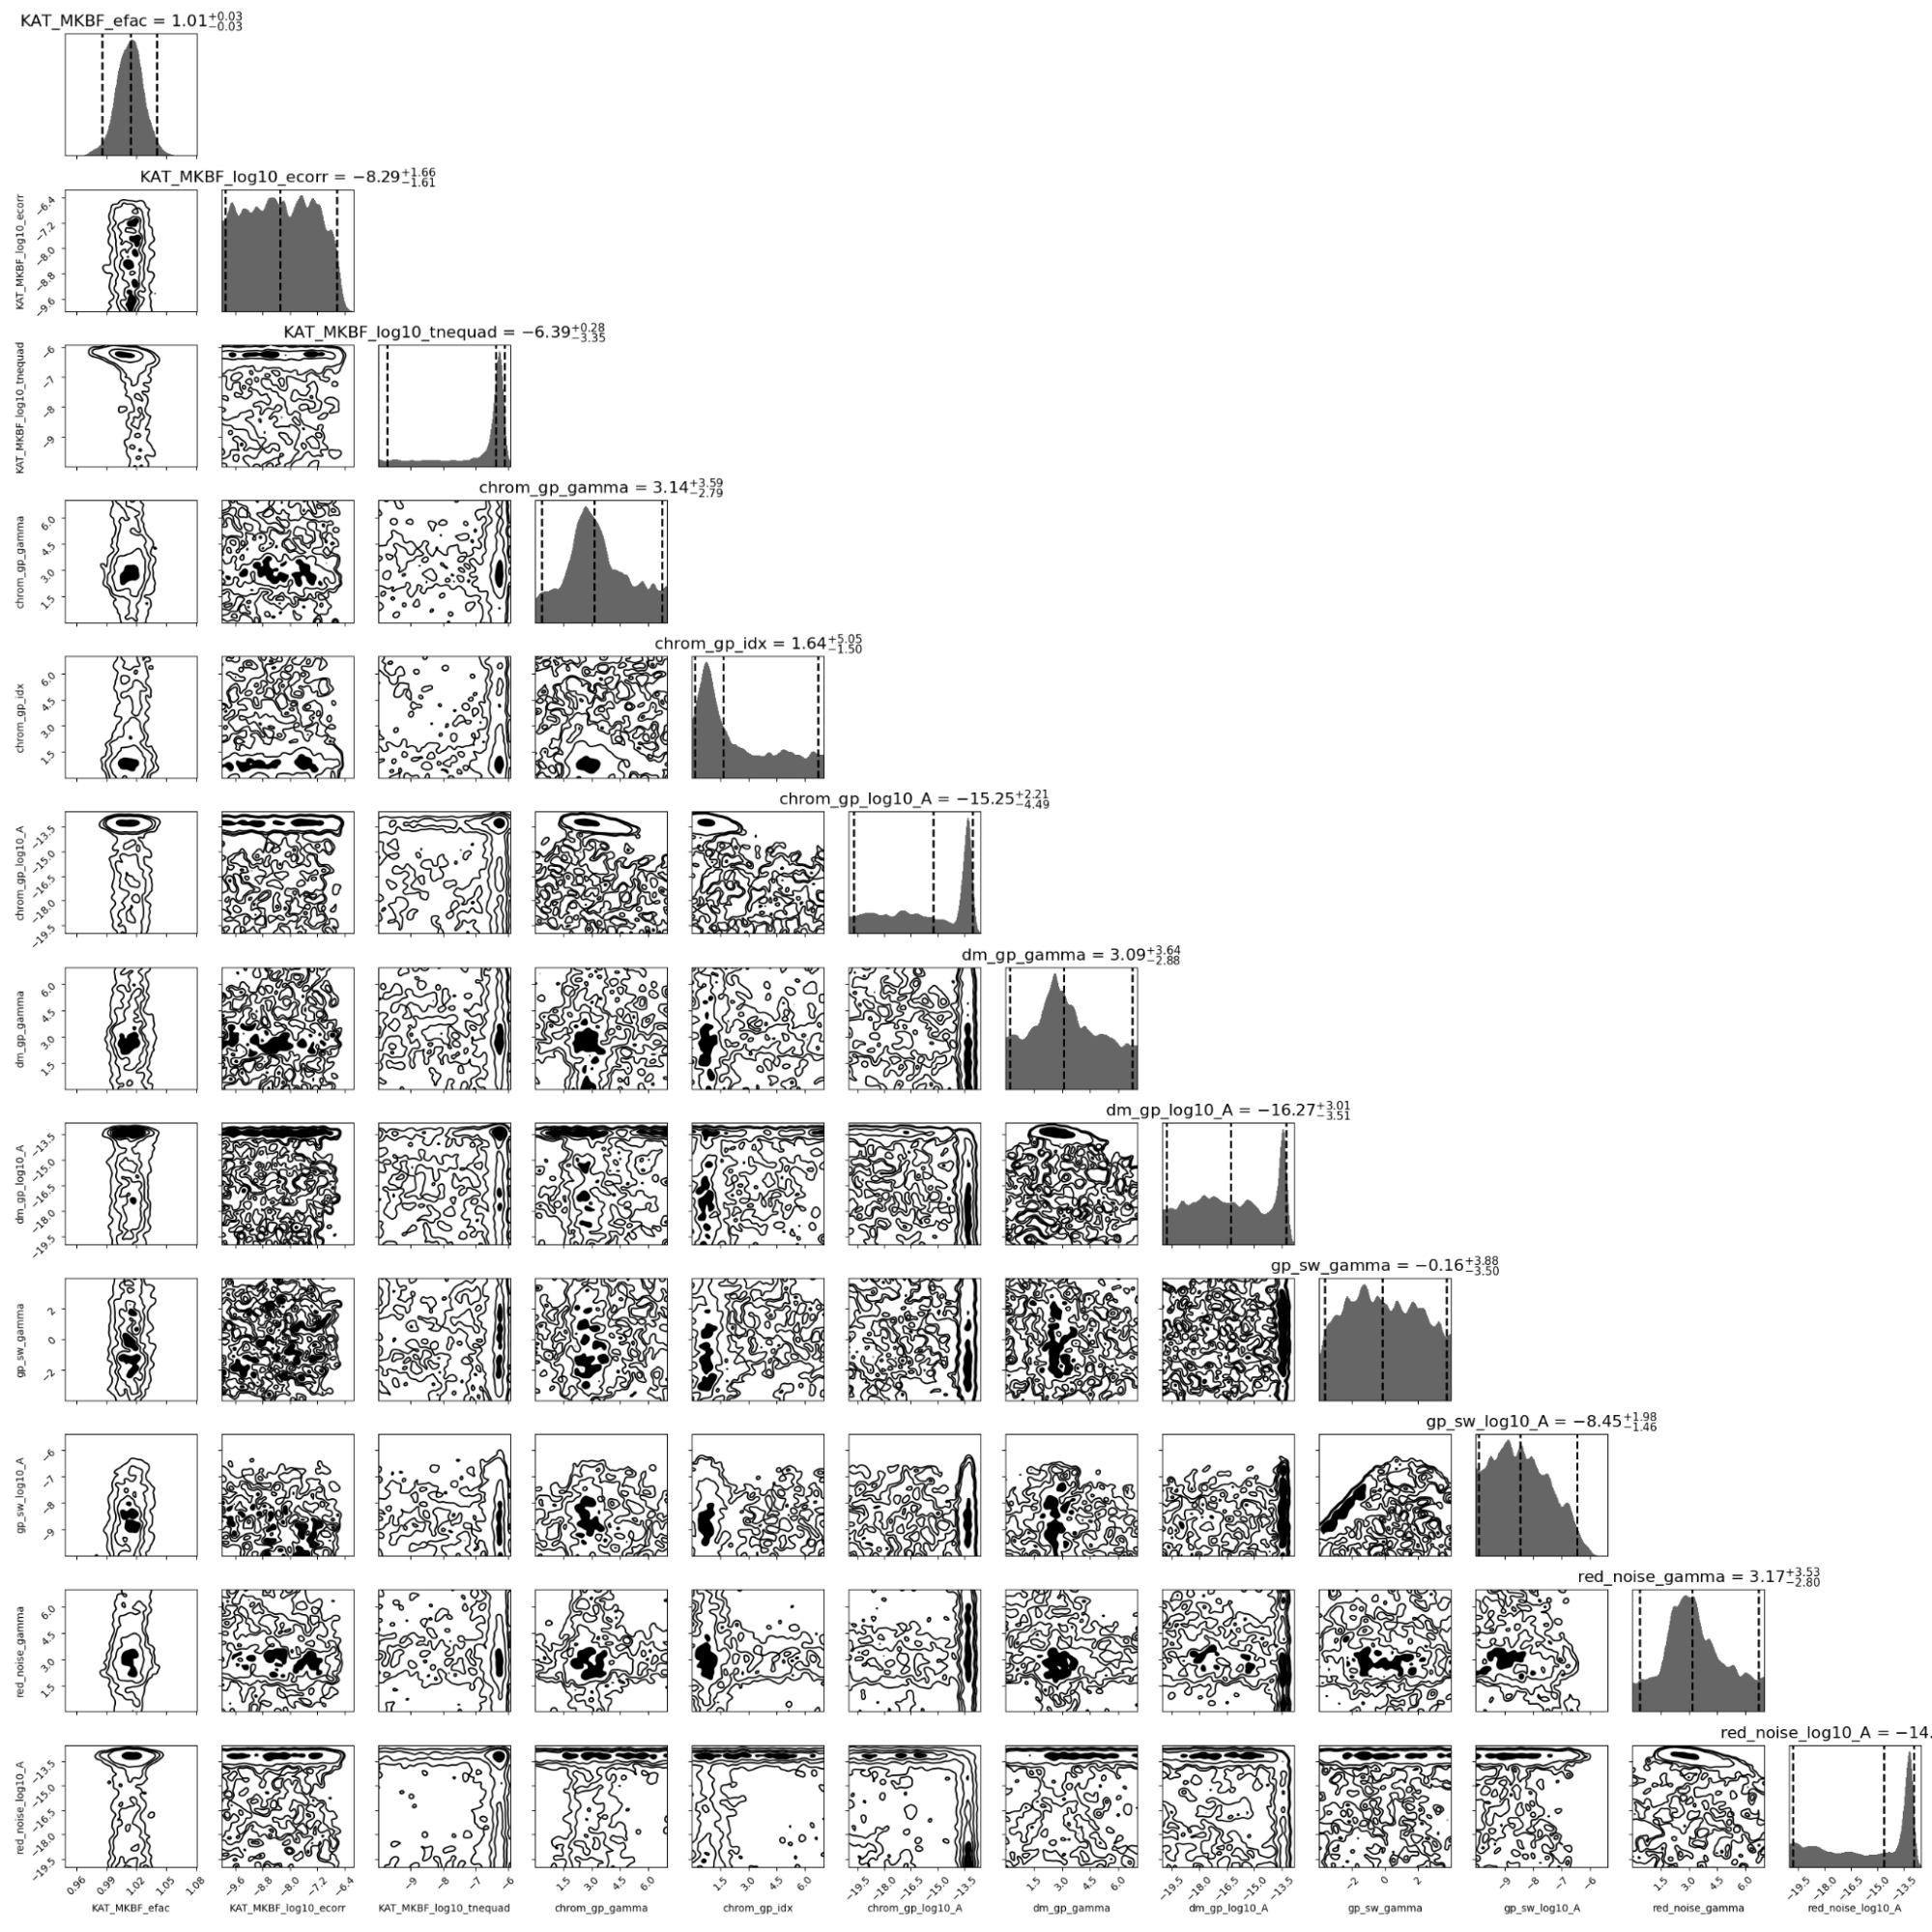
\includegraphics[width=\linewidth,height=0.33\textheight,keepaspectratio]{figures/image16.png}
    \caption{J1719-1438 (FD\_removed)}
    \label{fig:img5}
  \end{subfigure}
  \hfill
  \begin{subfigure}[b]{0.48\textwidth}
    \centering
    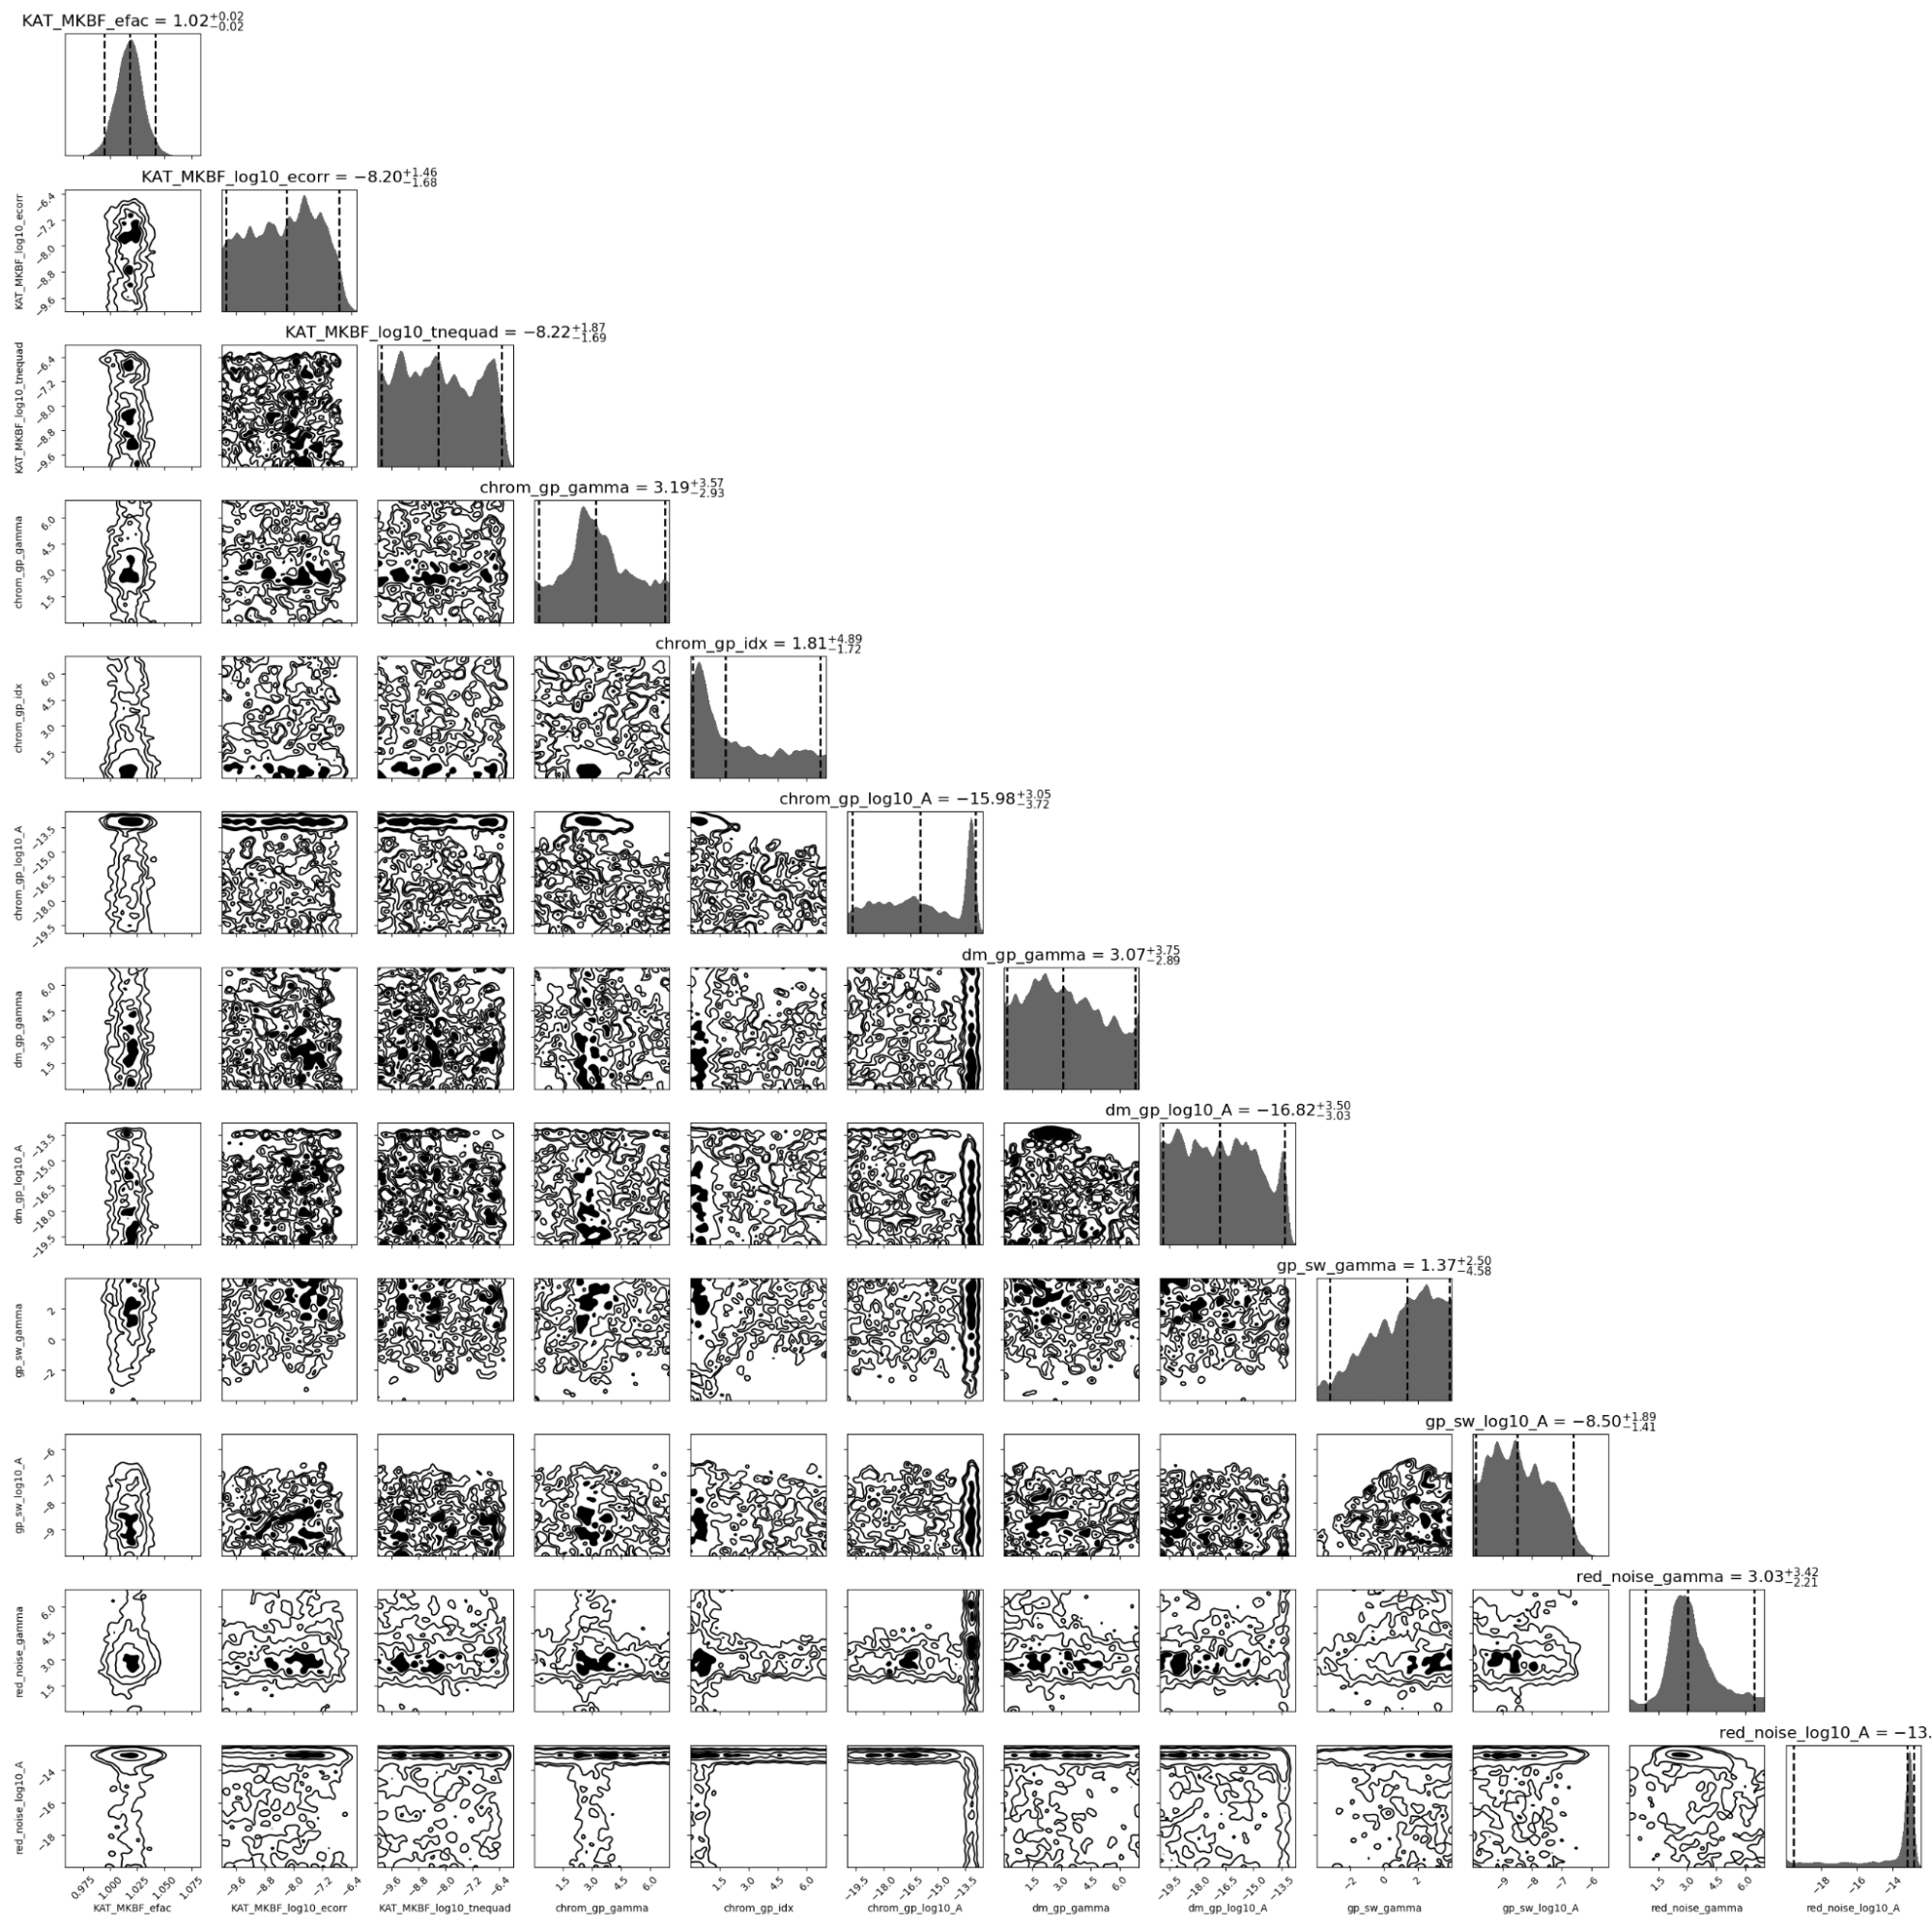
\includegraphics[width=\linewidth,height=0.33\textheight,keepaspectratio]{figures/image21.png}
    \caption{J1719-1438 (third\_pass)}
    \label{fig:img6}
  \end{subfigure}

  \caption{Global caption describing the 3×2 panel.}
  \label{fig:3x2_noborder}
\end{figure}




By eye, there is not much of a difference in all the noise parameter evidence except for equad, similar to J1911-1450 (expect for J1216-6410, for this there seems to be some evidence, but not that clear). As above, the reason predicted for this is from underestimation of error bars in the new templates.

\subsubsection{Poorly behaving pulsars}


\setlength{\tabcolsep}{12pt}  
\renewcommand{\arraystretch}{1.05} 


\captionsetup[subfigure]{labelformat=simple}
\renewcommand\thesubfigure{(\alph{subfigure})}

\begin{figure}[H]
  \centering
  \begin{tabular}{cc}
    % Top-left
    \begin{subfigure}[b]{0.48\textwidth}
      \centering
      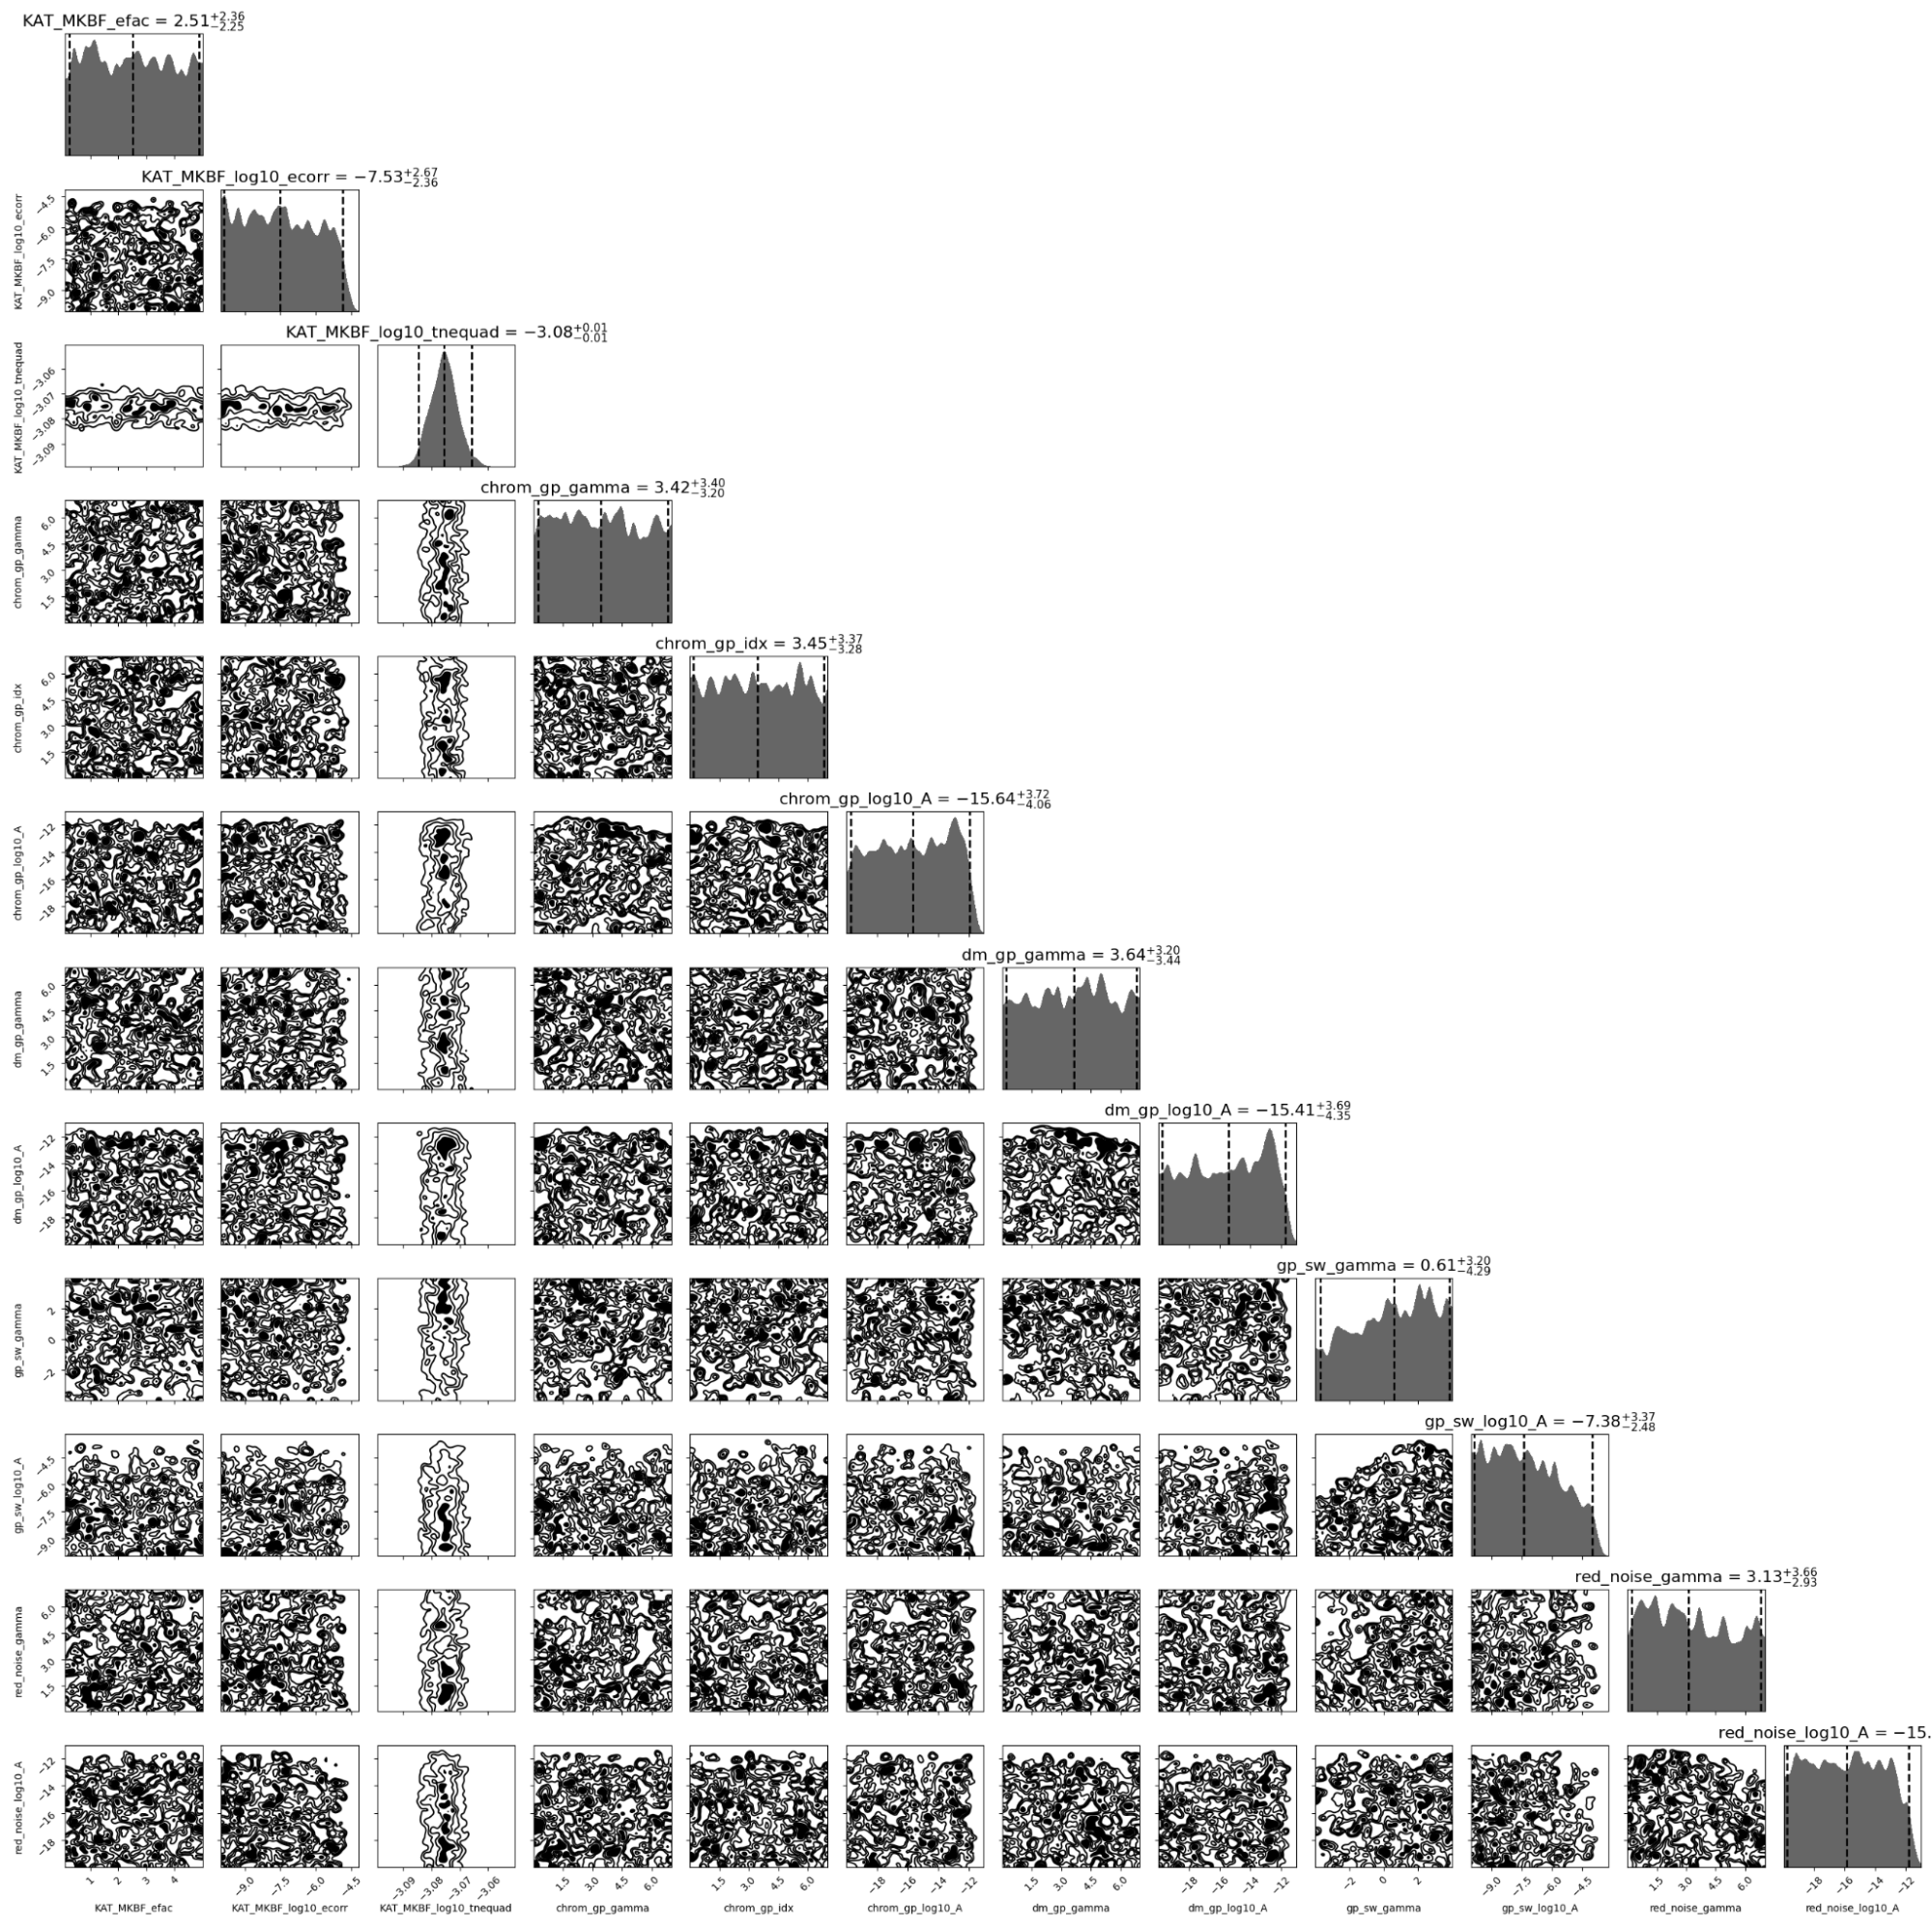
\includegraphics[width=\linewidth,height=0.38\textheight,keepaspectratio]{figures/image22.png}
      \caption{J1125-5825 (FD\_removed)}
      \label{fig:img1}
    \end{subfigure}
    &
    % Top-right
    \begin{subfigure}[b]{0.48\textwidth}
      \centering
      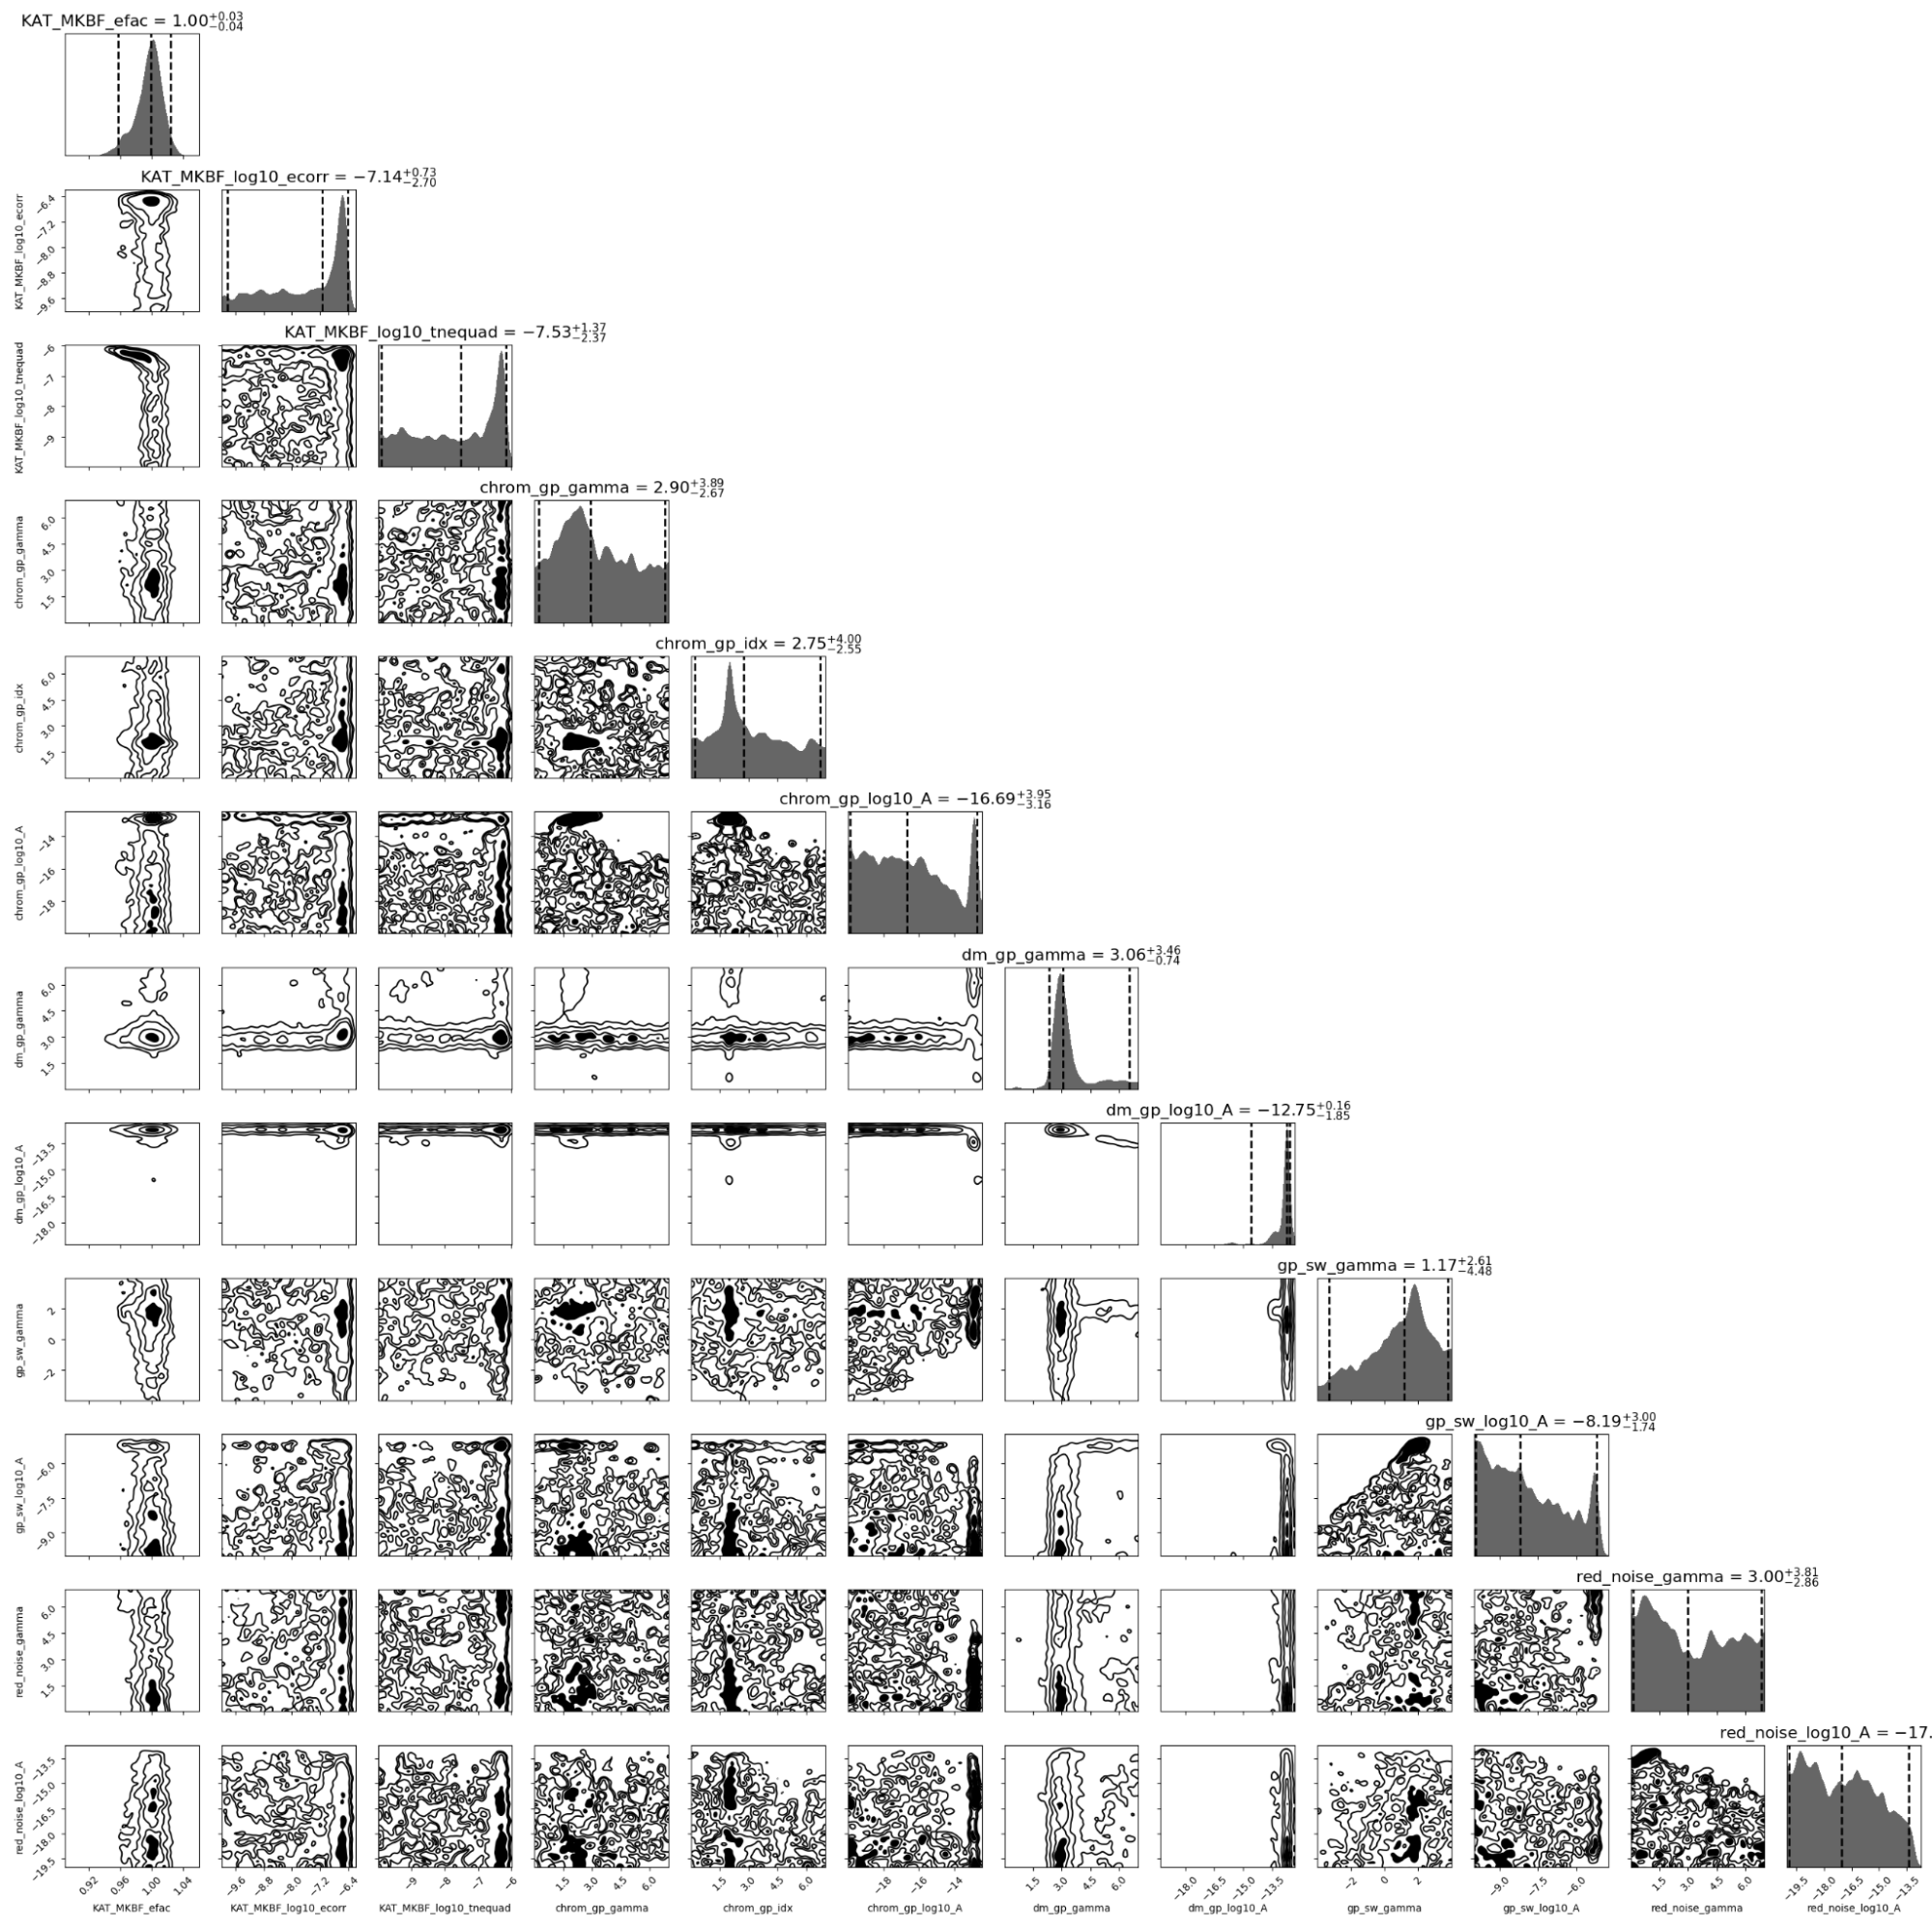
\includegraphics[width=\linewidth,height=0.38\textheight,keepaspectratio]{figures/image34.png}
      \caption{J1125-5825 (third\_pass)}
      \label{fig:img2}
    \end{subfigure}
    \\[8pt]
    % Bottom-left
    \begin{subfigure}[b]{0.48\textwidth}
      \centering
      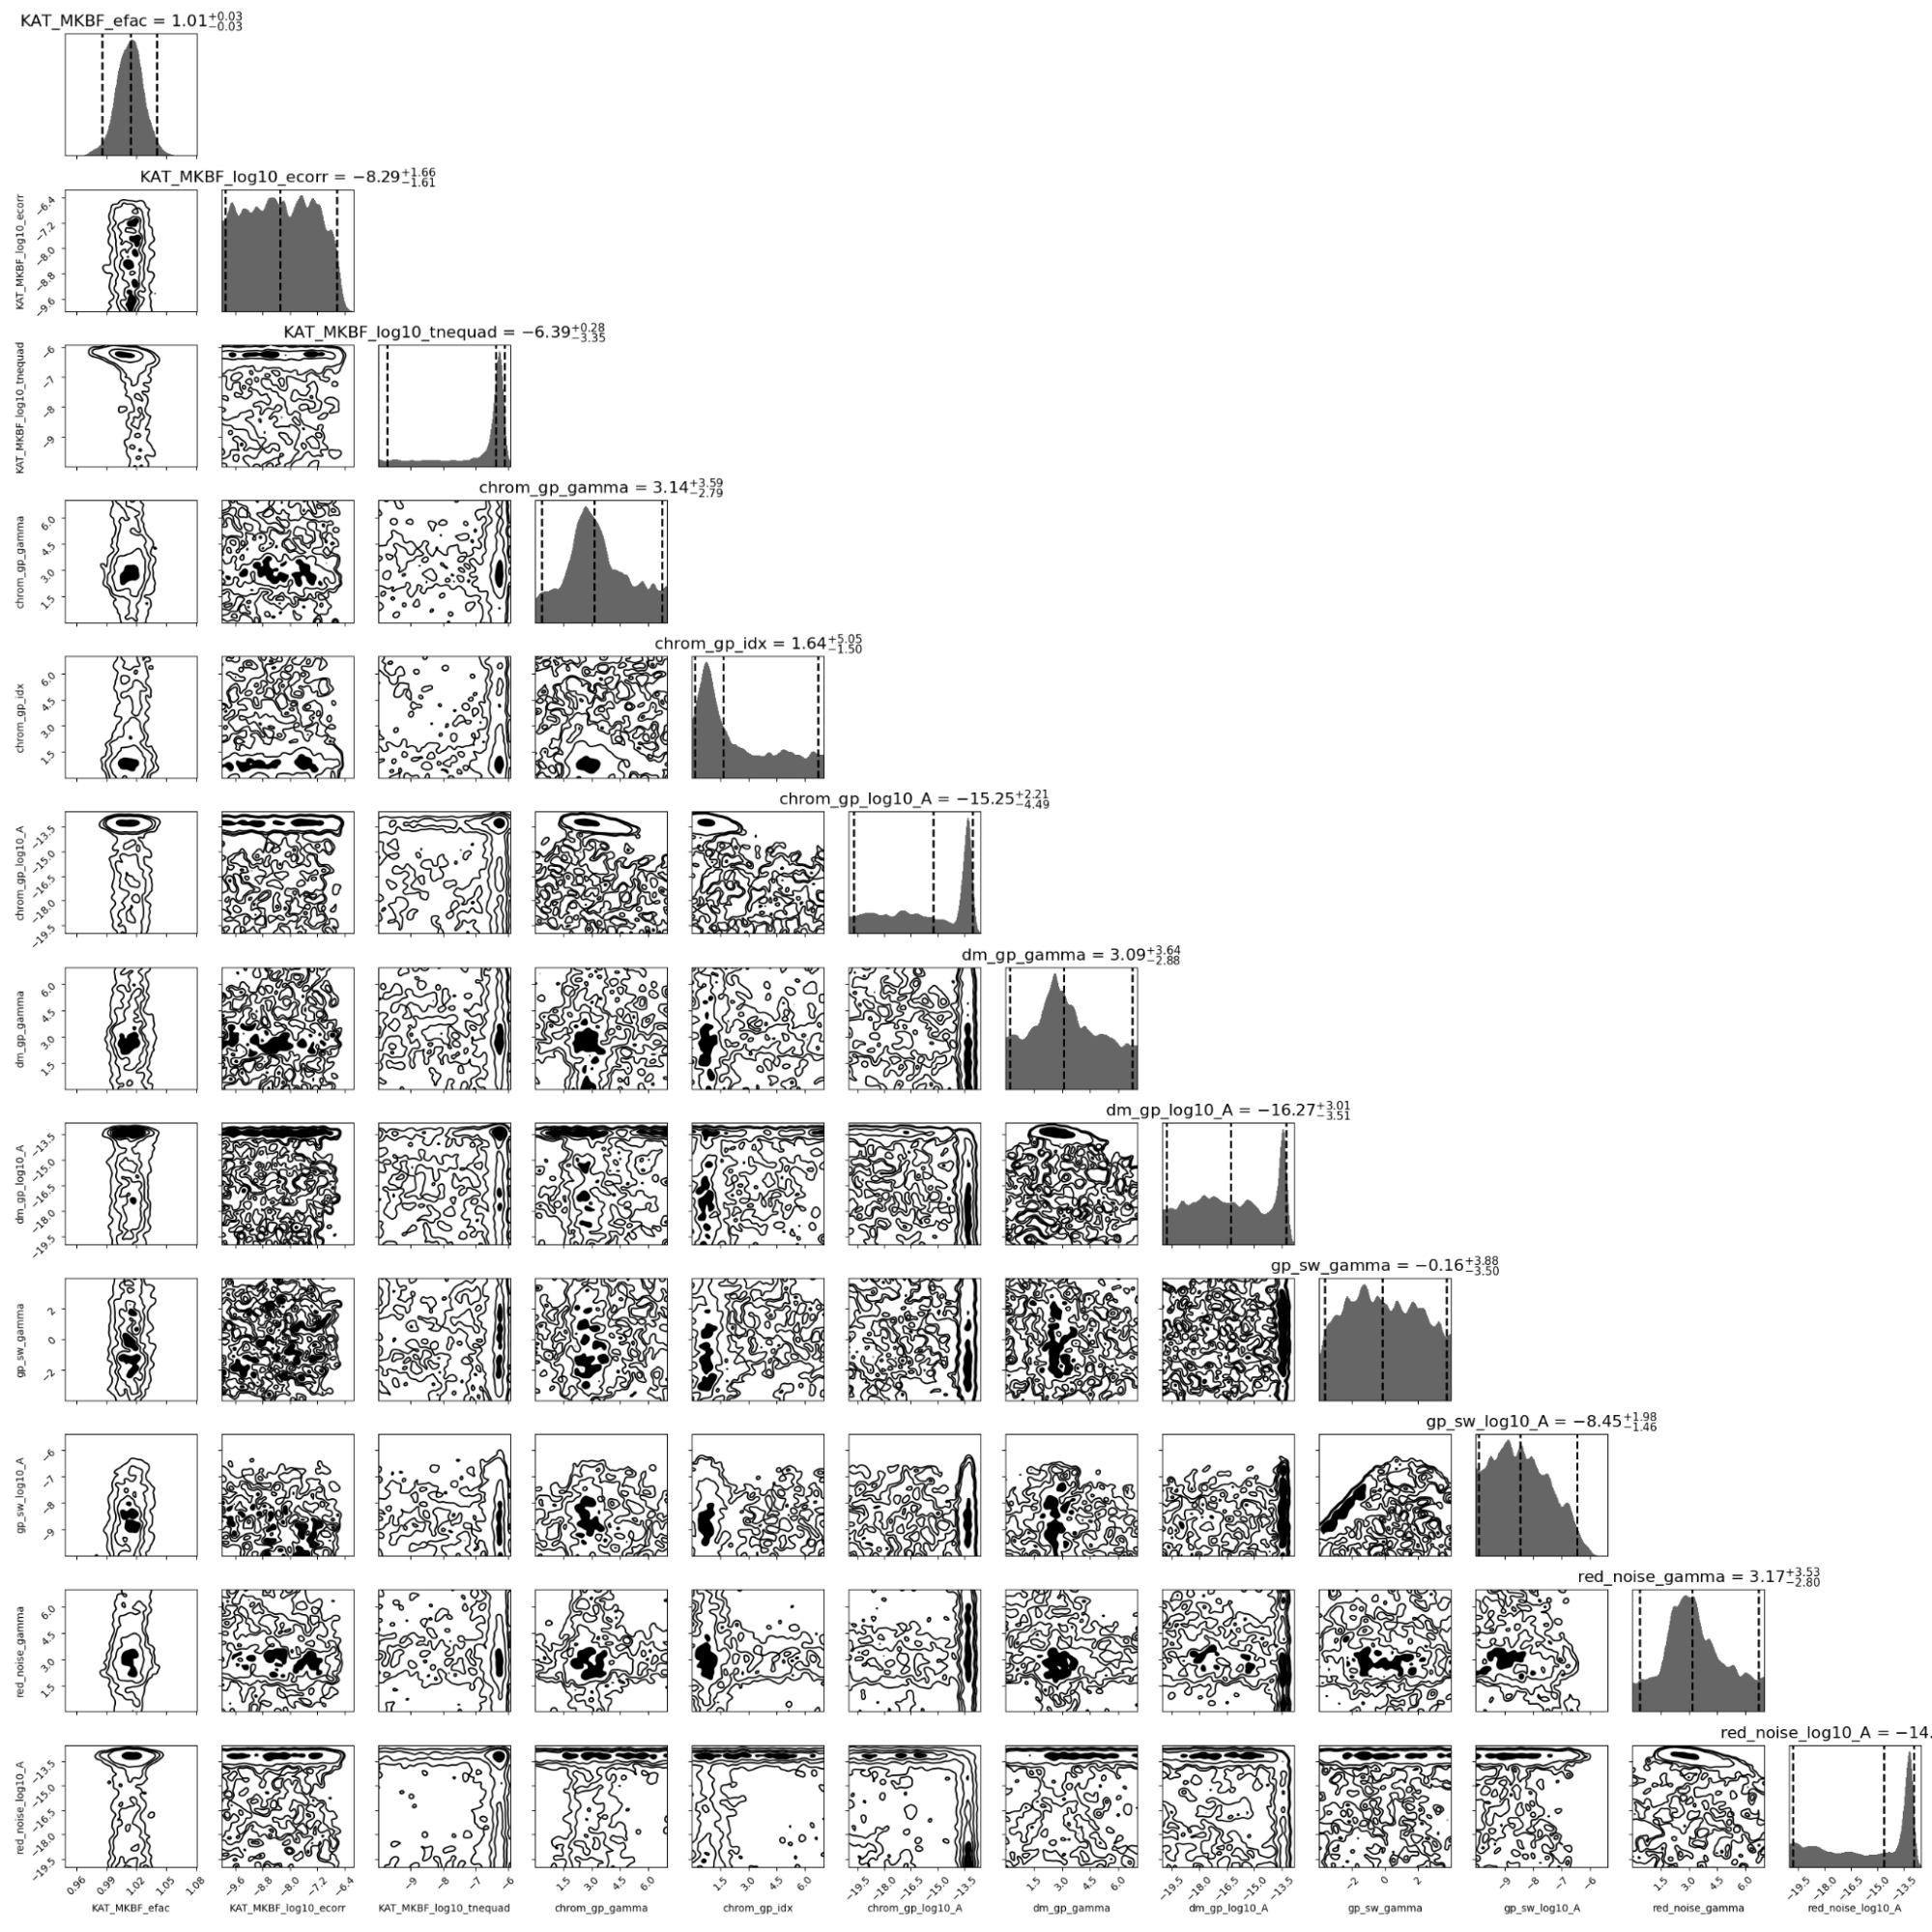
\includegraphics[width=\linewidth,height=0.38\textheight,keepaspectratio]{figures/image16.png}
      \caption{J1614-2230 (FD\_removed)}
      \label{fig:img3}
    \end{subfigure}
    &
    % Bottom-right
    \begin{subfigure}[b]{0.48\textwidth}
      \centering
      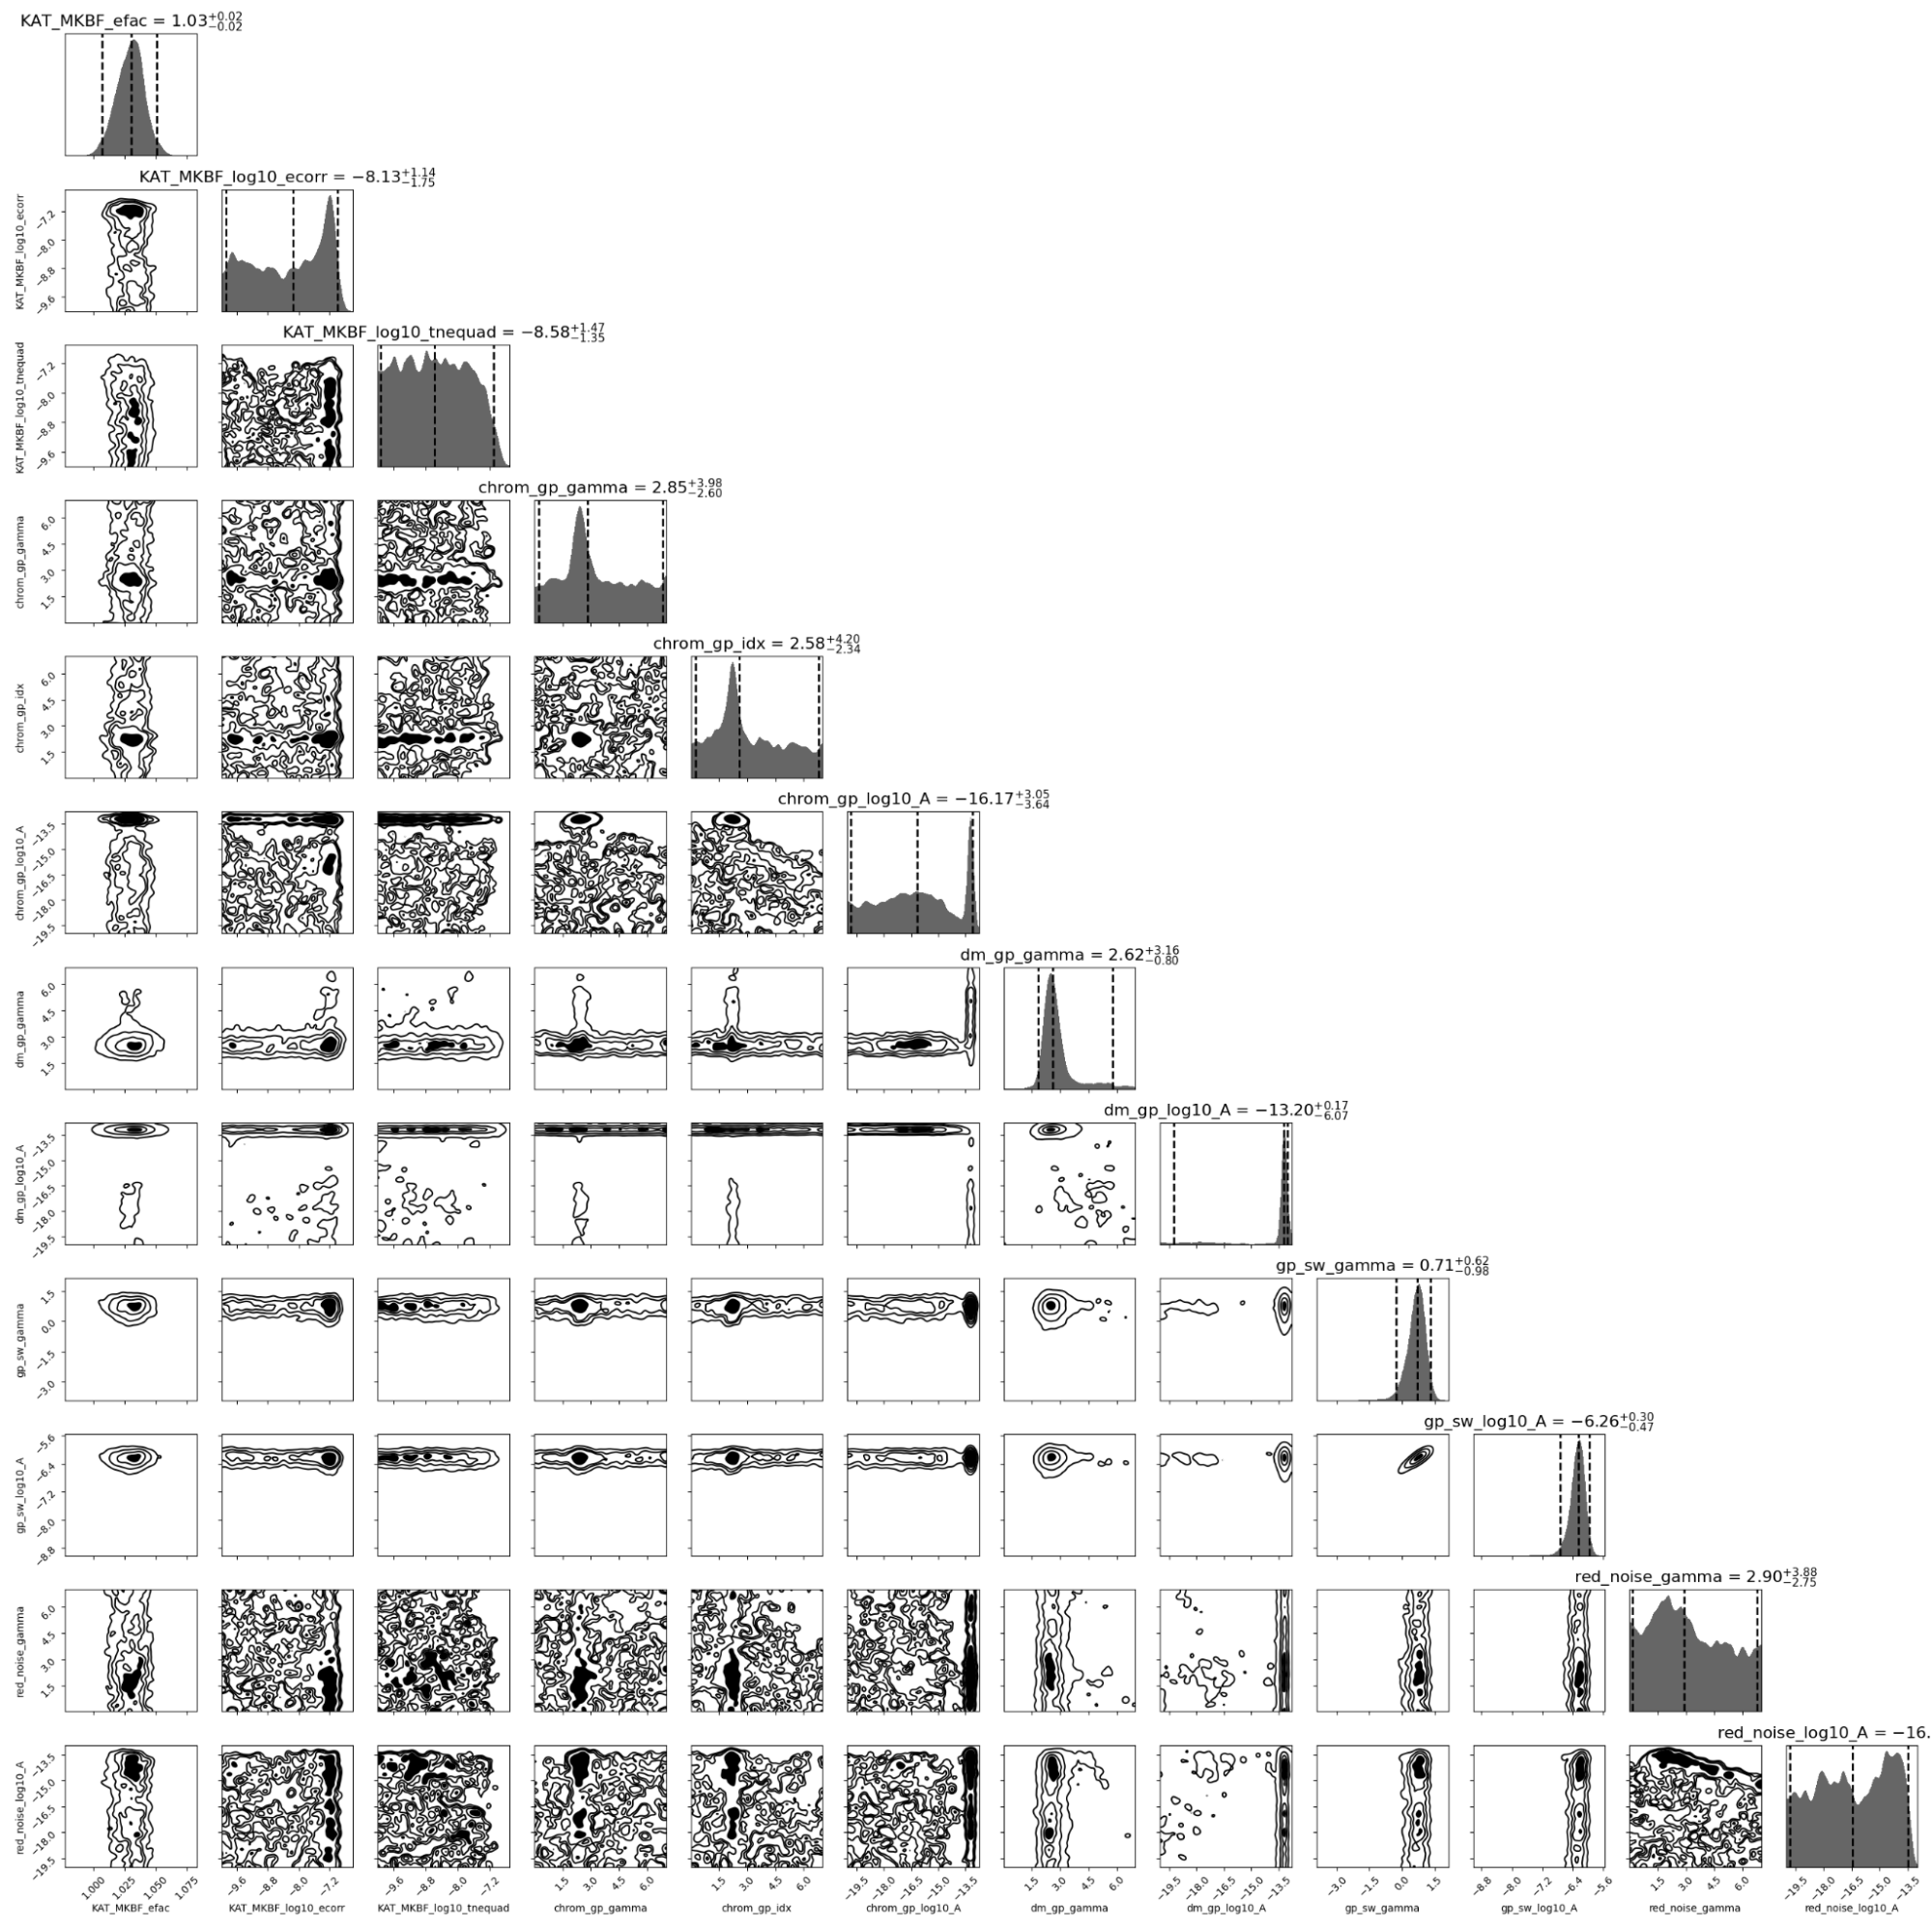
\includegraphics[width=\linewidth,height=0.38\textheight,keepaspectratio]{figures/image26.png}
      \caption{J1614-2230 (third\_pass)}
      \label{fig:img4}
    \end{subfigure}
    \\
  \end{tabular}
  \caption{Global caption describing the 2×2 panel.}
  \label{fig:2x2_noborder}
\end{figure}



For the "pooly behaving" pulsars, we see a completely different comparison. It's hard to summarize any specific comparative trends for these pulsars. But we can note the following worrying questions:

\begin{itemize}
  \item Why is the white noise so different? Is it absorbing any red noise which it shouldn't do?
  \item Intuitively, we would expect the DM or SW evidence to increase in these pulsars, as they should account for the unmodeled discrepancy between DM\_observed and DM\_predicted. However, in reality, the opposite occurs---the third\_pass dataset shows stronger evidence in almost all red noise posteriors.
\end{itemize}

\newpage

\section{Project 3: How does removing data in proximity to the sun affect the signal of the Gravitational Wave detected}


\subsection{Short intro: HD and Dipolar}
The Hellings--Downs (HD) curve is the quadrupolar angular correlation expected between pulsar timing residuals from an isotropic stochastic gravitational-wave background. A dipolar correlation instead produces a cos(\(\theta\))-like pattern and is characteristic of systematics that project onto the solar-system frame (for example ephemeris errors or poorly modelled solar wind). Extending the optimal-statistic discussion: comparing HD and dipole SNRs helps diagnose whether observed correlations follow the astrophysical quadrupole expectation or are dominated by systematics. However, as seen later in this analysis, Optimal statistics can conflate these especially at low angular seperations where they look similar, resulting in spuriously high SNRs.

(Maybe add a diagram?? didn't really find a good one)

\subsection{Aim and datasets}
This analysis aimed at testing how removing pulsar data within a certain angle of the Sun will affect the signal of the Gravitational Wave detected.

It presents 2 datasets, the real dataset (\texttt{third\_pass}), and the simulated dataset (created by Saurav, with only efac, sw, and gwb injected). For each of the datasets, I chose the noise models in 2 different ways: with and without Solar wind parameters.

\subsection{Simulated dataset results}
There are a few trends worth noting:

\begin{figure}[H]
  \centering
  % Row 1
  \begin{subfigure}[b]{0.48\textwidth}
    \centering
    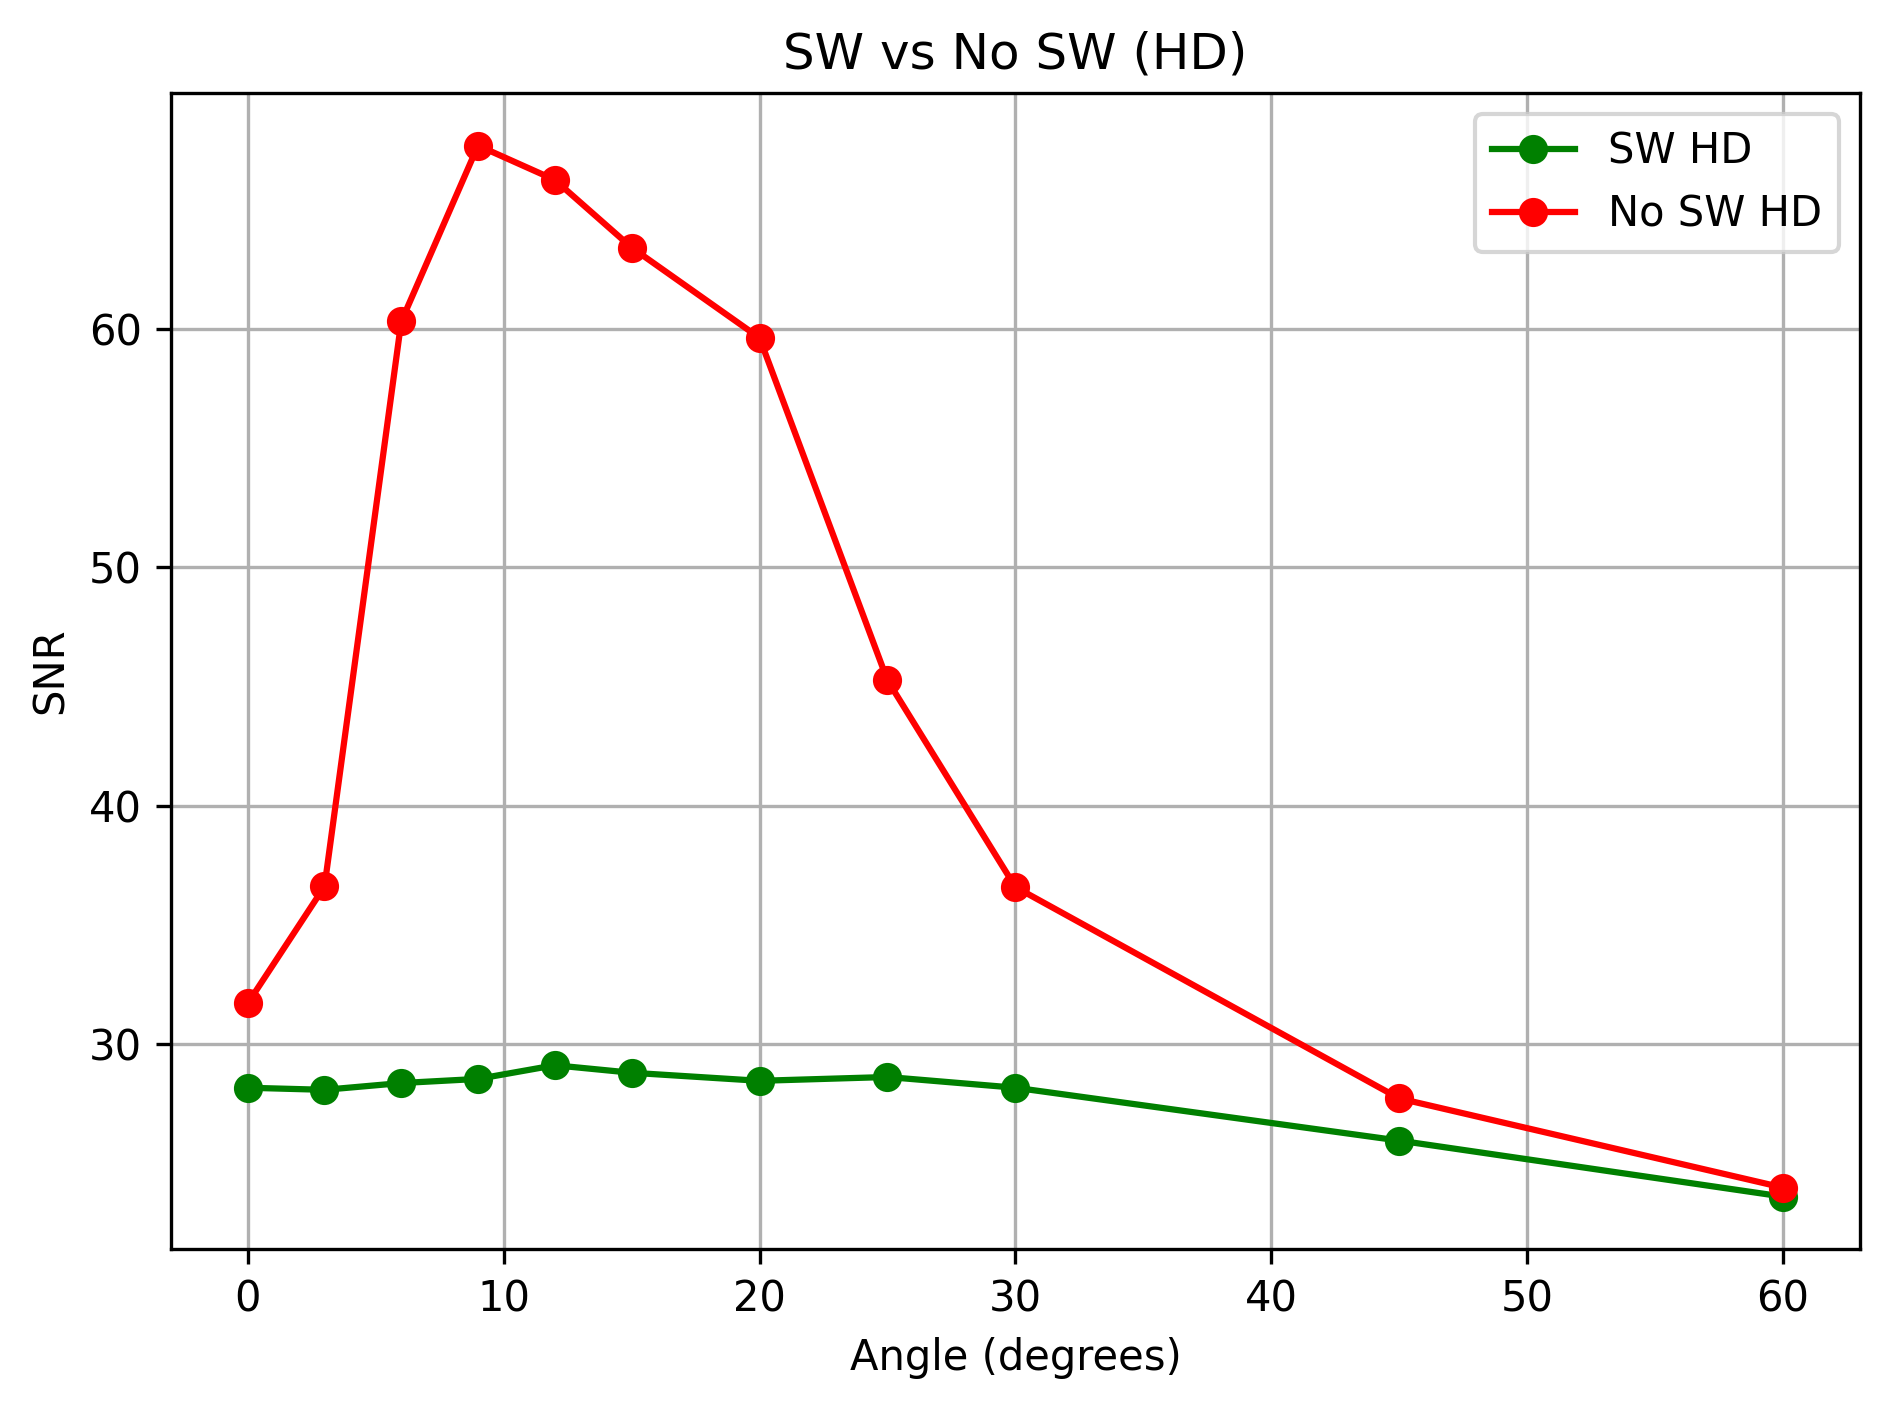
\includegraphics[width=\linewidth,height=0.38\textheight,keepaspectratio]{figures/image6.png}
    \caption{SNR\_HD with different noise models}
    \label{fig:img1}
  \end{subfigure}
  \hfill
  \begin{subfigure}[b]{0.48\textwidth}
    \centering
    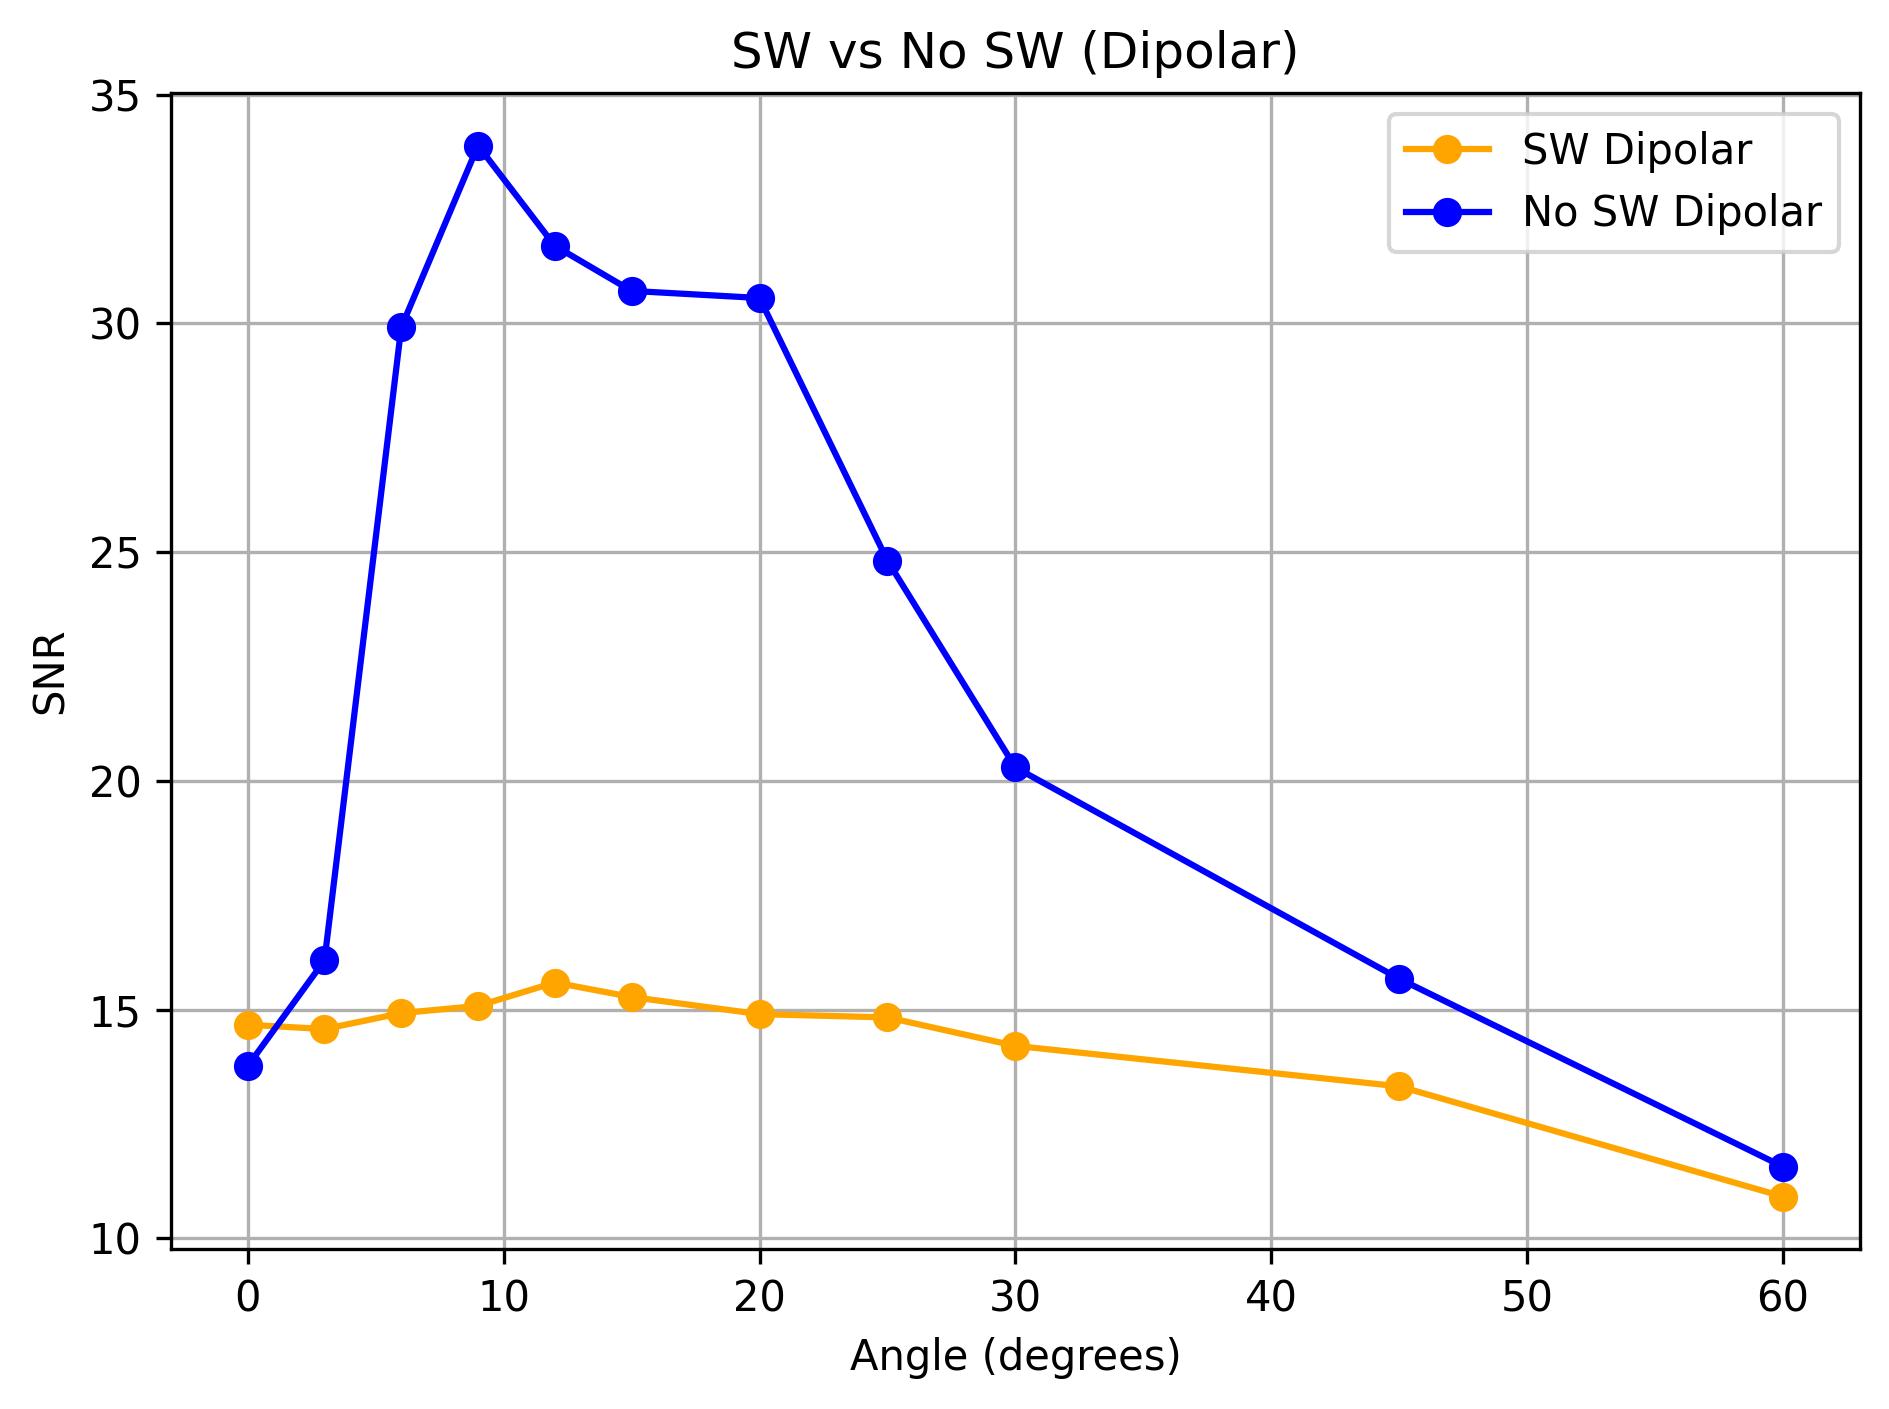
\includegraphics[width=\linewidth,height=0.38\textheight,keepaspectratio]{figures/image24.png}
    \caption{SNR\_dipolar with different noise models}
    \label{fig:img2}
  \end{subfigure}

  \vspace{8pt} 

  % Row 2
  \begin{subfigure}[b]{0.48\textwidth}
    \centering
    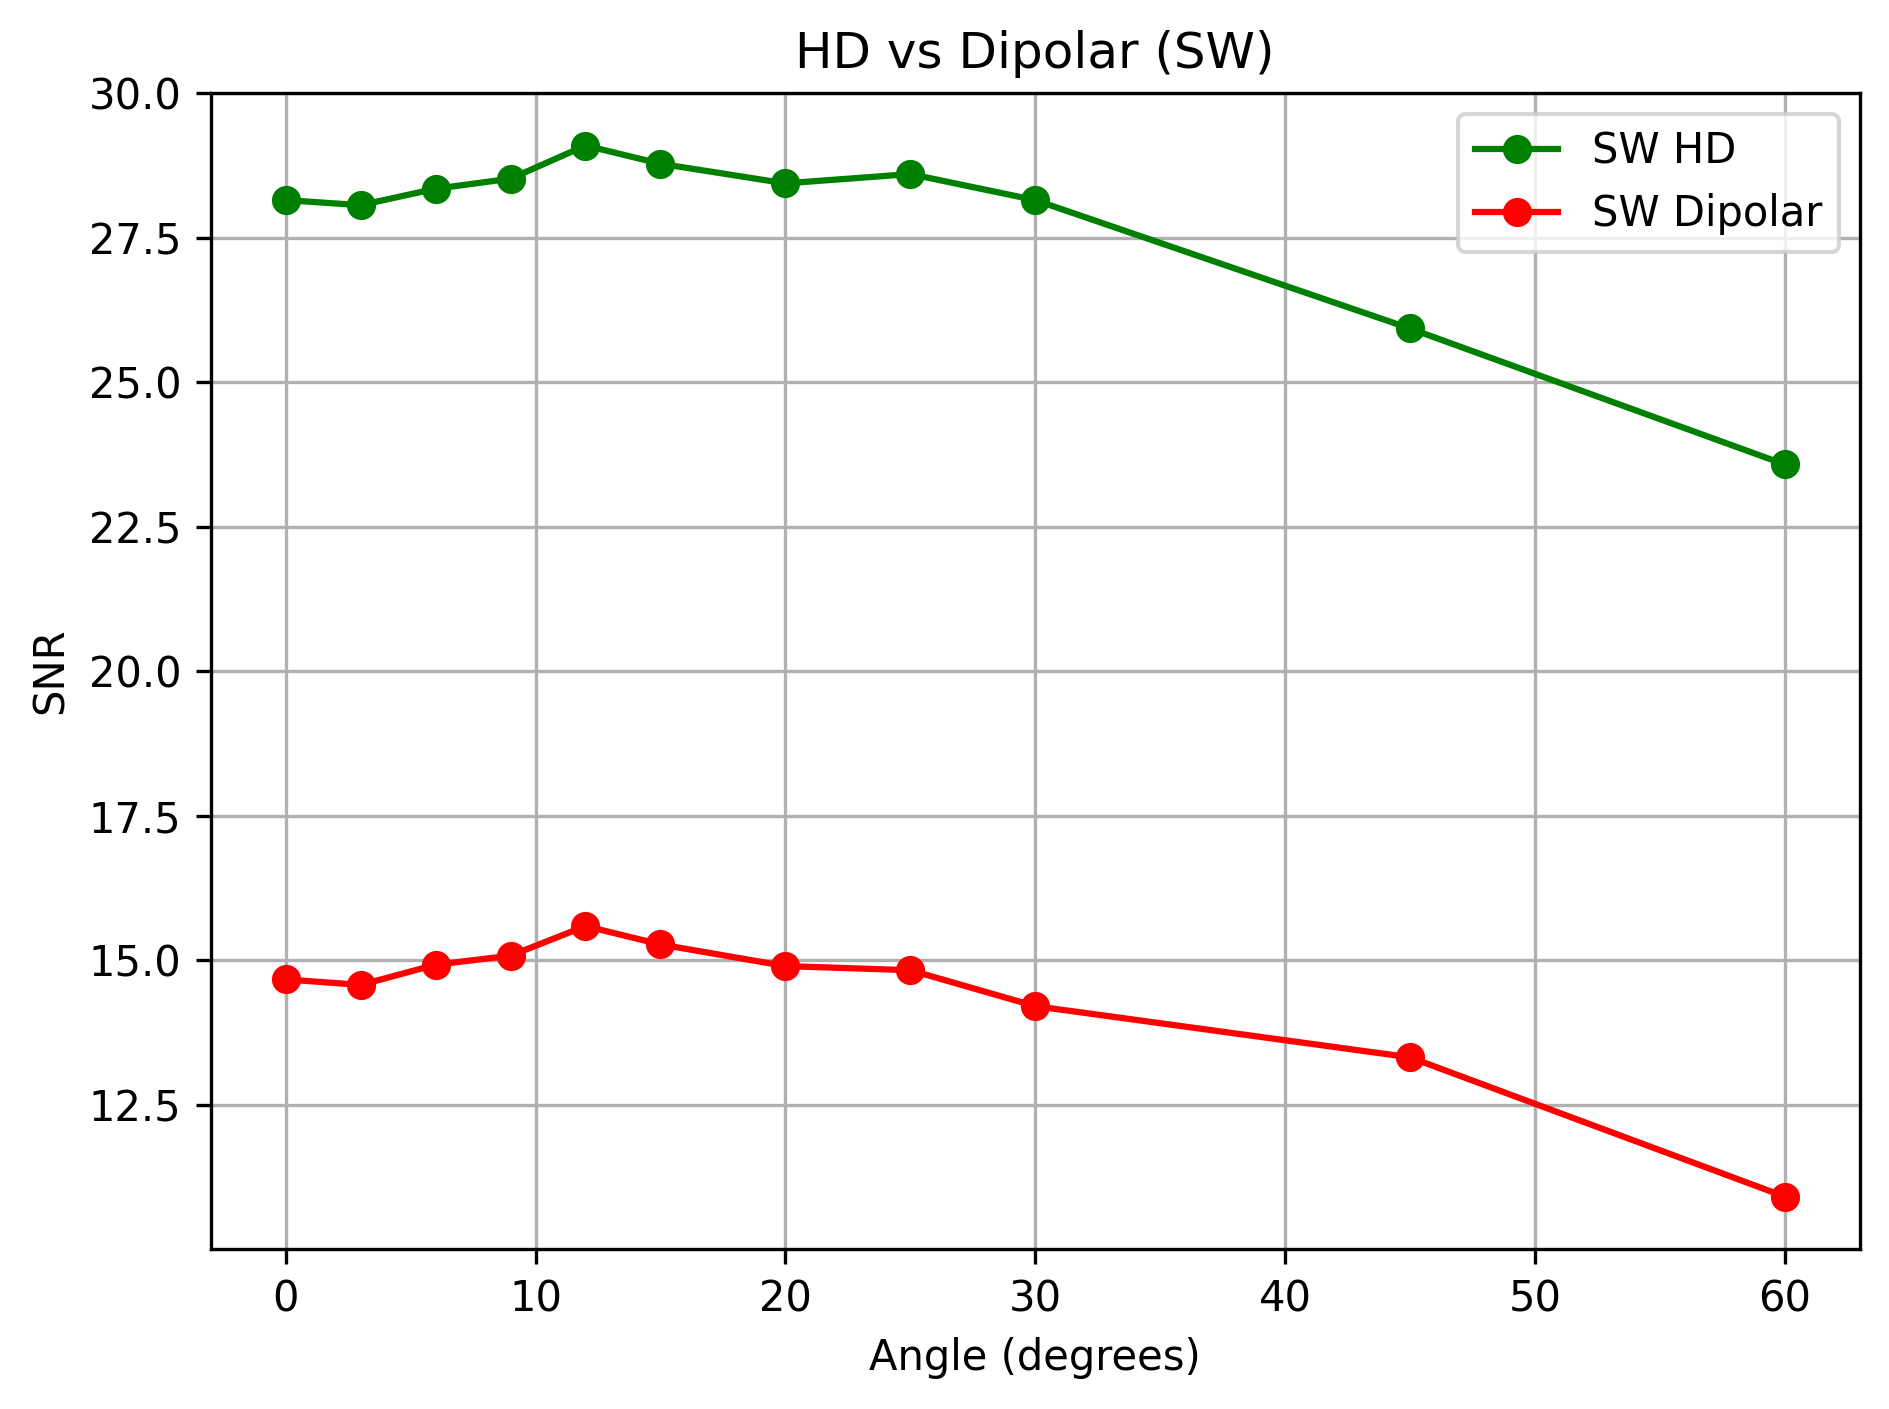
\includegraphics[width=\linewidth,height=0.38\textheight,keepaspectratio]{figures/image7.png}
    \caption{SNR\_HD and SNR\_dipolar with SW model}
    \label{fig:img3}
  \end{subfigure}
  \hfill
  \begin{subfigure}[b]{0.48\textwidth}
    \centering
    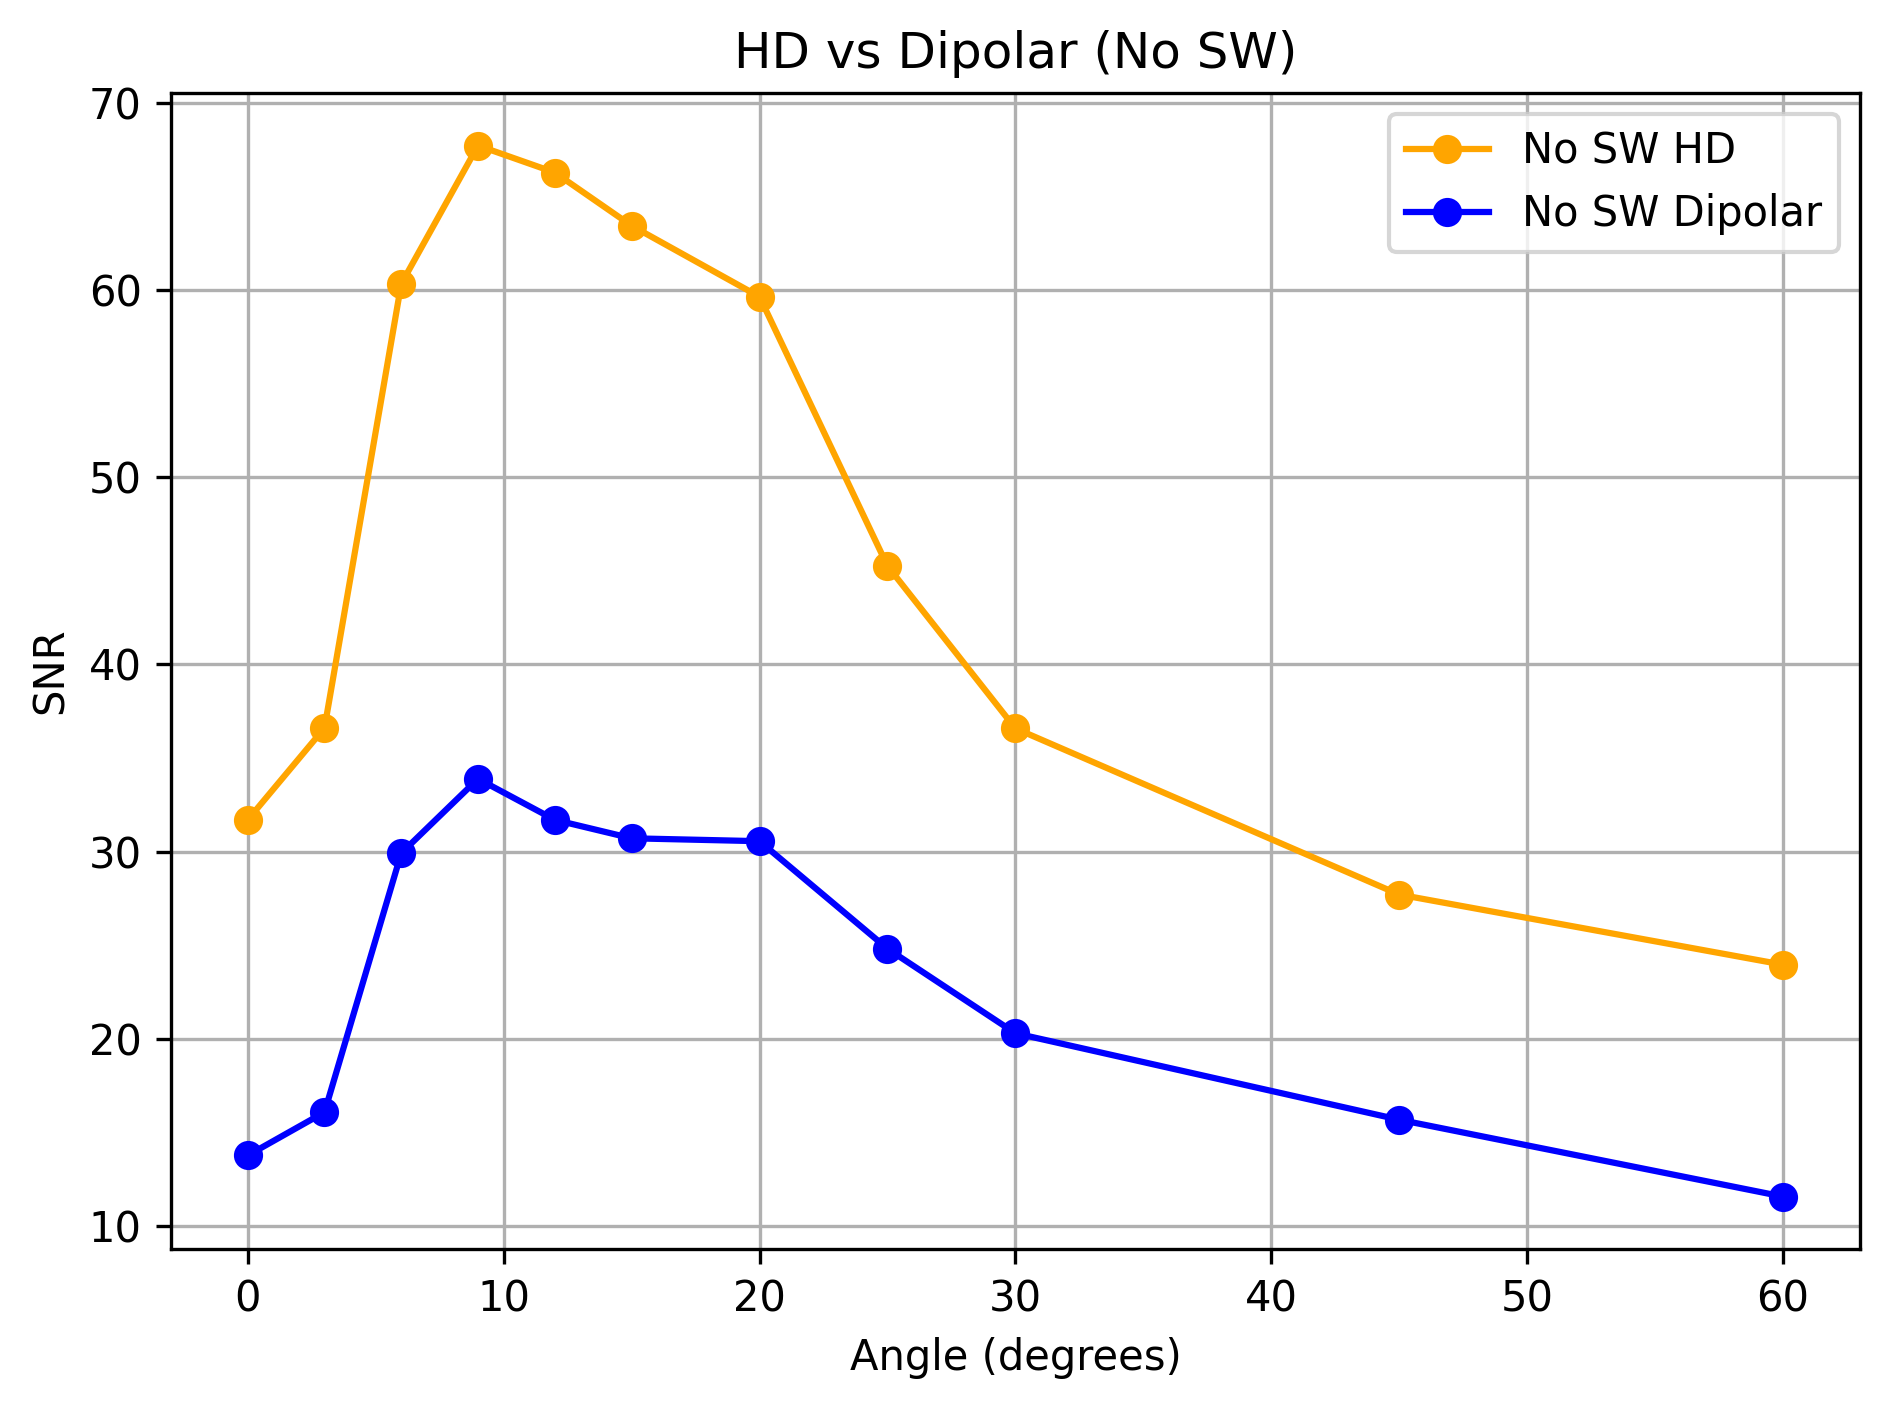
\includegraphics[width=\linewidth,height=0.38\textheight,keepaspectratio]{figures/image5.png}
    \caption{SNR\_HD and SNR\_dipolar with no\_SW model}
    \label{fig:img4}
  \end{subfigure}

  \caption{Global caption describing the 2×2 panel.}
  \label{fig:2x2_noborder}
\end{figure}


\begin{itemize}
  \item For the SW dataset, the SNR of the Hellings-Downs (HD) correlation pattern remains steady until around 30 degrees (the peak is at 12 degrees cut, though not by much). This pattern is rather straightforward to explain
    \begin{itemize}
      \item At sufficiently large angles, not enough data remains, decreasing the sensitivity of the simulated array, hence a decrease in SNR
      \item (I'm not sure about this) There is no significant increase in SNR for any cuts, as the noise injected is well understood and well modelled by our current solar wind modelling, hence we don't expect deleting data close to the sun to improve SNR significantly.
    \end{itemize}
  \item For the no\_SW dataset, SNR(HD) seems to be always higher than the SW dataset. Though the numbers might be surprising, the observation can be explained by visually examining the plots.
    \begin{itemize}
      \item The pattern of the datapoints(bins) deviates significantly from the theoretical HD curve. This can be seen as a consequence of unmodelled solar wind effects, producing a stronger dipolar signature (evident in the trend later discussed), which becomes absorbed by the HD SNR. (But it's not a perfect Dipolar pattern as well? Perhaps it is a mixture of both?)
    \end{itemize}
\end{itemize}

\begin{figure}[H]
  \centering
  % Left panel
  \begin{subfigure}[b]{0.48\textwidth}
    \centering
    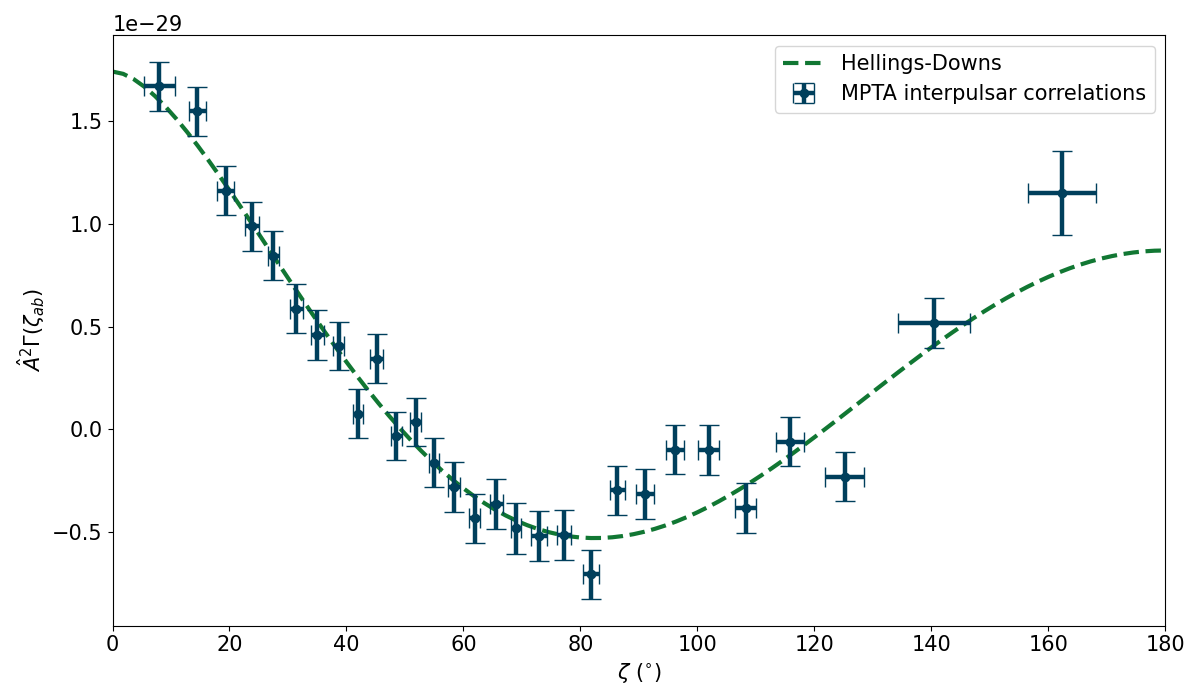
\includegraphics[width=\linewidth,height=0.42\textheight,keepaspectratio]{figures/image31.png}
    \caption{HD plot with normal noise modeling}
    \label{fig:left}
  \end{subfigure}
  \hfill
  % Right panel
  \begin{subfigure}[b]{0.48\textwidth}
    \centering
    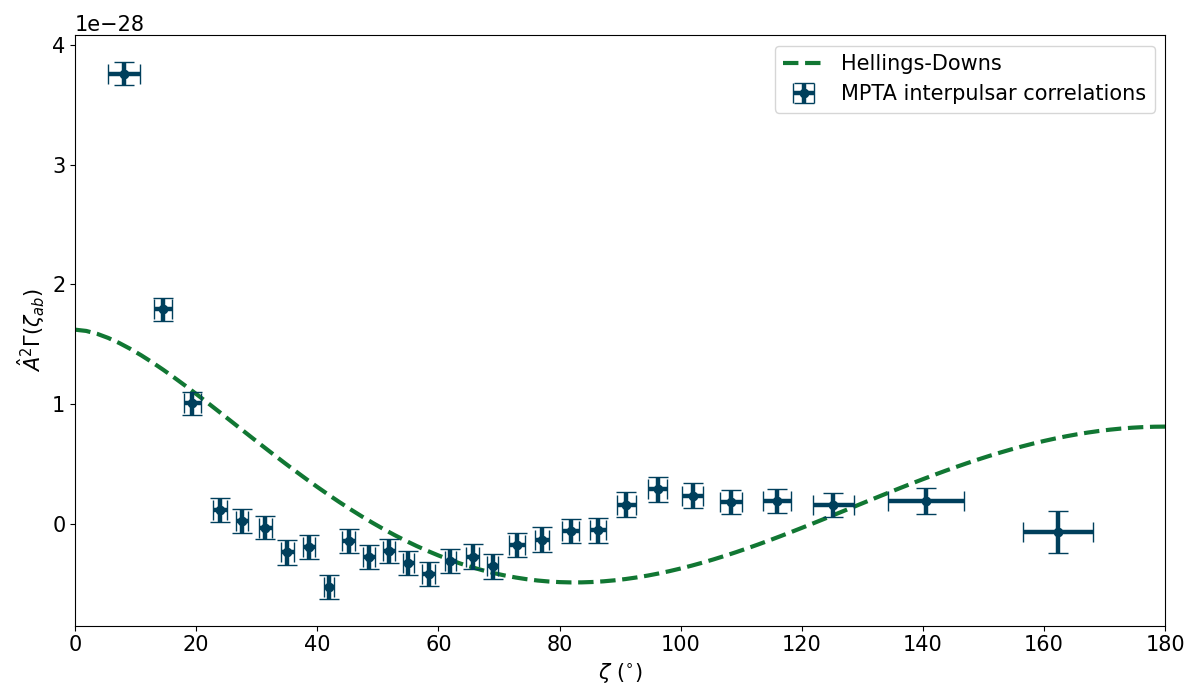
\includegraphics[width=\linewidth,height=0.42\textheight,keepaspectratio]{figures/image20.png}
    \caption{HD plot with no SW noise modelling}
    \label{fig:right}
  \end{subfigure}

  \caption{Global caption describing the 1×2 comparison.}
  \label{fig:1x2_noborder}
\end{figure}


The above trends are rather predicted/well explained. A more interesting observation is the correlation between the HD and Dipolar SNR for both the SW and no\_SW datasets. The similarity of the 2 patterns is easily seen in the plots shown above. So I decided to compute the Pearson correlation coefficient for them. The following results were obtained:

The SNR of HD and Dipolar for the same dataset almost perfectly imitates a linear relationship.

It is totally expected that they will be absorbed somewhat by each other, but is it really expected that there is such a perfectly linear correlation?

Is this a natural consequence of the Opstat algorithm when the dataset is ideal (why is it not reflected in the real dataset, is it only because the dataset is ideal and well modelled?), or does it suggest other issues?

Pearson r (SW HD vs SW Dipolar) = 0.985, p = 1.08e-16

Pearson r (No SW HD vs No SW Dipolar) = 0.982, p = 7.14e-16

\subsection{Real dataset results}
For the real data:

\begin{itemize}
  \item The same trends are not observed with the real dataset. However, the value of the statistics produced for the real dataset is questionable. The datapoints for the normal (SW) dataset look strongly dipolar, and are not much different from the no\_SW version. This may suggest that this current preliminary model doesn't model solar wind that well or there are other processing required (e.g. removal of points etc.)
  \item Correlation values for the real data:
    \begin{itemize}
      \item Pearson \(r\) (SW HD vs No SW HD) = 0.812, \(p = 4.46\times10^{-6}\)
      \item Pearson \(r\) (SW Dipolar vs No SW Dipolar) = 0.566, \(p = 6.05\times10^{-3}\)
      \item Pearson \(r\) (SW HD vs SW Dipolar) = 0.154, \(p = 0.495\)
      \item Pearson \(r\) (No SW HD vs No SW Dipolar) = 0.959, \(p = 2.29\times10^{-12}\)
    \end{itemize}
\end{itemize}


\begin{figure}[H]
  \centering
  % Left panel
  \begin{subfigure}[b]{0.48\textwidth}
    \centering
    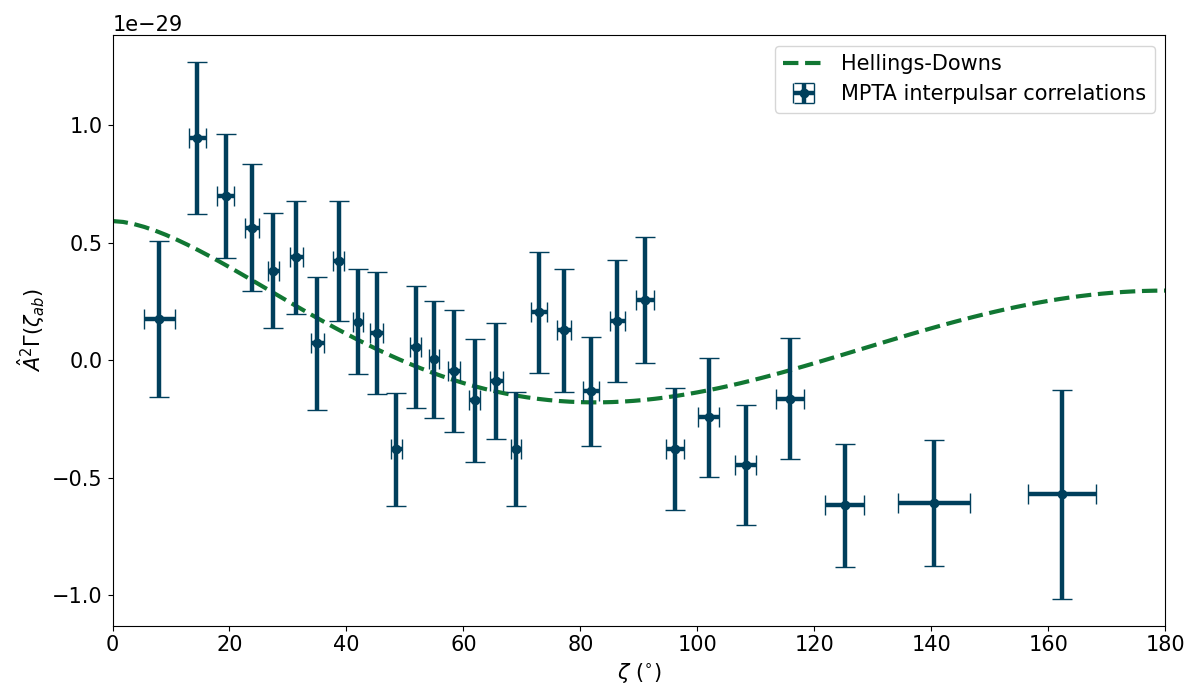
\includegraphics[width=\linewidth,height=0.42\textheight,keepaspectratio]{figures/image8.png}
    \caption{HD plot with normal noise modeling}
    \label{fig:left}
  \end{subfigure}
  \hfill
  % Right panel
  \begin{subfigure}[b]{0.48\textwidth}
    \centering
    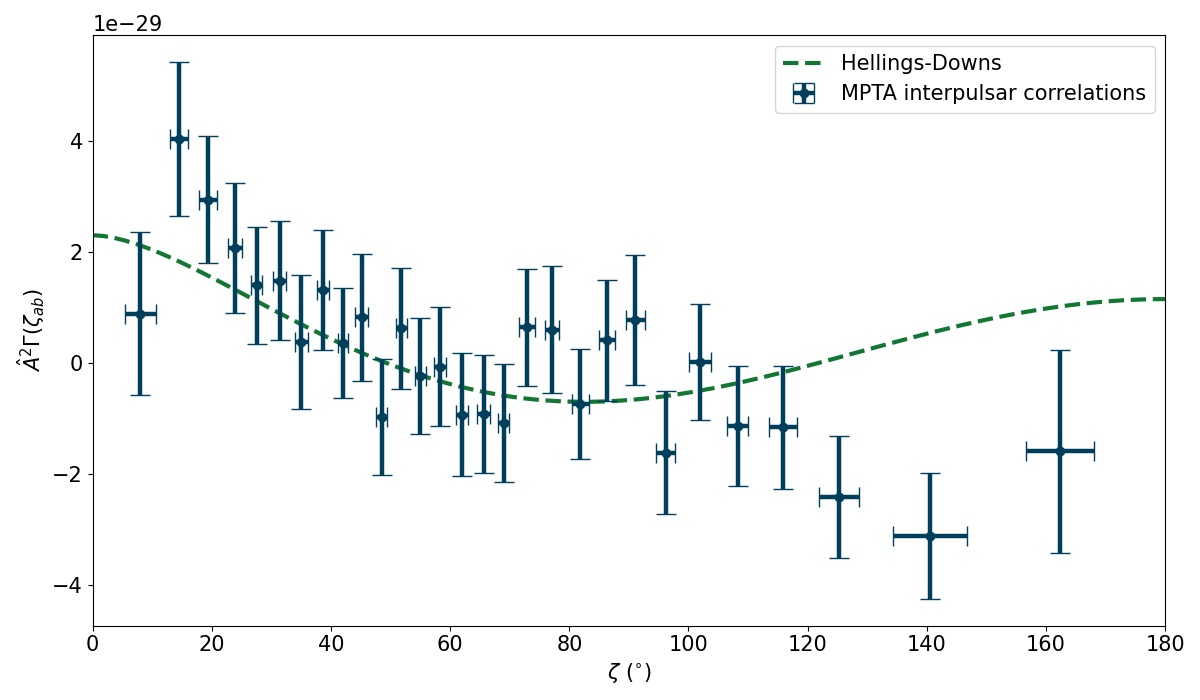
\includegraphics[width=\linewidth,height=0.42\textheight,keepaspectratio]{figures/image15.png}
    \caption{HD plot with no SW noise modelling}
    \label{fig:right}
  \end{subfigure}

  \caption{Global caption describing the 1×2 comparison.}
  \label{fig:1x2_noborder}
\end{figure}



I haven't analysed the trends for the real data that much due to the questionable reliability of the statistics mentioned above. The only interesting plots that I looked at were the 9 degree cut with SW modelling, the HD SNR was the highest and the Dipolar SNR was the lowest. However, examining the plot the datapoints just seem like a mess and look like random jitter rather than any identifiable patterns.


\begin{figure}[H]
  \centering
  % Row 1
  \begin{subfigure}[b]{0.48\textwidth}
    \centering
    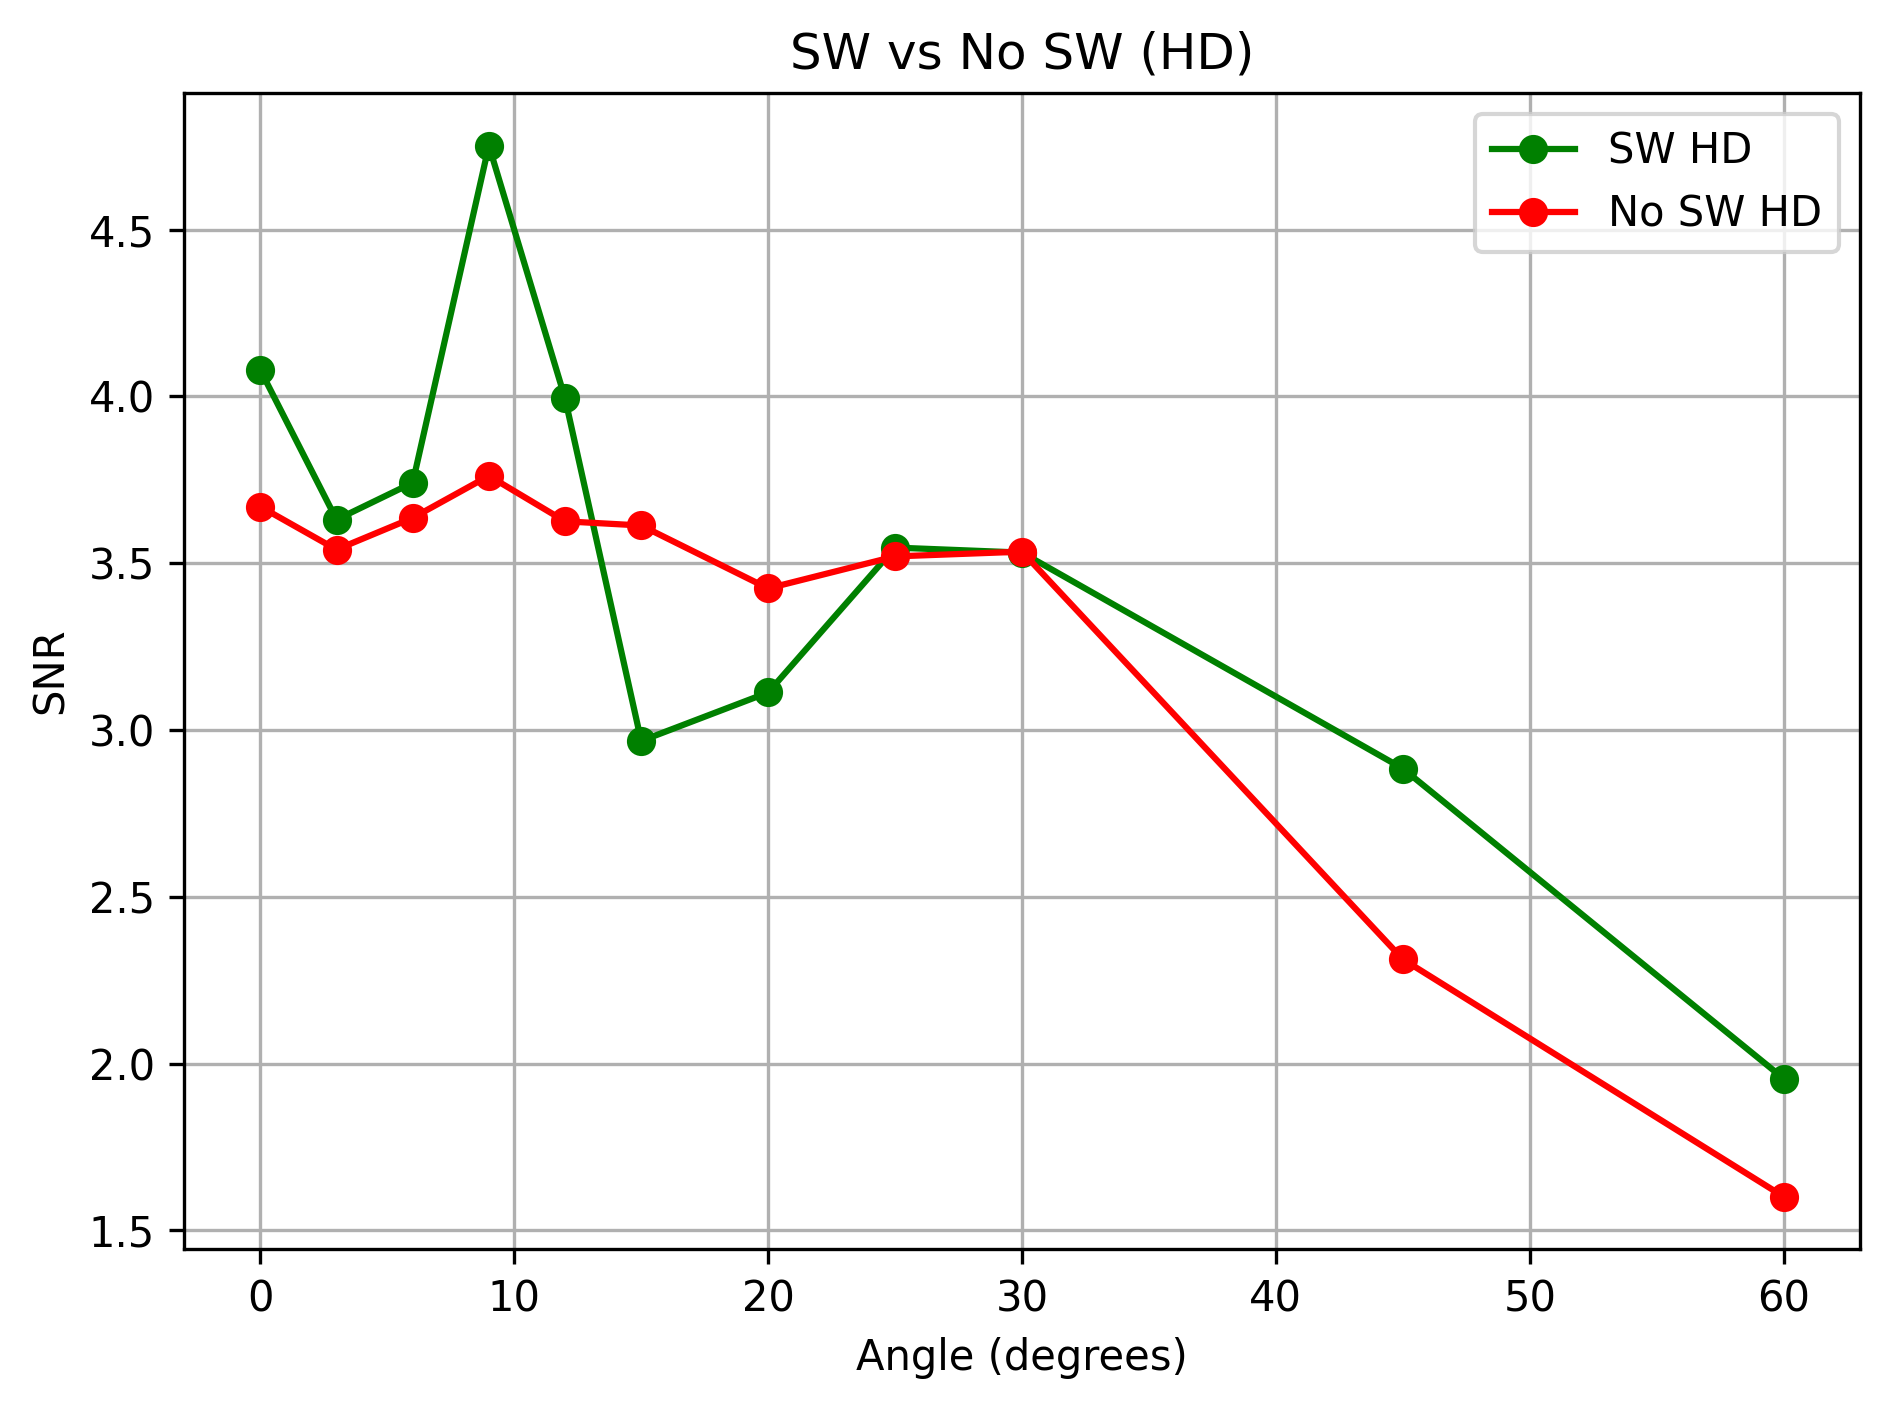
\includegraphics[width=\linewidth,height=0.38\textheight,keepaspectratio]{figures/image27.png}
    \caption{SNR\_HD with different noise models}
    \label{fig:img1}
  \end{subfigure}
  \hfill
  \begin{subfigure}[b]{0.48\textwidth}
    \centering
    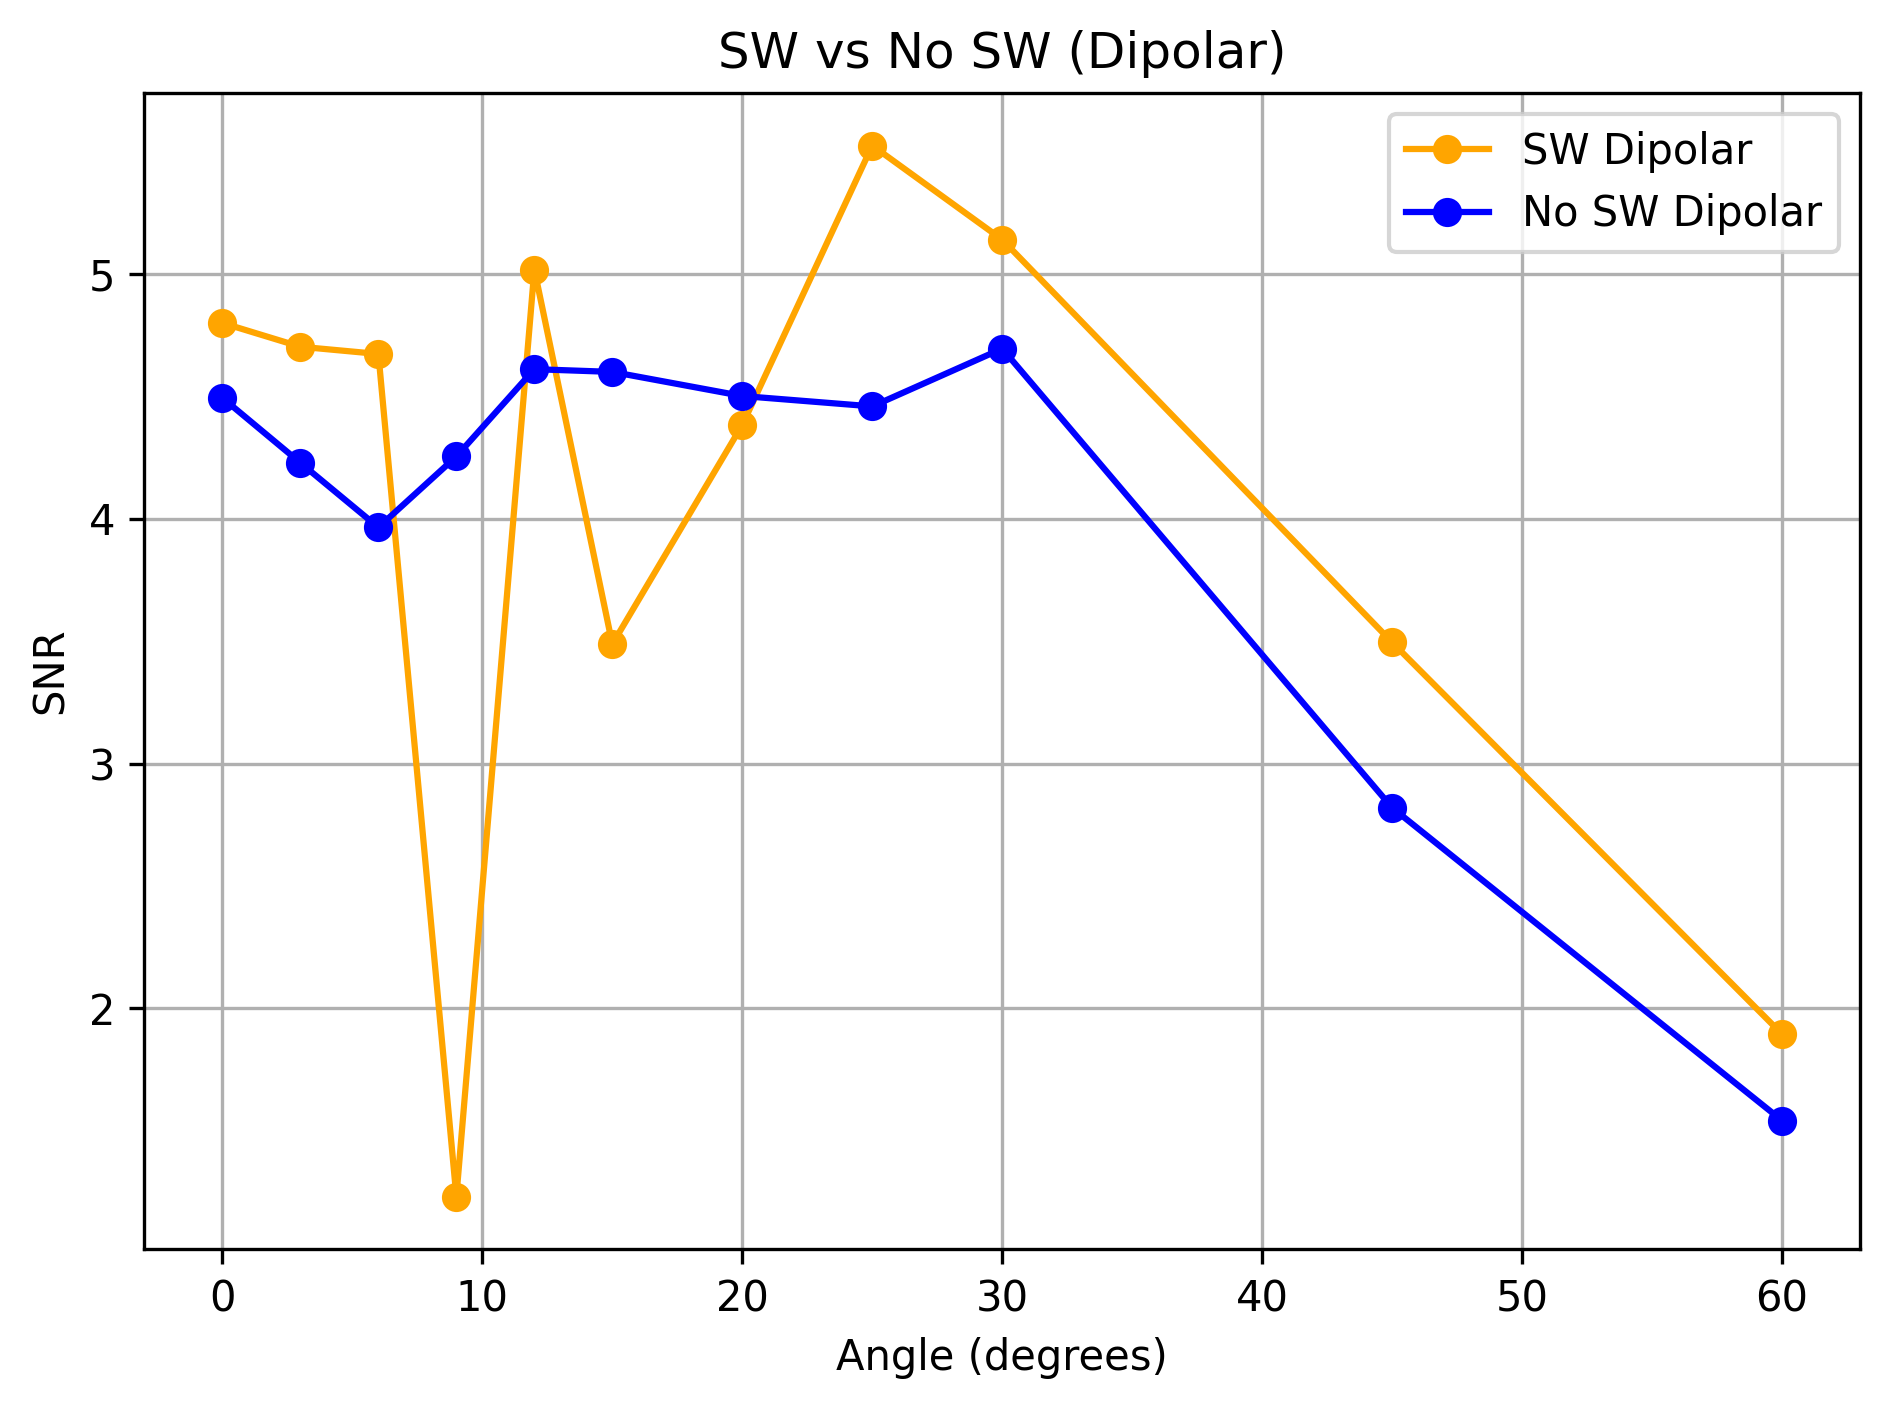
\includegraphics[width=\linewidth,height=0.38\textheight,keepaspectratio]{figures/image17.png}
    \caption{SNR\_dipolar with different noise models}
    \label{fig:img2}
  \end{subfigure}

  \vspace{8pt} 
  
  % Row 2
  \begin{subfigure}[b]{0.48\textwidth}
    \centering
    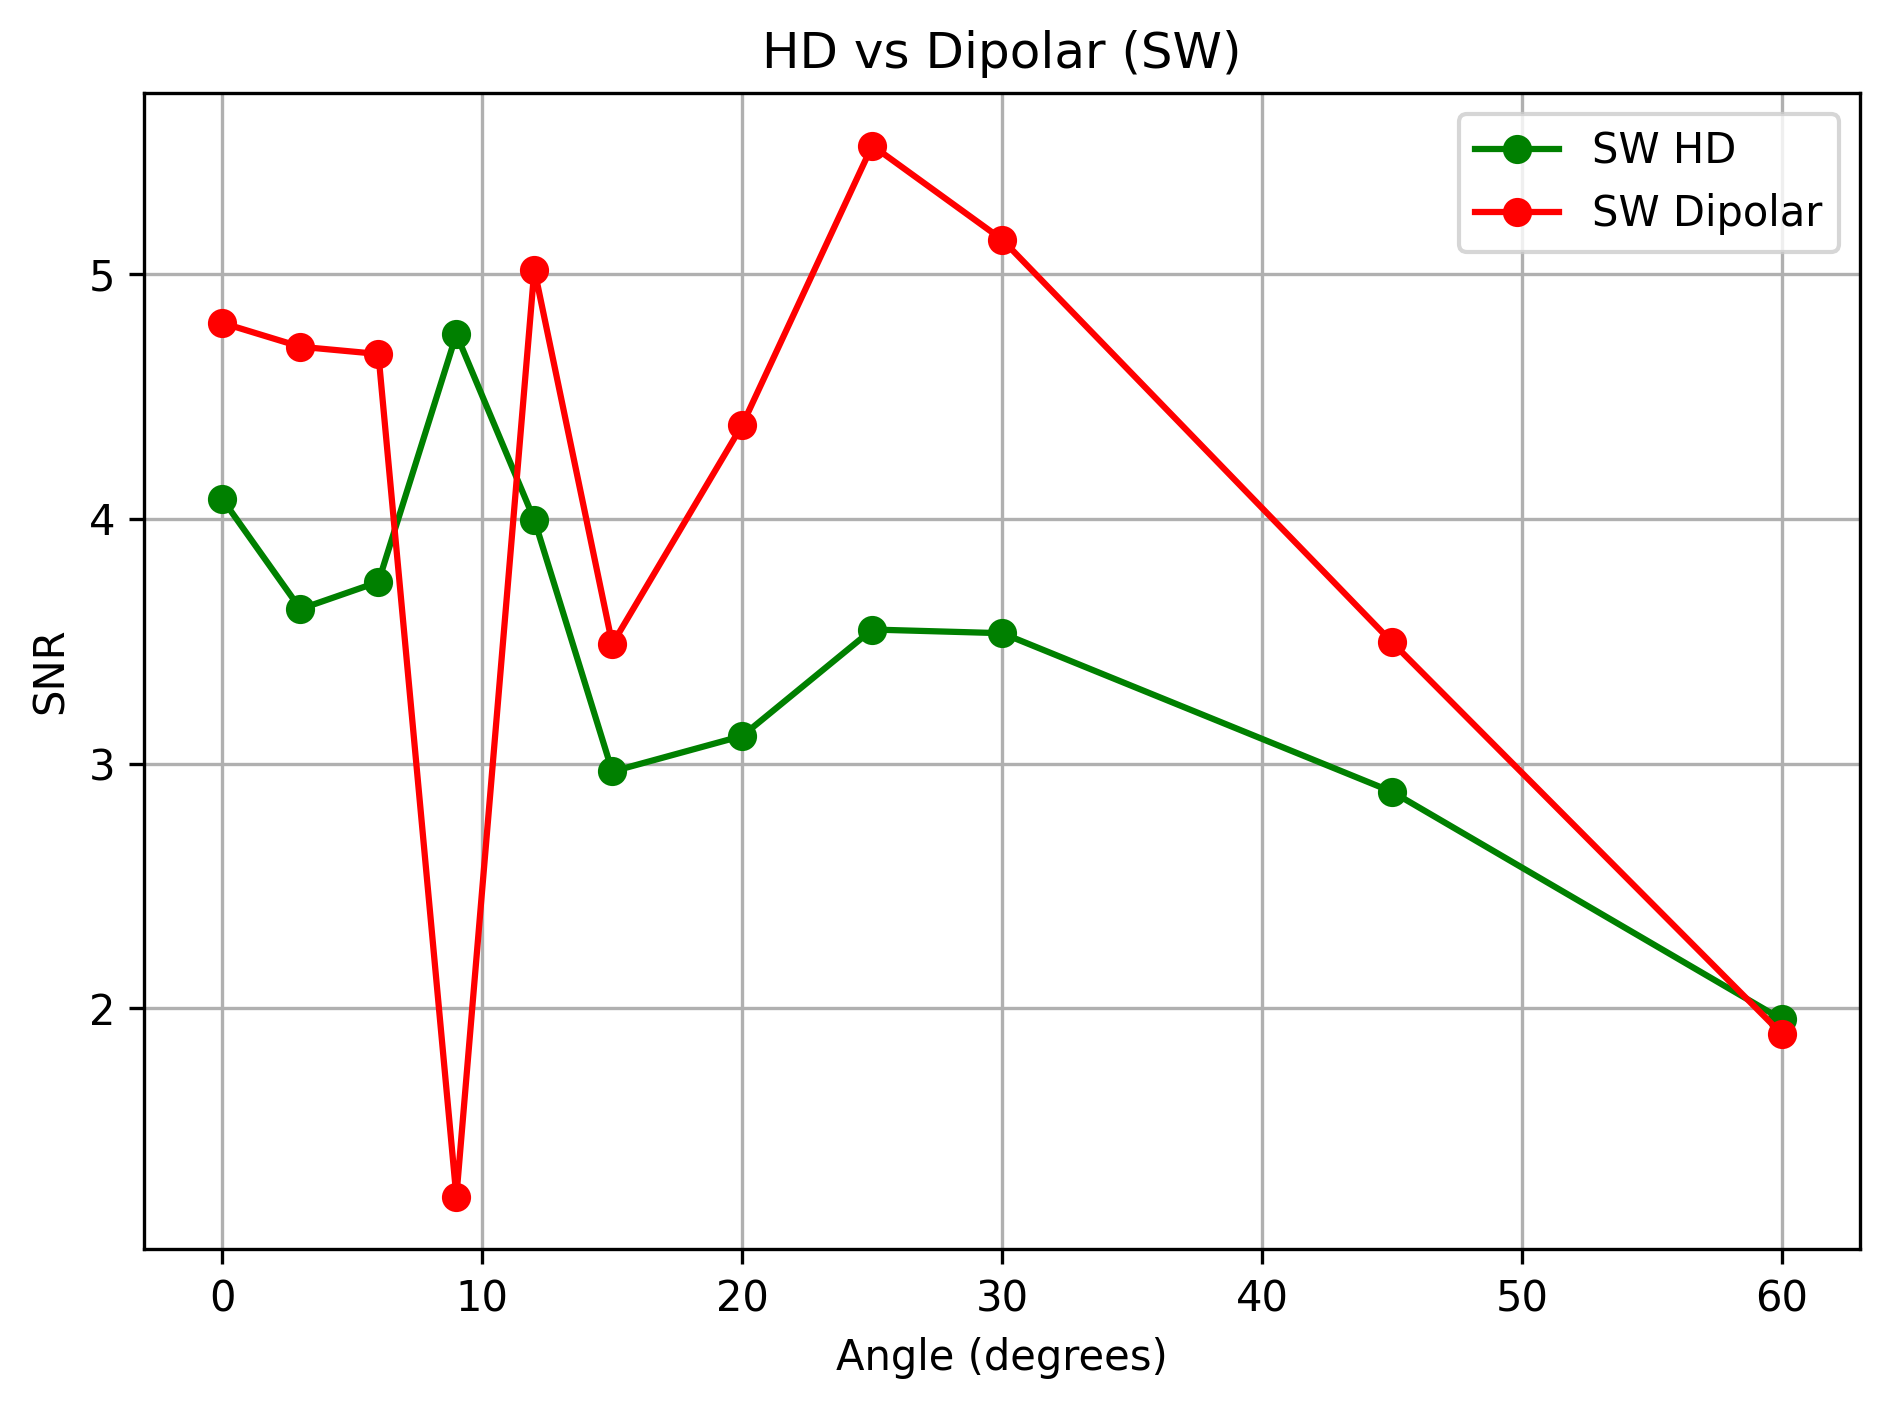
\includegraphics[width=\linewidth,height=0.38\textheight,keepaspectratio]{figures/image3.png}
    \caption{SNR\_HD and SNR\_dipolar with SW model}
    \label{fig:img3}
  \end{subfigure}
  \hfill
  \begin{subfigure}[b]{0.48\textwidth}
    \centering
    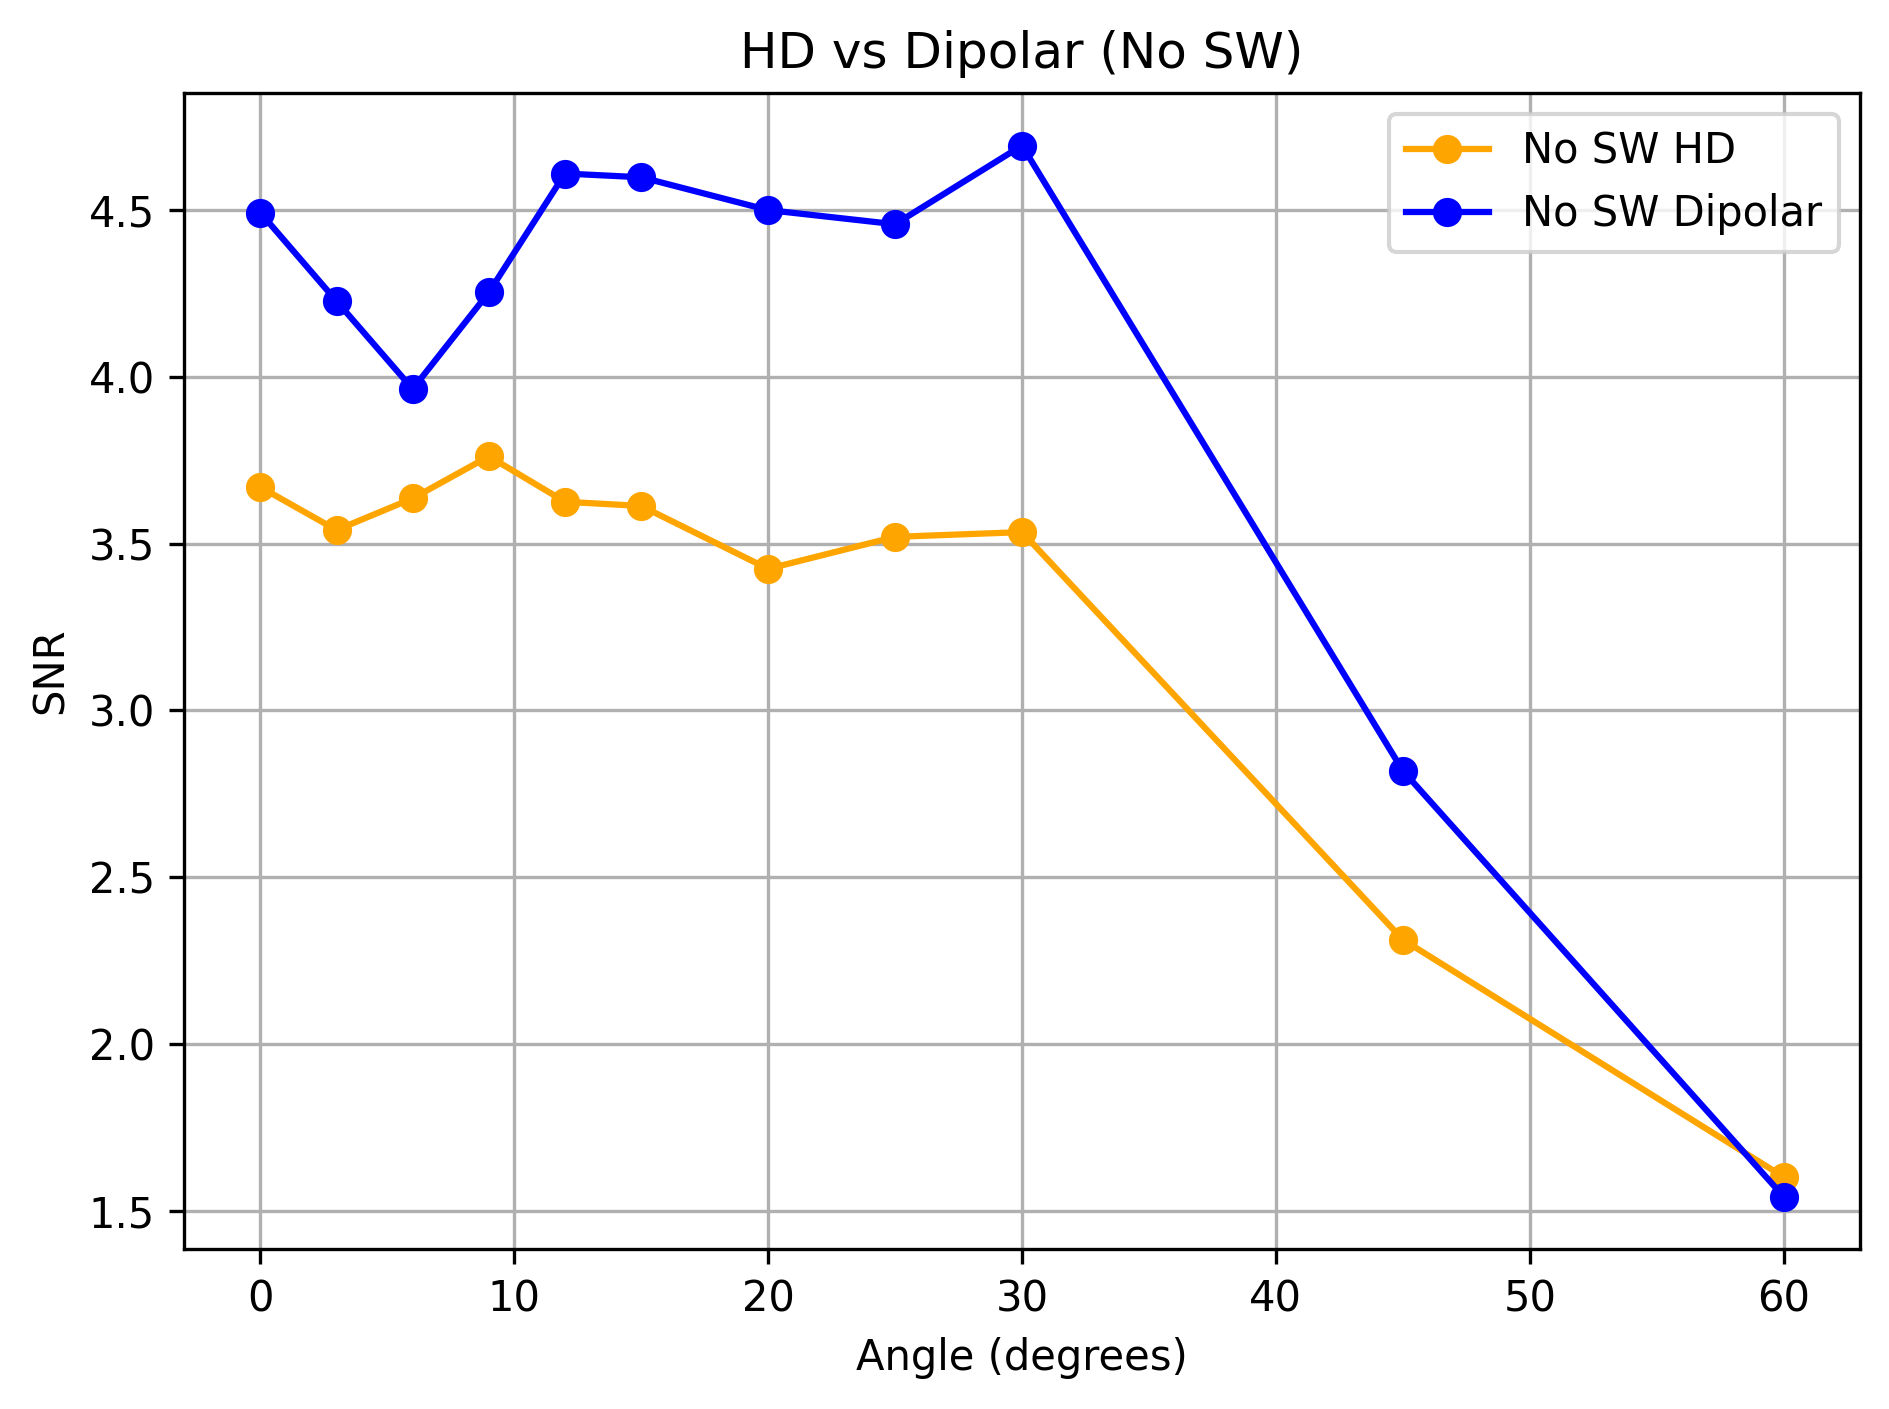
\includegraphics[width=\linewidth,height=0.38\textheight,keepaspectratio]{figures/image23.png}
    \caption{SNR\_HD and SNR\_dipolar with no\_SW model}
    \label{fig:img4}
  \end{subfigure}

  \caption{Global caption describing the 2×2 panel.}
  \label{fig:2x2_noborder}
\end{figure}




\section{Discussion and openings}
This work highlights several consistent themes: data selection strongly affects dipolar vs quadrupolar SNRs, FD removal can improve parameter constraints for some pulsars but may reduce TOA uncertainties artificially in others, and solar-proximity cuts have dataset-dependent impacts that interact with solar-wind modelling choices. ......

\section*{Acknowledgements}
I thank Hendrik and Saurav for providing templates and simulated datasets, and the MPTA team for guidance and feedback during the internship.

\section*{Appendix}


\end{document}